% Created 2019-08-25 dim. 21:03
% Intended LaTeX compiler: pdflatex
\documentclass[11pt]{article}
\usepackage[utf8]{inputenc}
\usepackage[T1]{fontenc}
\usepackage{graphicx}
\usepackage{grffile}
\usepackage{longtable}
\usepackage{wrapfig}
\usepackage{rotating}
\usepackage[normalem]{ulem}
\usepackage{amsmath}
\usepackage{textcomp}
\usepackage{amssymb}
\usepackage{capt-of}
\usepackage{hyperref}
\usepackage{minitoc}
\date{}
\title{TMP Chem Notebook}
\hypersetup{
 pdfauthor={haina},
 pdftitle={TMP Chem Notebook},
 pdfkeywords={},
 pdfsubject={},
 pdfcreator={Emacs 26.1 (Org mode 9.2.5)}, 
 pdflang={English}}
\begin{document}

\maketitle
\dosecttoc
\pagebreak[4] \setcounter{tocdepth}{1} \tableofcontents \pagebreak[4] \setcounter{tocdepth}{2} 
\section{Math }
\label{sec:org114c2aa}
\secttoc \pagebreak[4]
\subsection{Introduction}
\label{sec:orga7359f0}
\makebox[\textwidth][c]{
\begin{center}
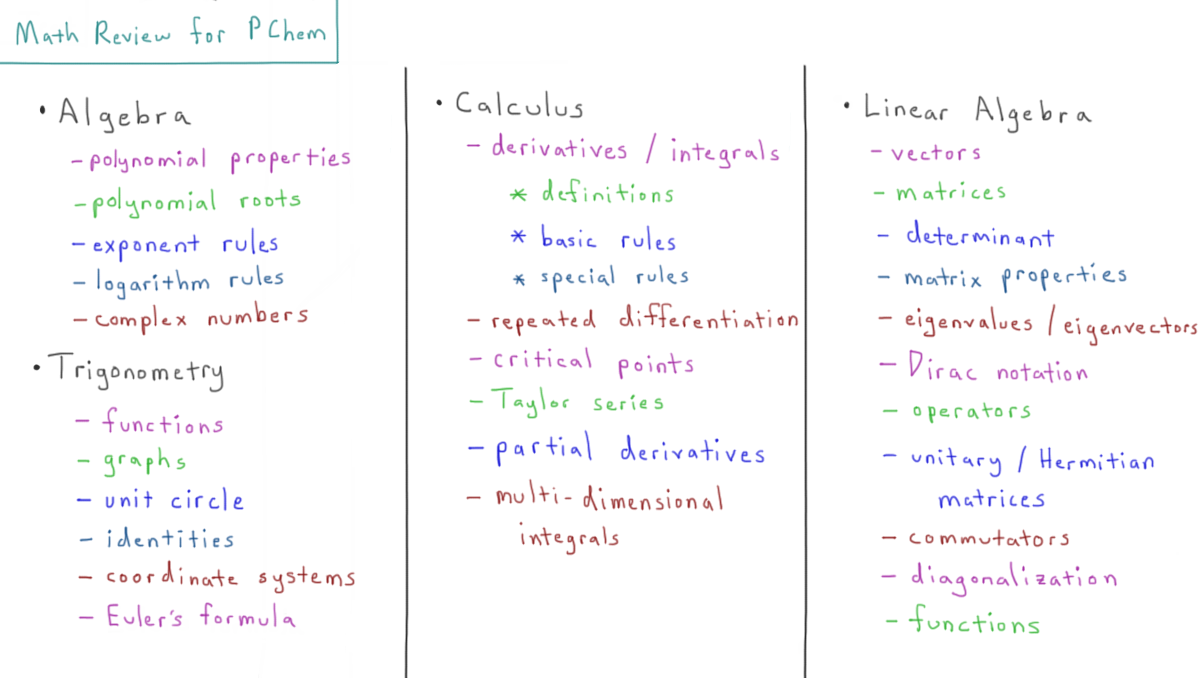
\includegraphics[width=1.2\textwidth]{./tmp_proc_img/Math/0.png}
\end{center}
}

\pagebreak[4]
\subsection{Polynomial Properties}
\label{sec:orgfce932a}
\makebox[\textwidth][c]{
\begin{center}
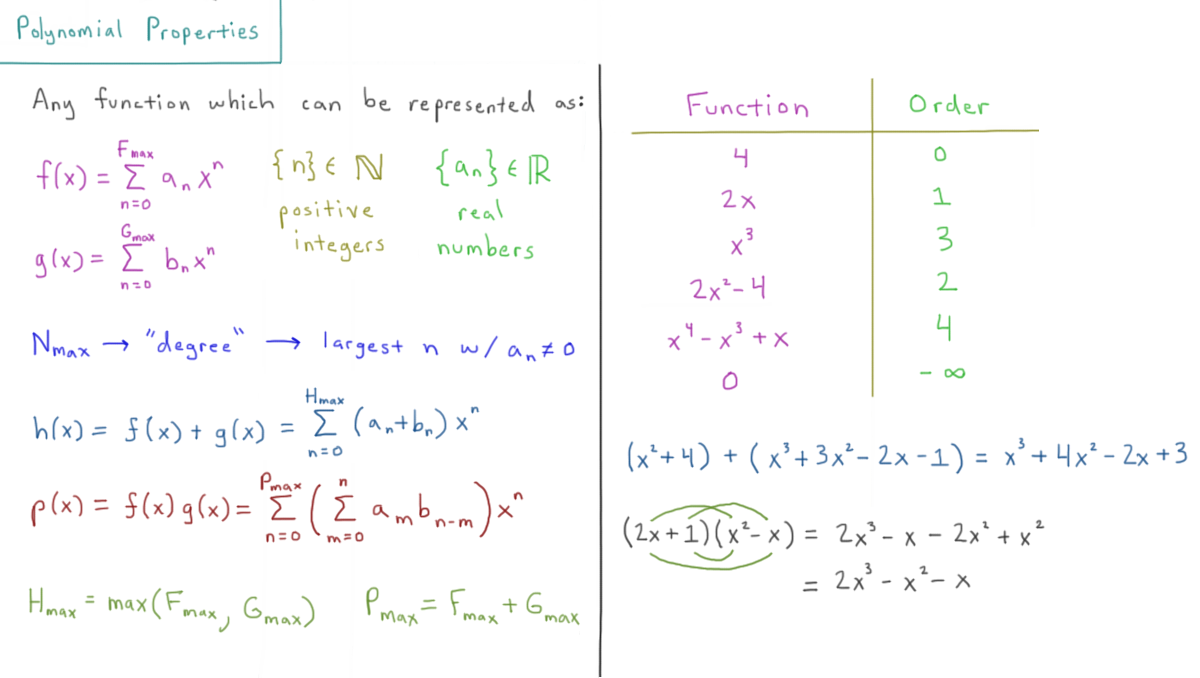
\includegraphics[width=1.2\textwidth]{./tmp_proc_img/Math/1.png}
\end{center}
}

\pagebreak[4]
\subsection{Polynomial Roots}
\label{sec:org7fbdebb}
\makebox[\textwidth][c]{
\begin{center}
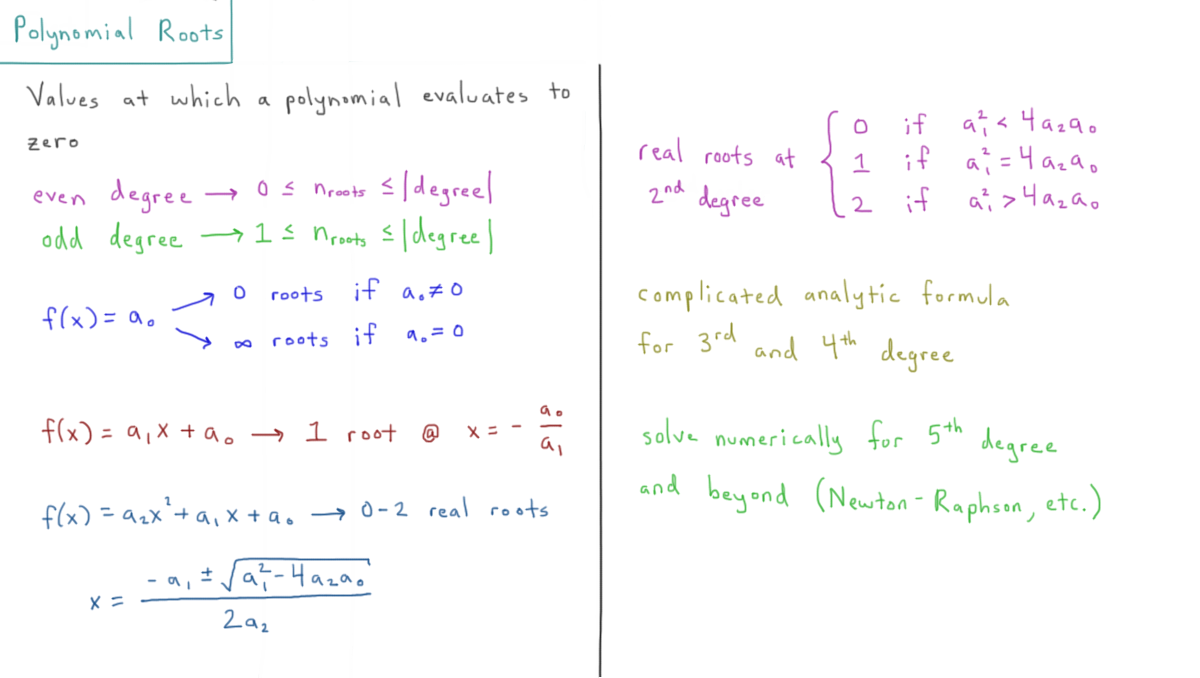
\includegraphics[width=1.2\textwidth]{./tmp_proc_img/Math/2.png}
\end{center}
}

\pagebreak[4]
\subsection{Exponent and Logarithm Properties}
\label{sec:orgfd3b059}
\makebox[\textwidth][c]{
\begin{center}
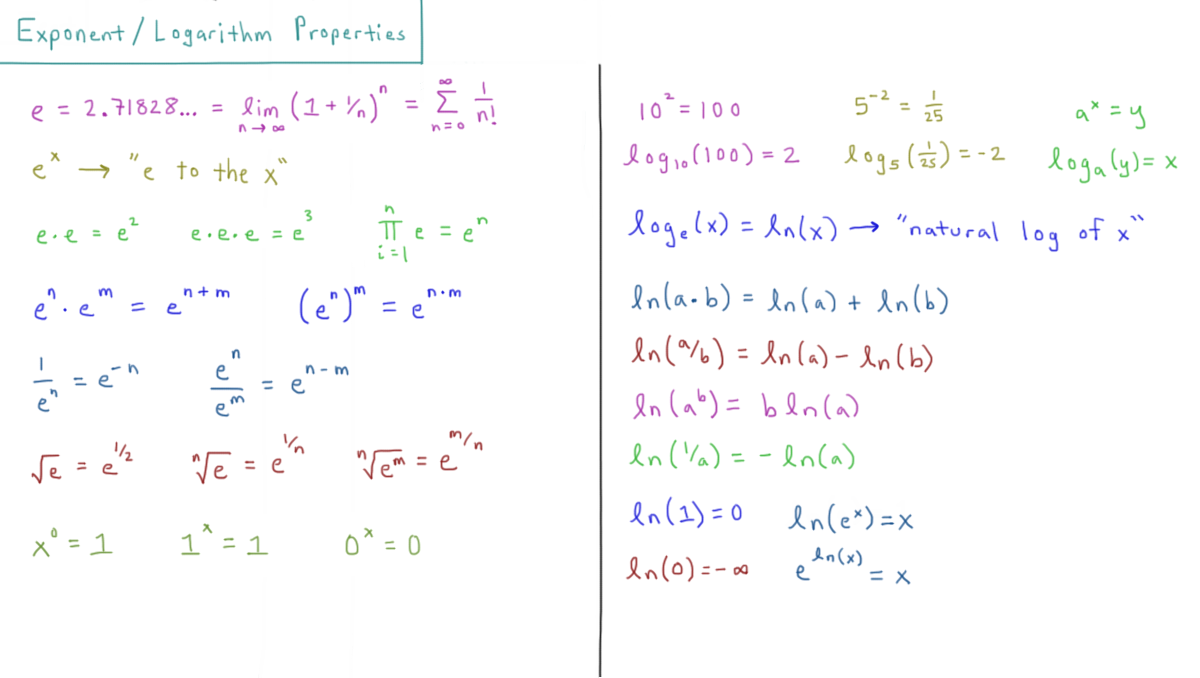
\includegraphics[width=1.2\textwidth]{./tmp_proc_img/Math/3.png}
\end{center}
}

\pagebreak[4]
\subsection{Complex Numbers}
\label{sec:orge31325e}
\makebox[\textwidth][c]{
\begin{center}
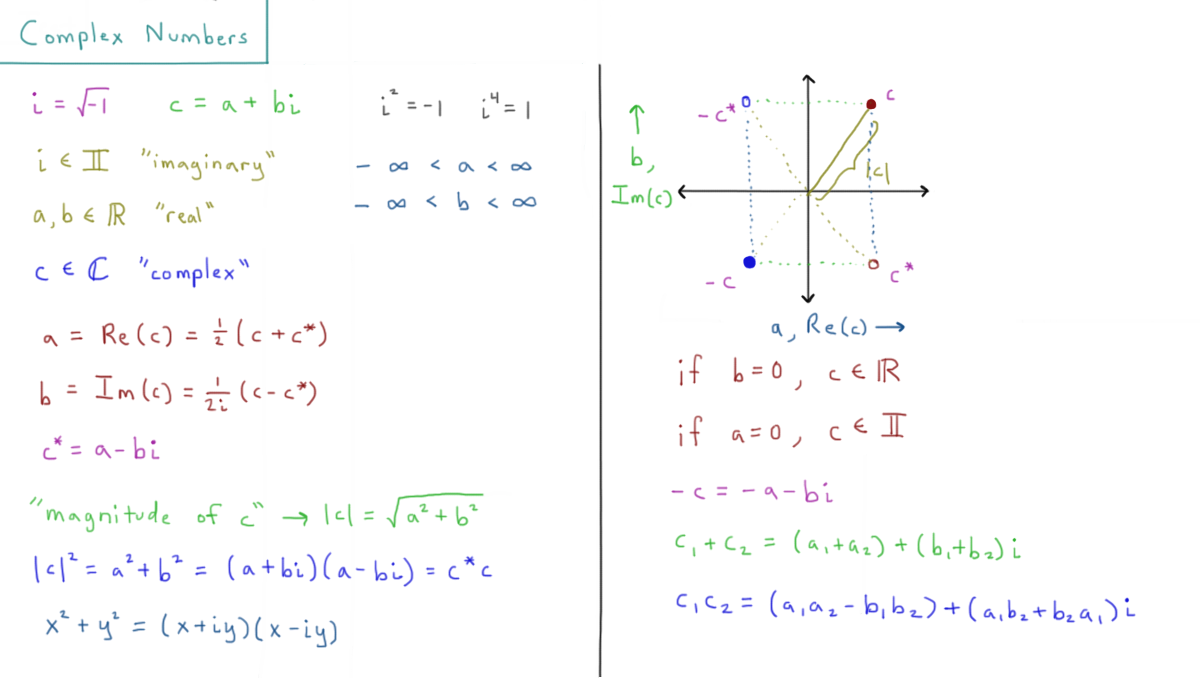
\includegraphics[width=1.2\textwidth]{./tmp_proc_img/Math/4.png}
\end{center}
}

\pagebreak[4]
\subsection{Trigonometric Functions}
\label{sec:org65e2dea}
\makebox[\textwidth][c]{
\begin{center}
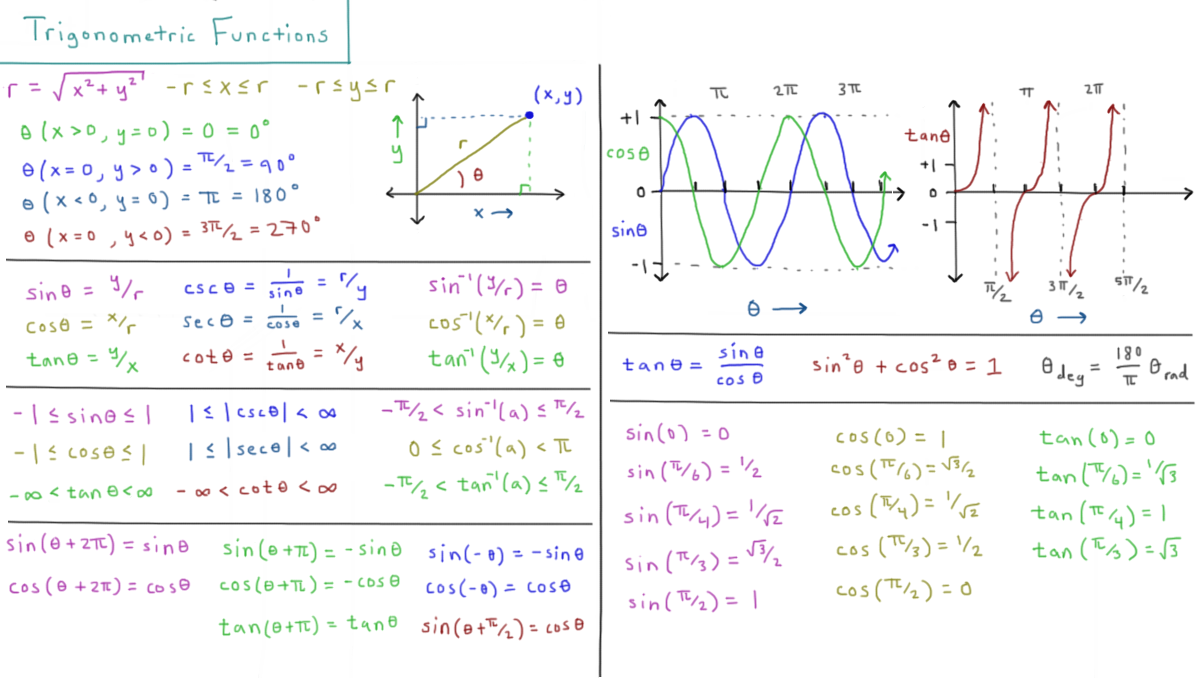
\includegraphics[width=1.2\textwidth]{./tmp_proc_img/Math/5.png}
\end{center}
}

\pagebreak[4]
\subsection{Spherical and Polar Coordinates}
\label{sec:org06646a9}
\makebox[\textwidth][c]{
\begin{center}
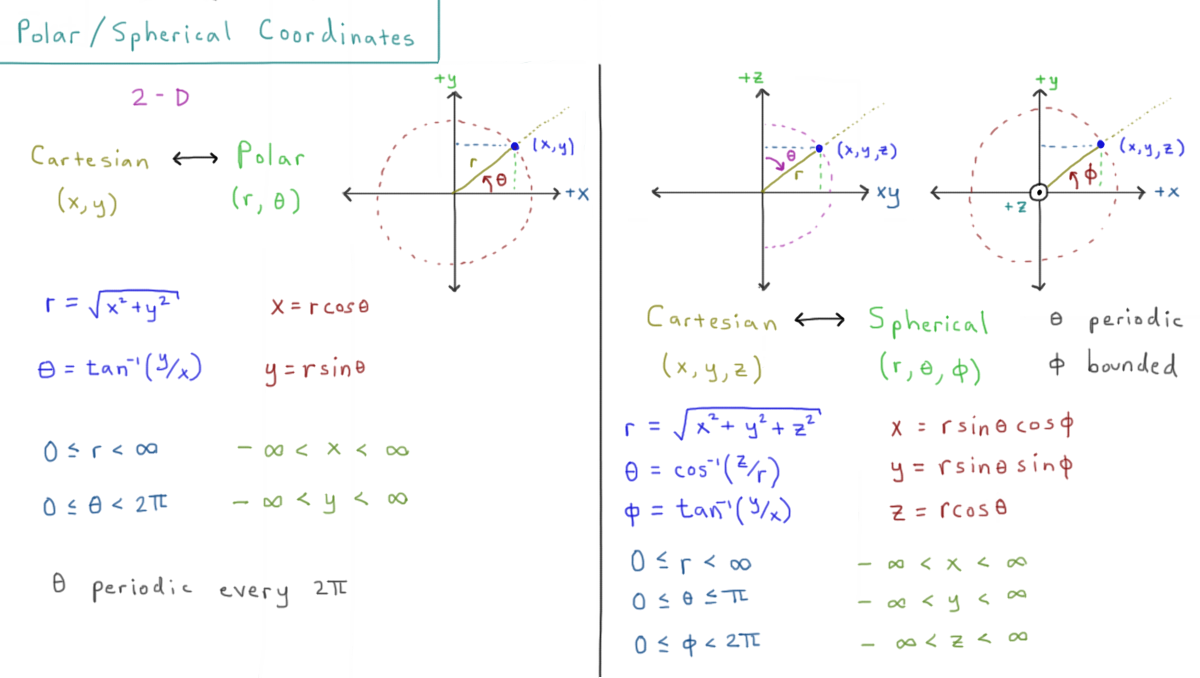
\includegraphics[width=1.2\textwidth]{./tmp_proc_img/Math/6.png}
\end{center}
}

\pagebreak[4]
\subsection{Derivative Definition}
\label{sec:orgd7f698d}
\makebox[\textwidth][c]{
\begin{center}
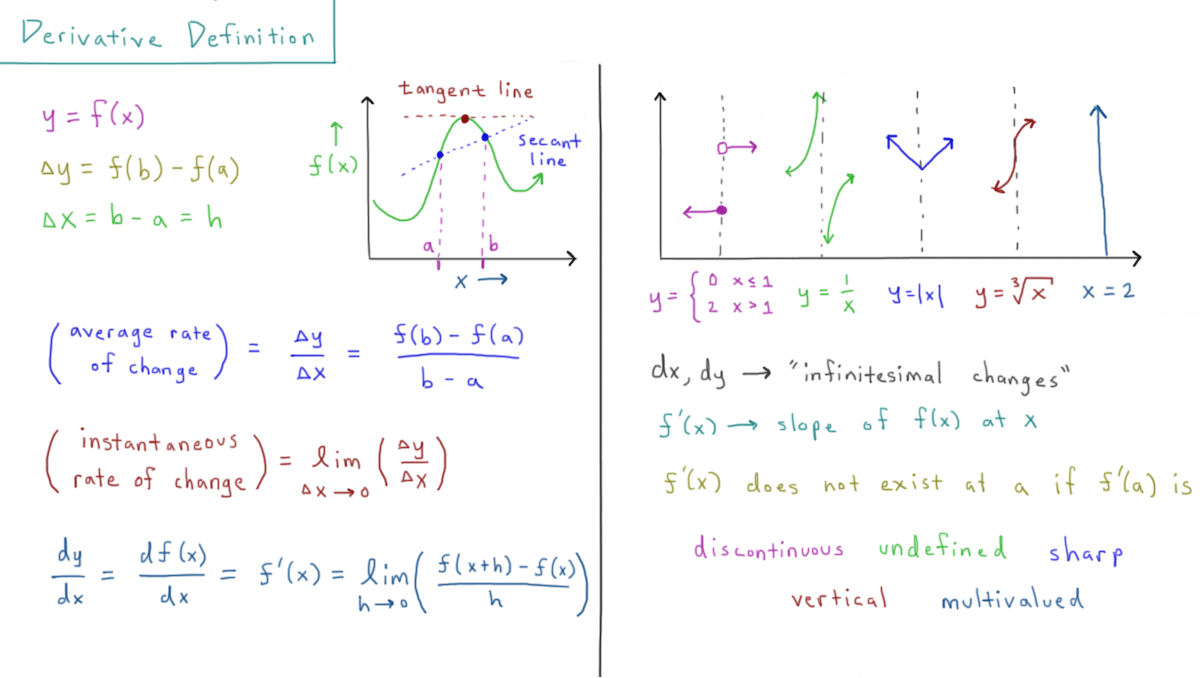
\includegraphics[width=1.2\textwidth]{./tmp_proc_img/Math/7.png}
\end{center}
}

\pagebreak[4]
\subsection{Basic Derivatives}
\label{sec:org1072783}
\makebox[\textwidth][c]{
\begin{center}
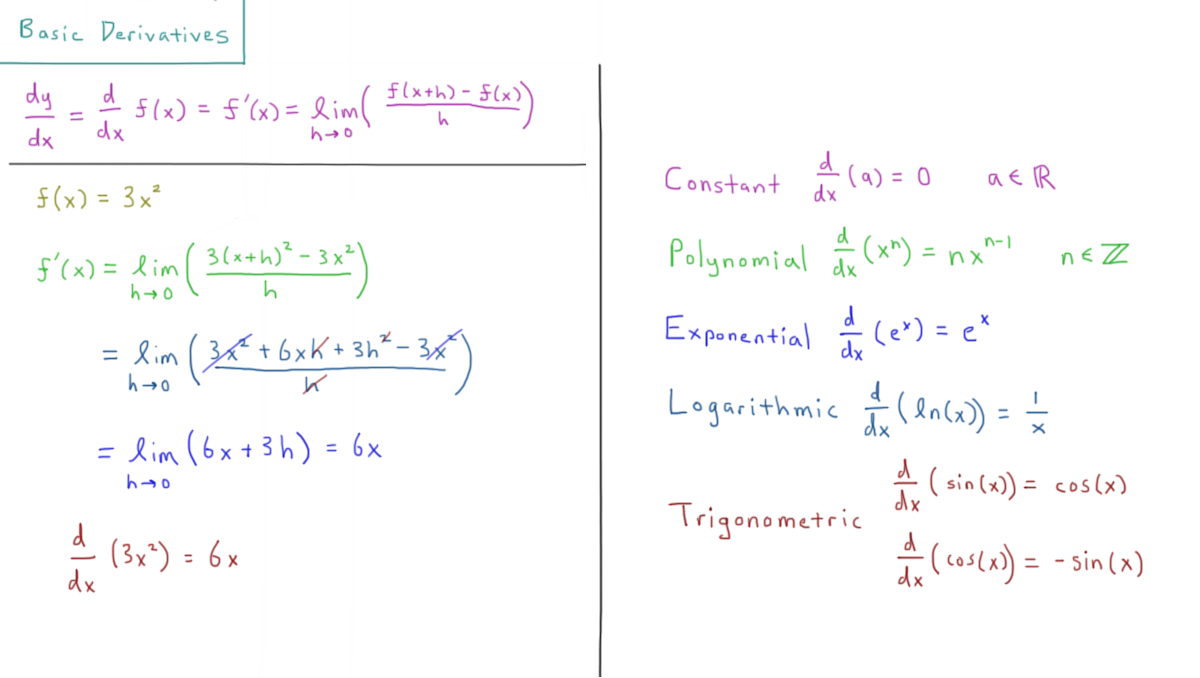
\includegraphics[width=1.2\textwidth]{./tmp_proc_img/Math/8.png}
\end{center}
}

\pagebreak[4]
\subsection{Derivative Rules}
\label{sec:orga446330}
\makebox[\textwidth][c]{
\begin{center}
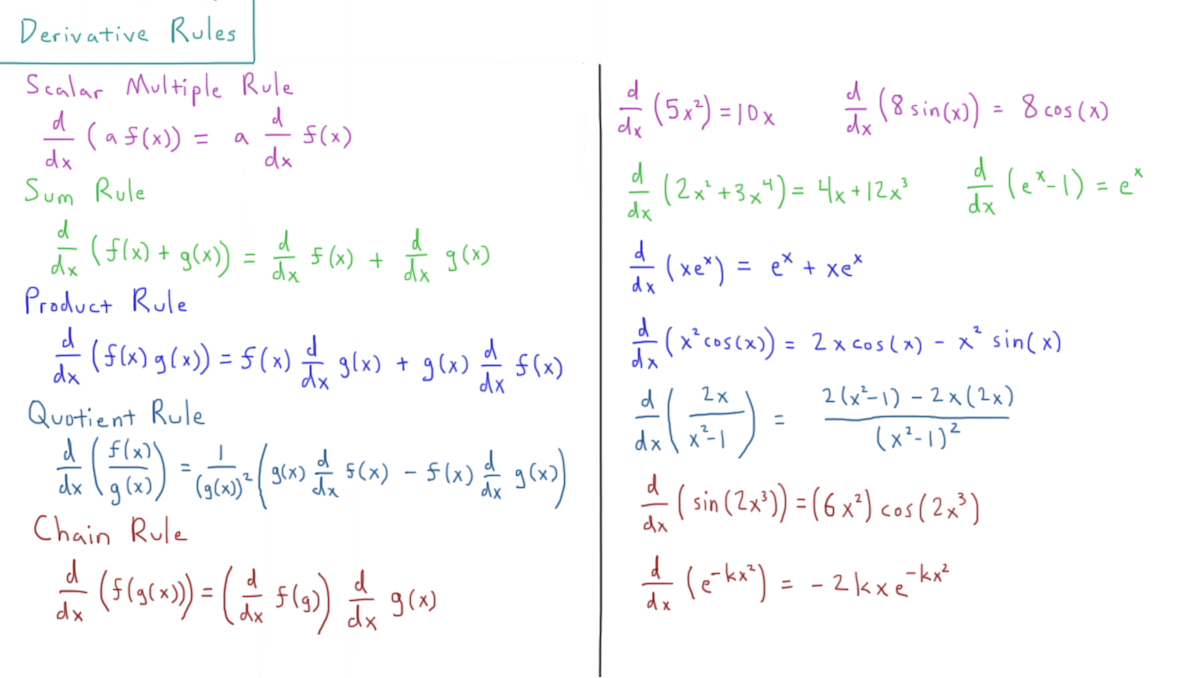
\includegraphics[width=1.2\textwidth]{./tmp_proc_img/Math/9.png}
\end{center}
}

\pagebreak[4]
\subsection{Repeated Derivatives}
\label{sec:org4a7f880}
\makebox[\textwidth][c]{
\begin{center}
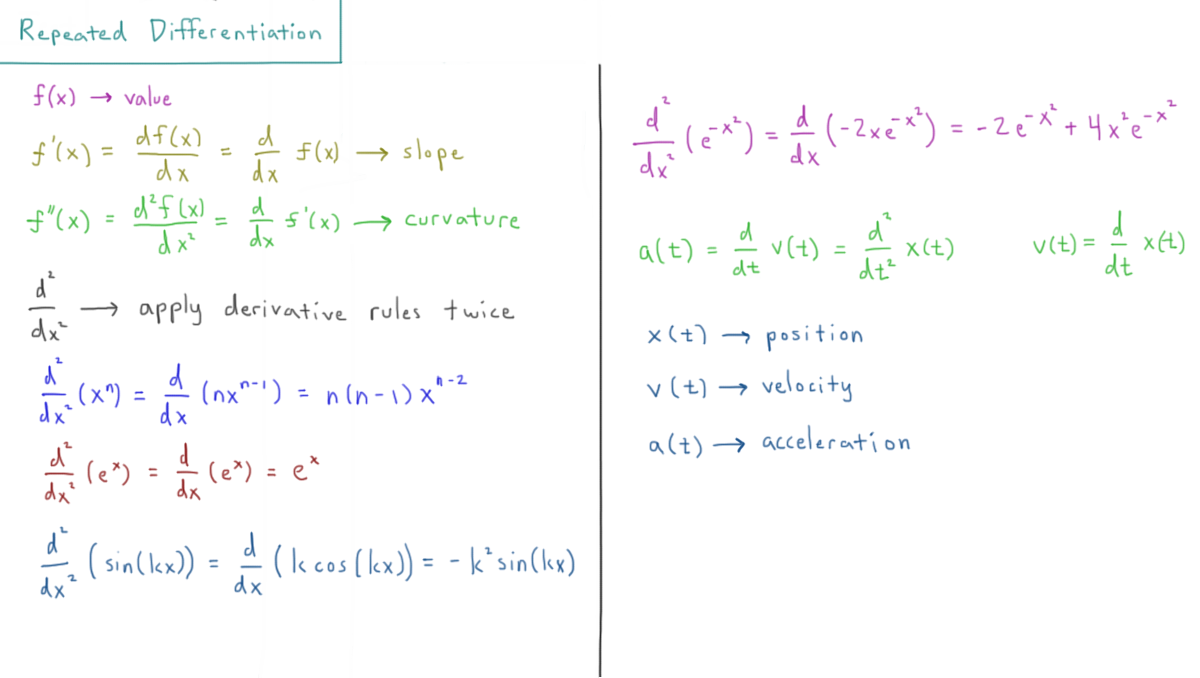
\includegraphics[width=1.2\textwidth]{./tmp_proc_img/Math/10.png}
\end{center}
}

\pagebreak[4]
\subsection{Function Critical Points}
\label{sec:orgbc3fb8e}
\makebox[\textwidth][c]{
\begin{center}
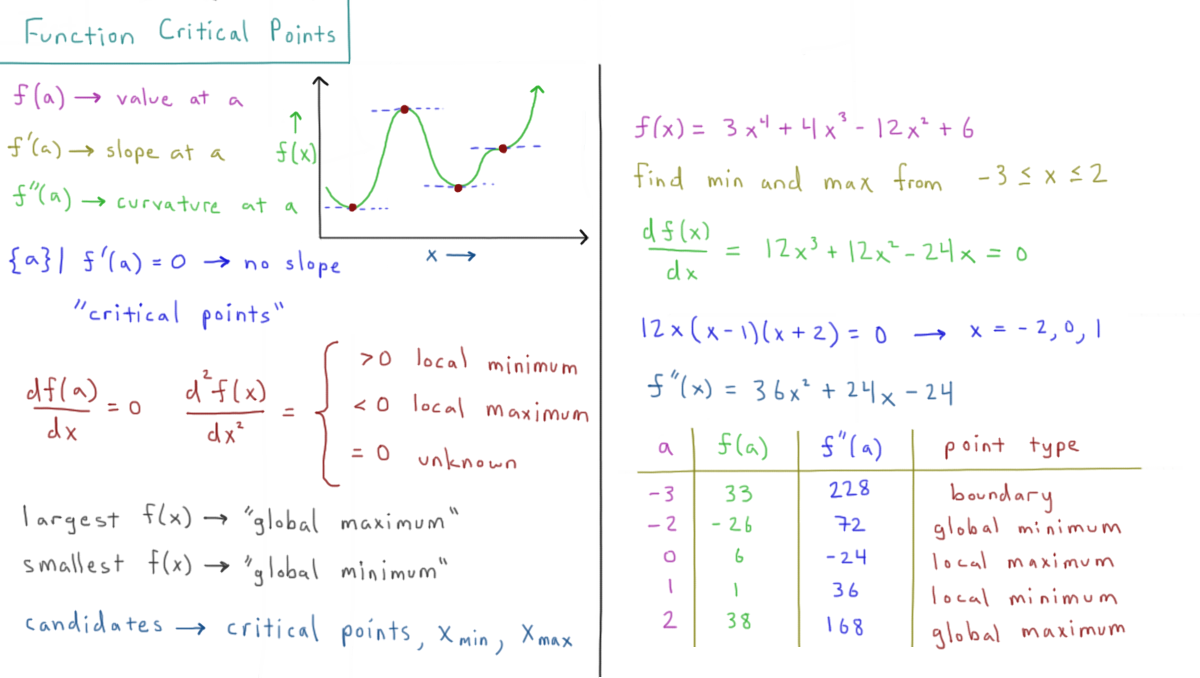
\includegraphics[width=1.2\textwidth]{./tmp_proc_img/Math/11.png}
\end{center}
}

\pagebreak[4]
\subsection{Taylor Series}
\label{sec:org327cf73}
\makebox[\textwidth][c]{
\begin{center}
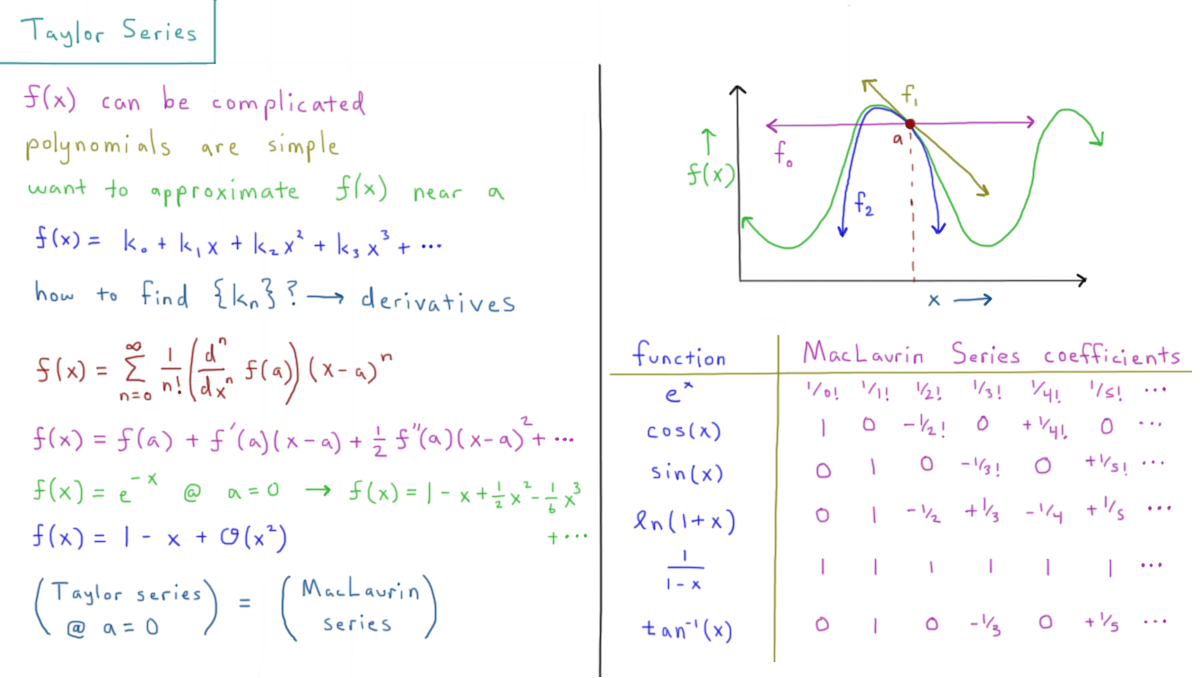
\includegraphics[width=1.2\textwidth]{./tmp_proc_img/Math/12.png}
\end{center}
}

\pagebreak[4]
\subsection{Integral Definition}
\label{sec:orgf15f525}
\makebox[\textwidth][c]{
\begin{center}
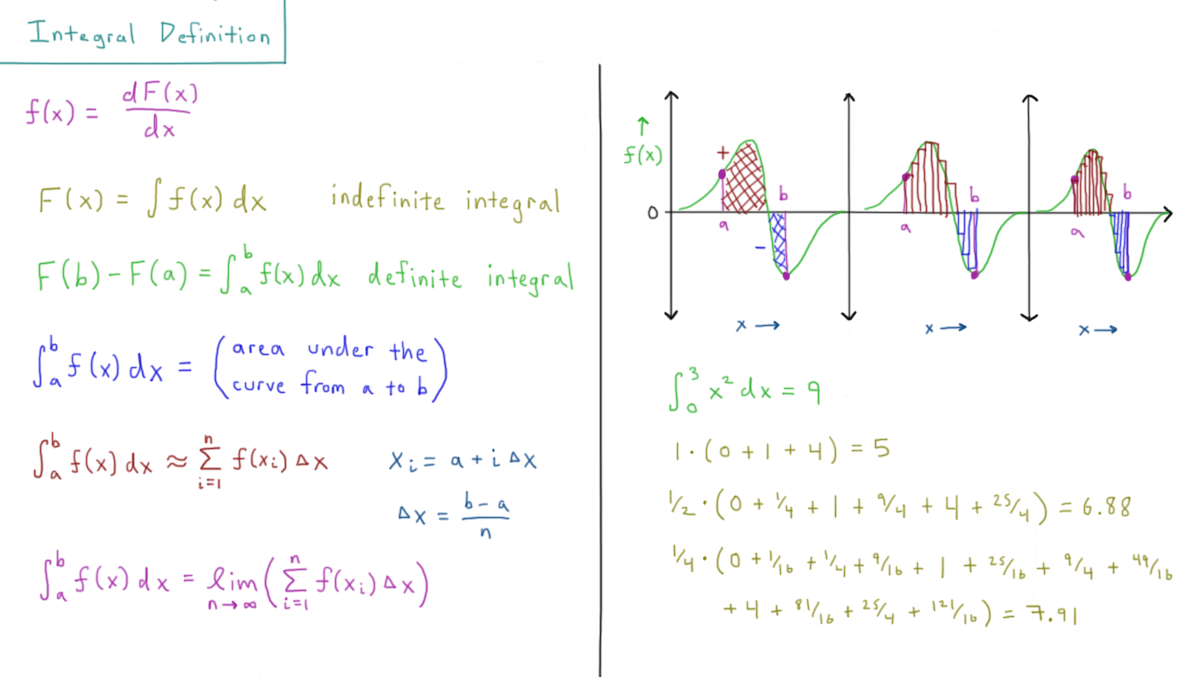
\includegraphics[width=1.2\textwidth]{./tmp_proc_img/Math/13.png}
\end{center}
}

\pagebreak[4]
\subsection{Basic Integrals}
\label{sec:org00d312b}
\makebox[\textwidth][c]{
\begin{center}
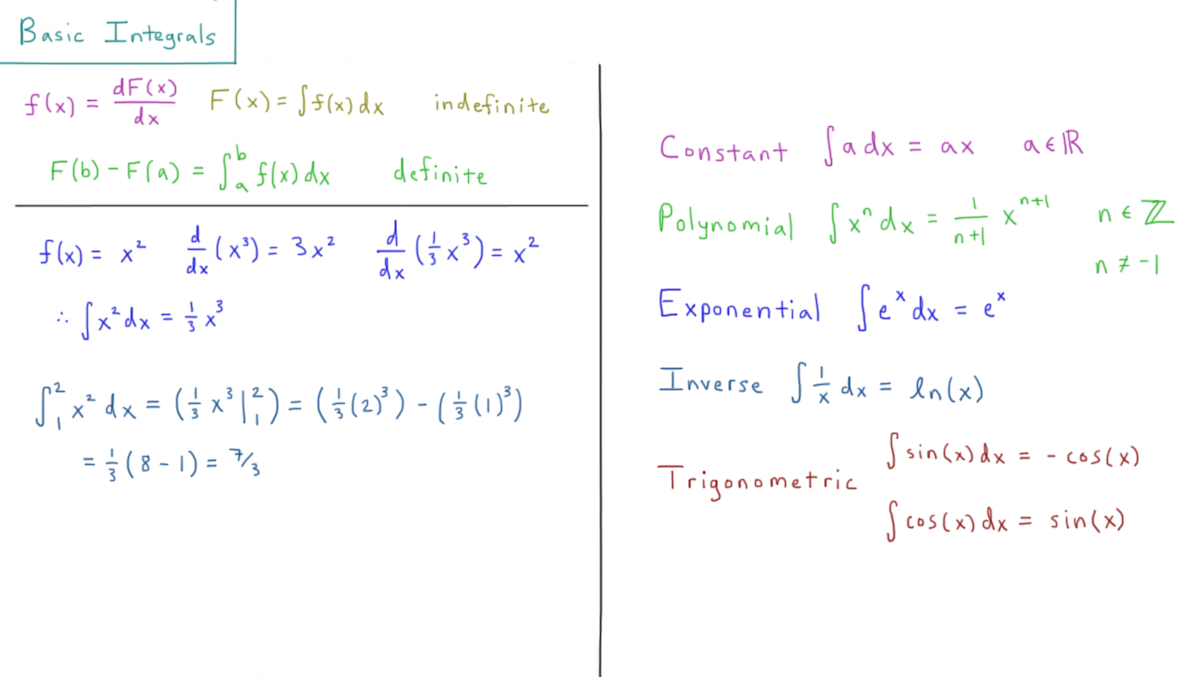
\includegraphics[width=1.2\textwidth]{./tmp_proc_img/Math/14.png}
\end{center}
}

\pagebreak[4]
\subsection{Integral Rules}
\label{sec:org50030b3}
\makebox[\textwidth][c]{
\begin{center}
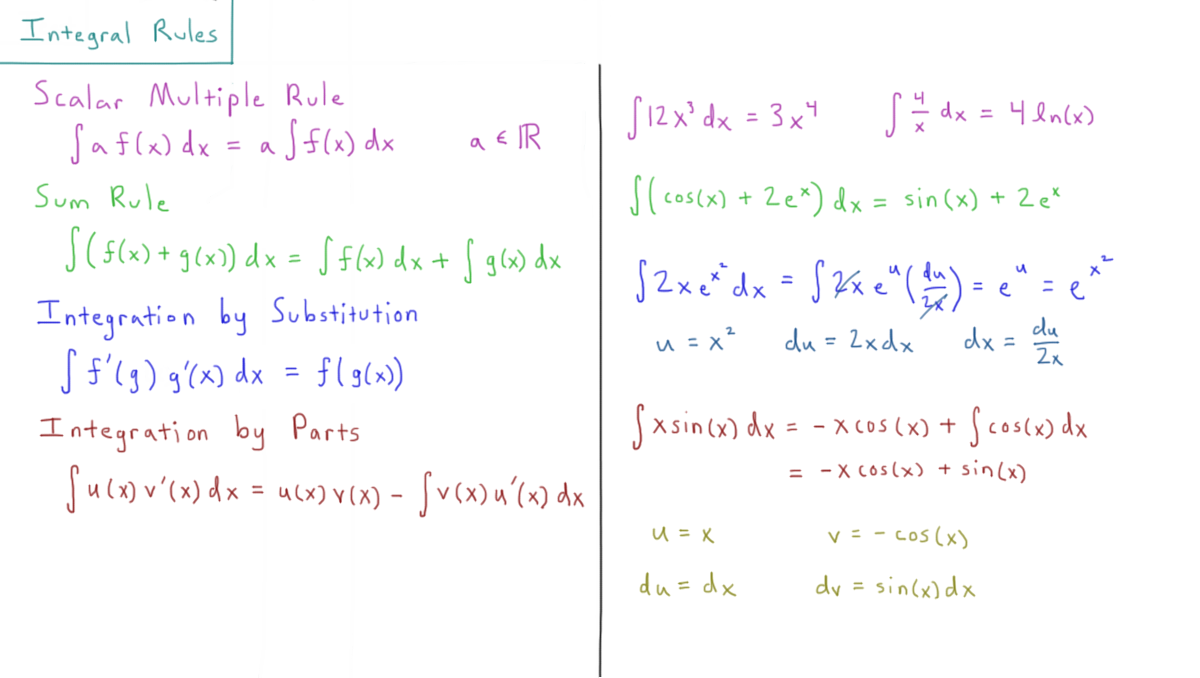
\includegraphics[width=1.2\textwidth]{./tmp_proc_img/Math/15.png}
\end{center}
}

\pagebreak[4]
\subsection{Partial Derivatives}
\label{sec:org0d2ccdb}
\makebox[\textwidth][c]{
\begin{center}
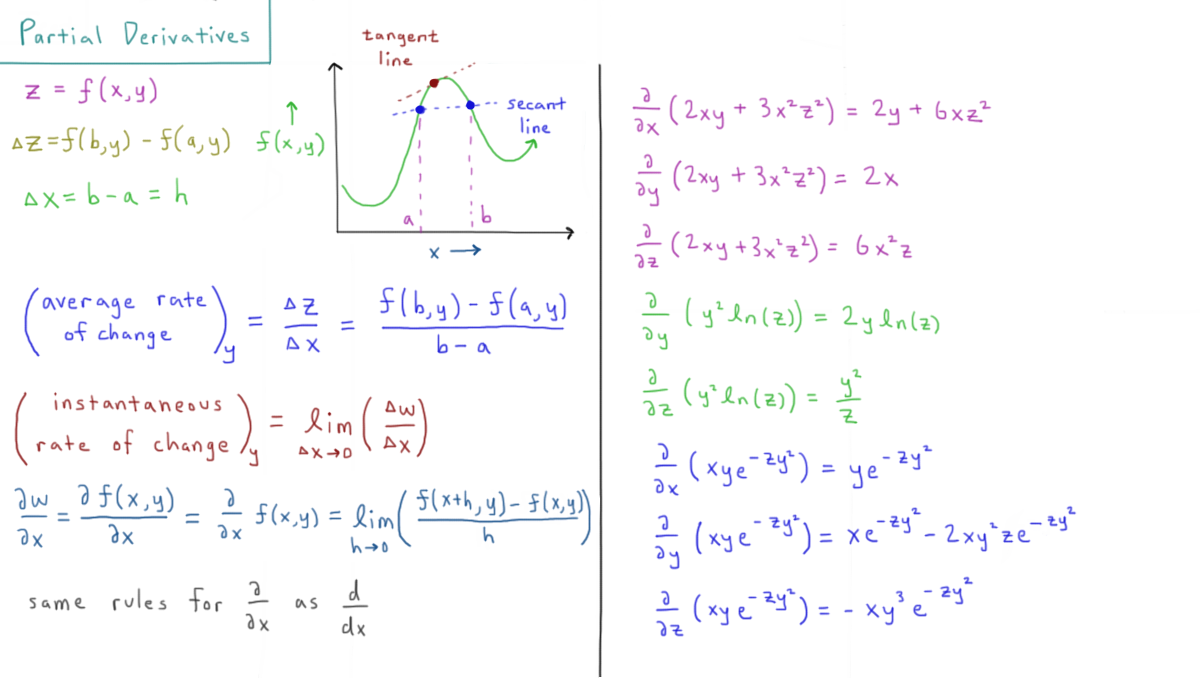
\includegraphics[width=1.2\textwidth]{./tmp_proc_img/Math/16.png}
\end{center}
}

\pagebreak[4]
\subsection{Repeated Partial Derivatives}
\label{sec:orga7f3446}
\makebox[\textwidth][c]{
\begin{center}
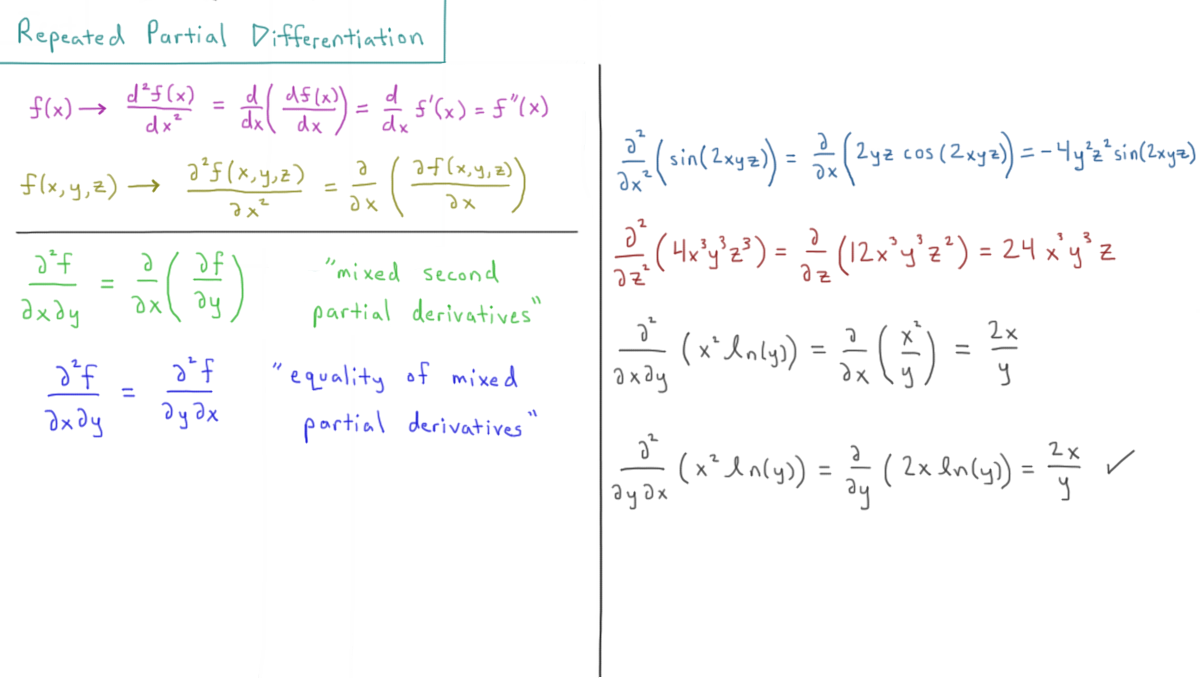
\includegraphics[width=1.2\textwidth]{./tmp_proc_img/Math/17.png}
\end{center}
}

\pagebreak[4]
\subsection{Multi-Dimensional Integrals}
\label{sec:org1f62a08}
\makebox[\textwidth][c]{
\begin{center}
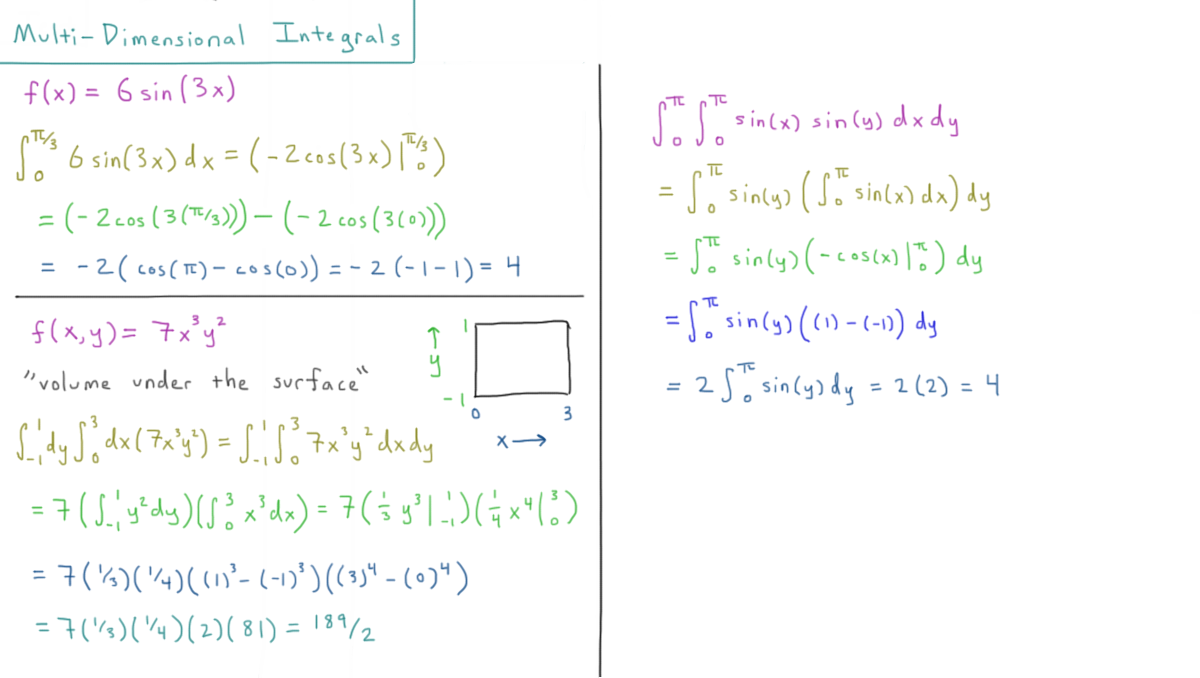
\includegraphics[width=1.2\textwidth]{./tmp_proc_img/Math/18.png}
\end{center}
}

\pagebreak[4]
\subsection{Volume Elements}
\label{sec:org19b6bcc}
\makebox[\textwidth][c]{
\begin{center}
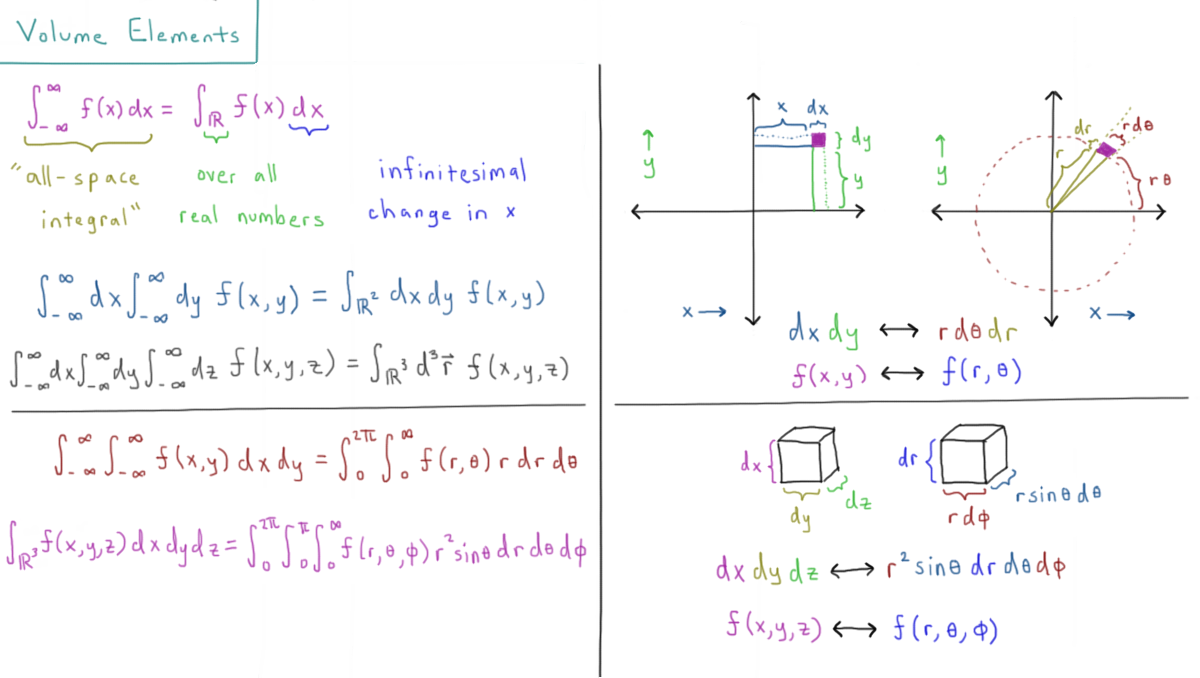
\includegraphics[width=1.2\textwidth]{./tmp_proc_img/Math/19.png}
\end{center}
}

\pagebreak[4]
\subsection{Euler's Formula}
\label{sec:org880221b}
\makebox[\textwidth][c]{
\begin{center}
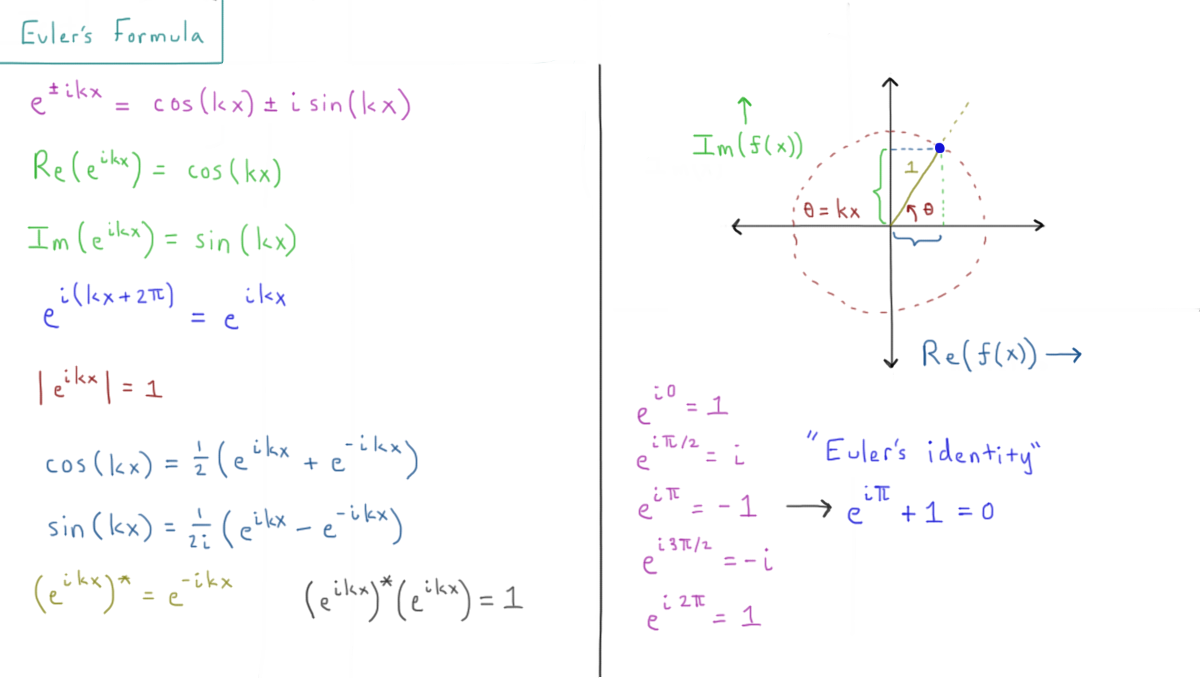
\includegraphics[width=1.2\textwidth]{./tmp_proc_img/Math/20.png}
\end{center}
}

\pagebreak[4]
\subsection{Vectors}
\label{sec:org3a45c7b}
\makebox[\textwidth][c]{
\begin{center}
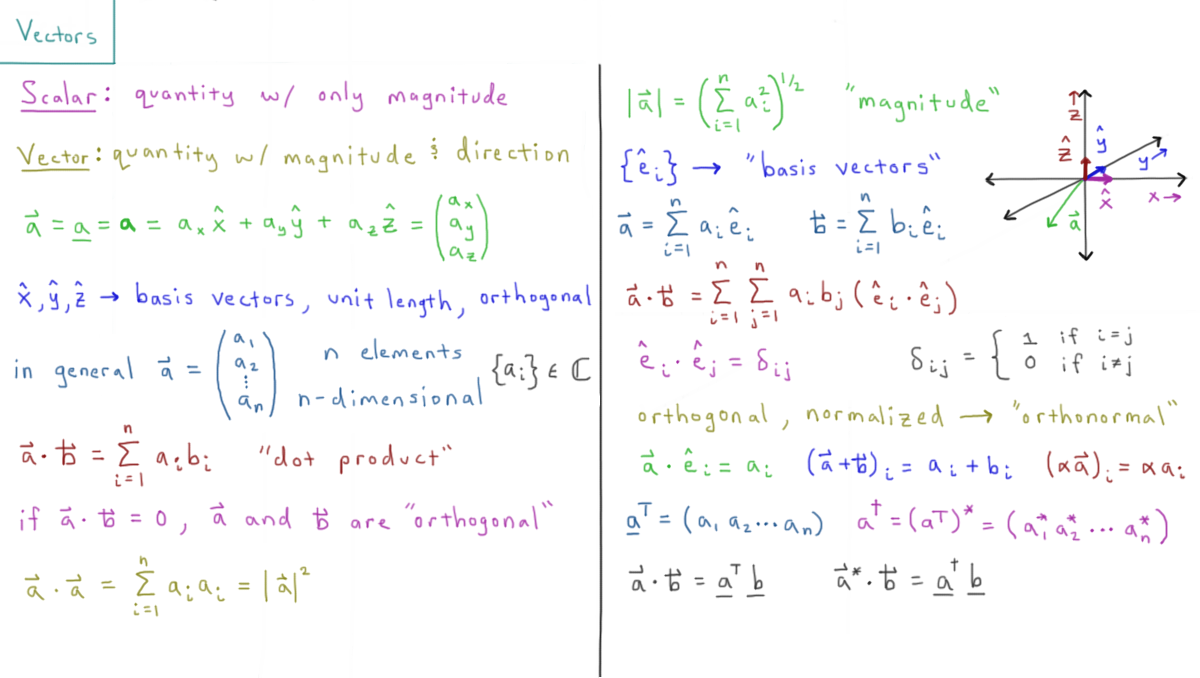
\includegraphics[width=1.2\textwidth]{./tmp_proc_img/Math/21.png}
\end{center}
}

\pagebreak[4]
\subsection{Matrices}
\label{sec:org08caa9f}
\makebox[\textwidth][c]{
\begin{center}
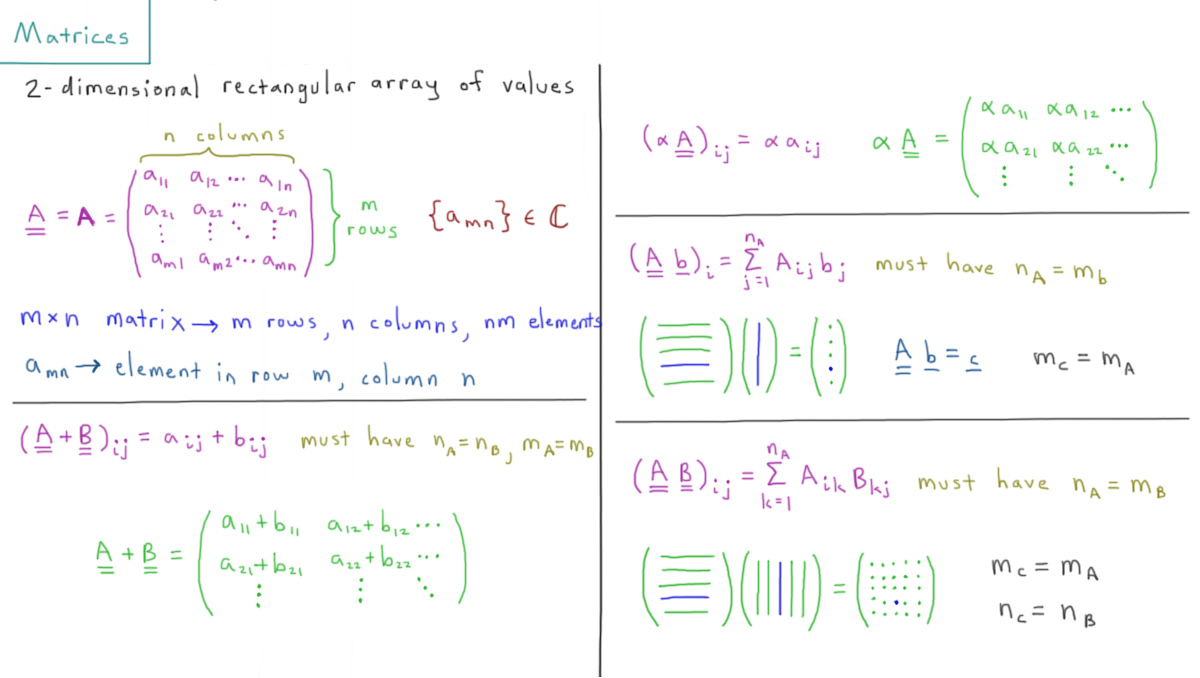
\includegraphics[width=1.2\textwidth]{./tmp_proc_img/Math/22.png}
\end{center}
}

\pagebreak[4]
\subsection{Determinants}
\label{sec:orgaa96675}
\makebox[\textwidth][c]{
\begin{center}
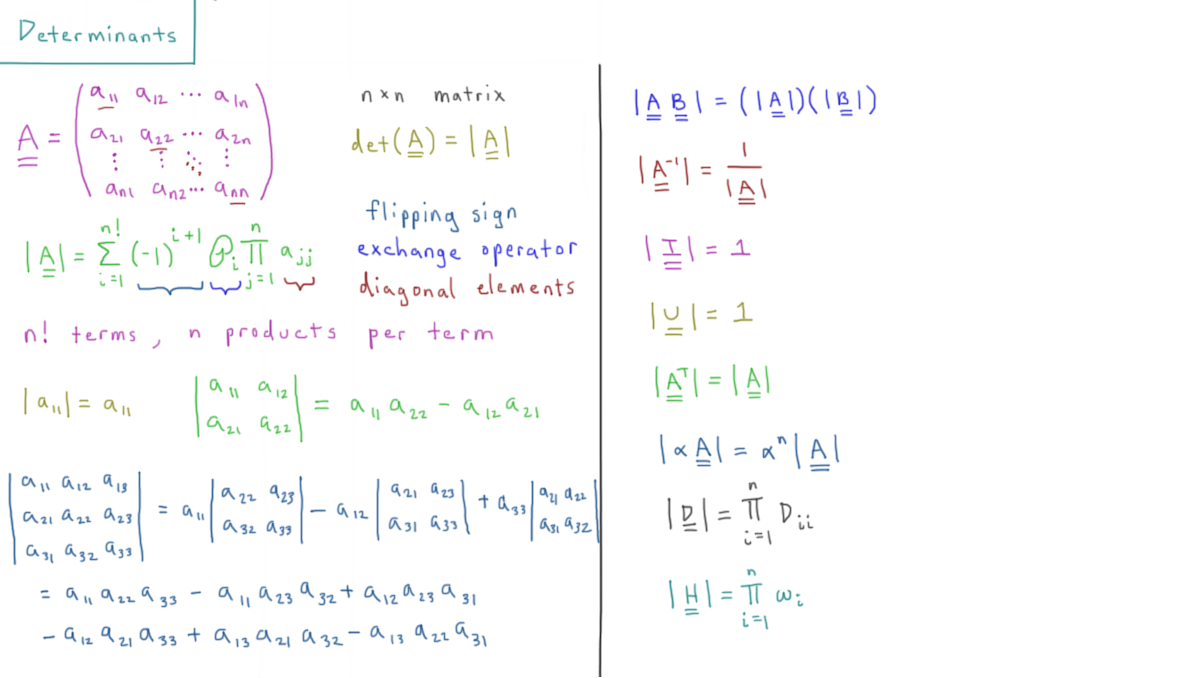
\includegraphics[width=1.2\textwidth]{./tmp_proc_img/Math/23.png}
\end{center}
}

\pagebreak[4]
\subsection{Matrix Properties}
\label{sec:orgcae2d8a}
\makebox[\textwidth][c]{
\begin{center}
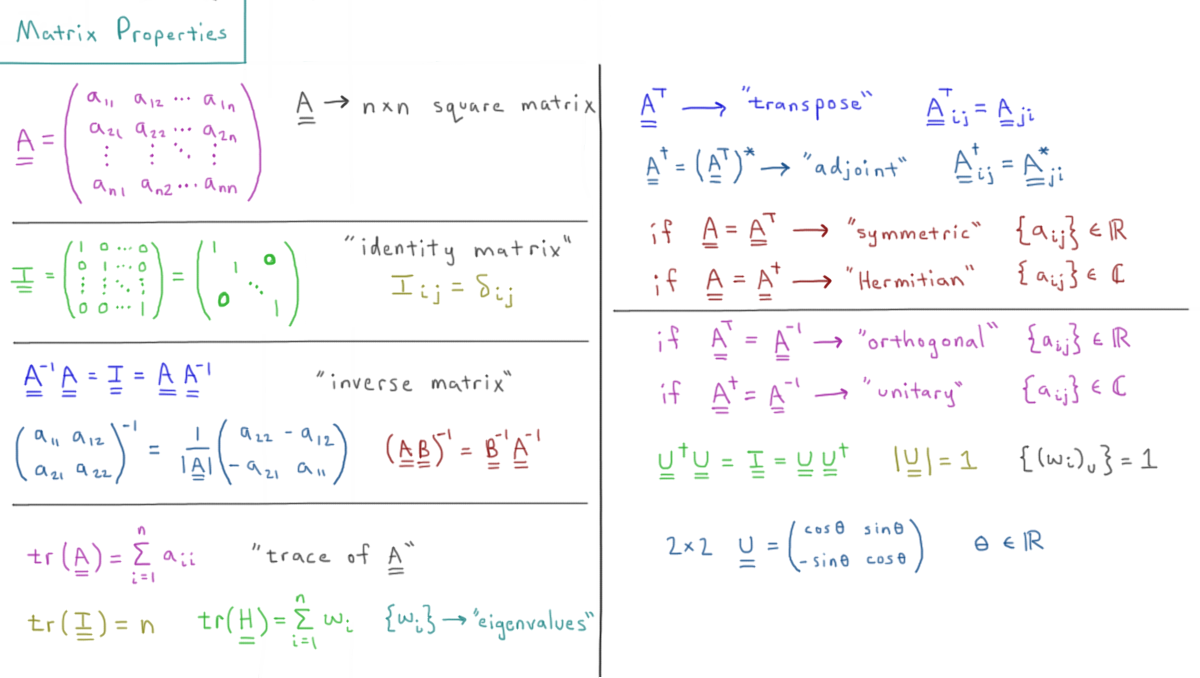
\includegraphics[width=1.2\textwidth]{./tmp_proc_img/Math/24.png}
\end{center}
}

\pagebreak[4]
\subsection{Matrix Eigenvalues and Eigenvectors}
\label{sec:org817e475}
\makebox[\textwidth][c]{
\begin{center}
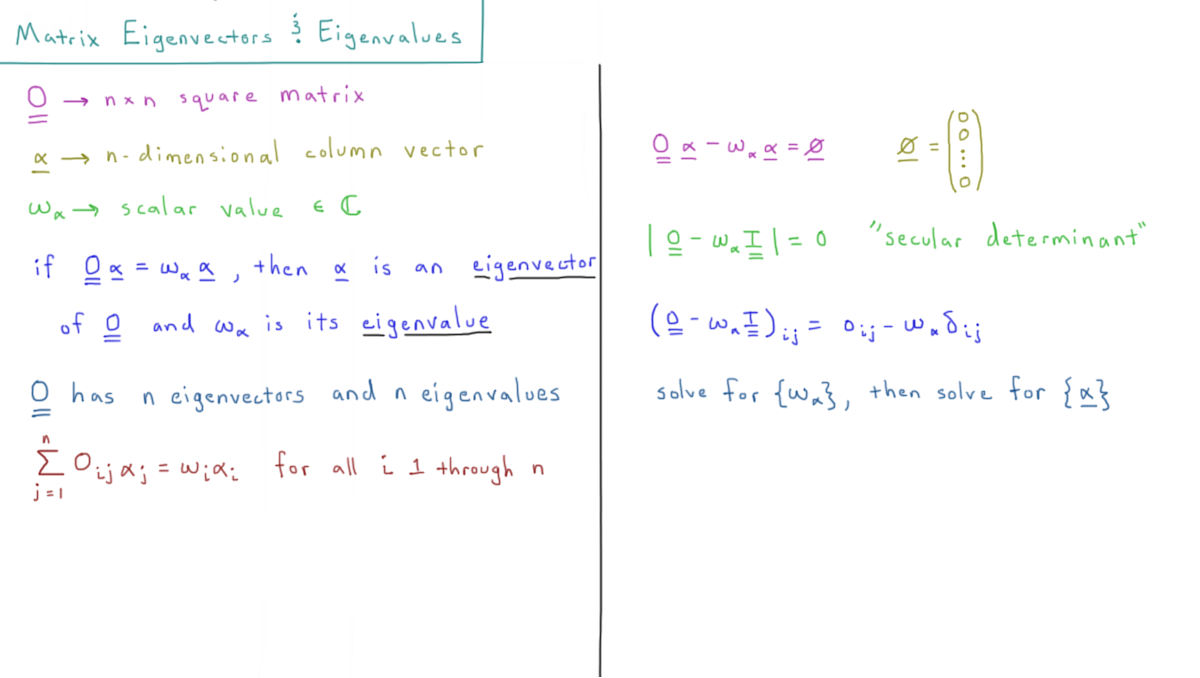
\includegraphics[width=1.2\textwidth]{./tmp_proc_img/Math/25.png}
\end{center}
}

\pagebreak[4]
\subsection{Discrete Dirac Notation}
\label{sec:orgd1163a7}
\makebox[\textwidth][c]{
\begin{center}
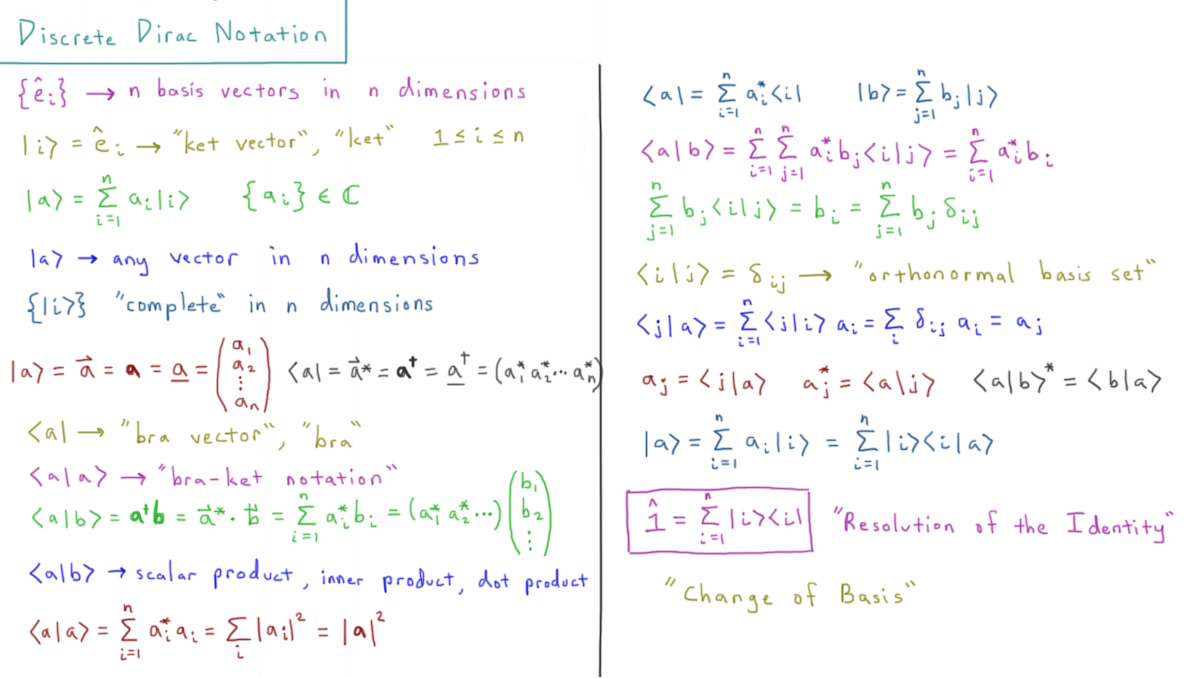
\includegraphics[width=1.2\textwidth]{./tmp_proc_img/Math/26.png}
\end{center}
}

\pagebreak[4]
\subsection{Matrix Operators}
\label{sec:org7068b0b}
\makebox[\textwidth][c]{
\begin{center}
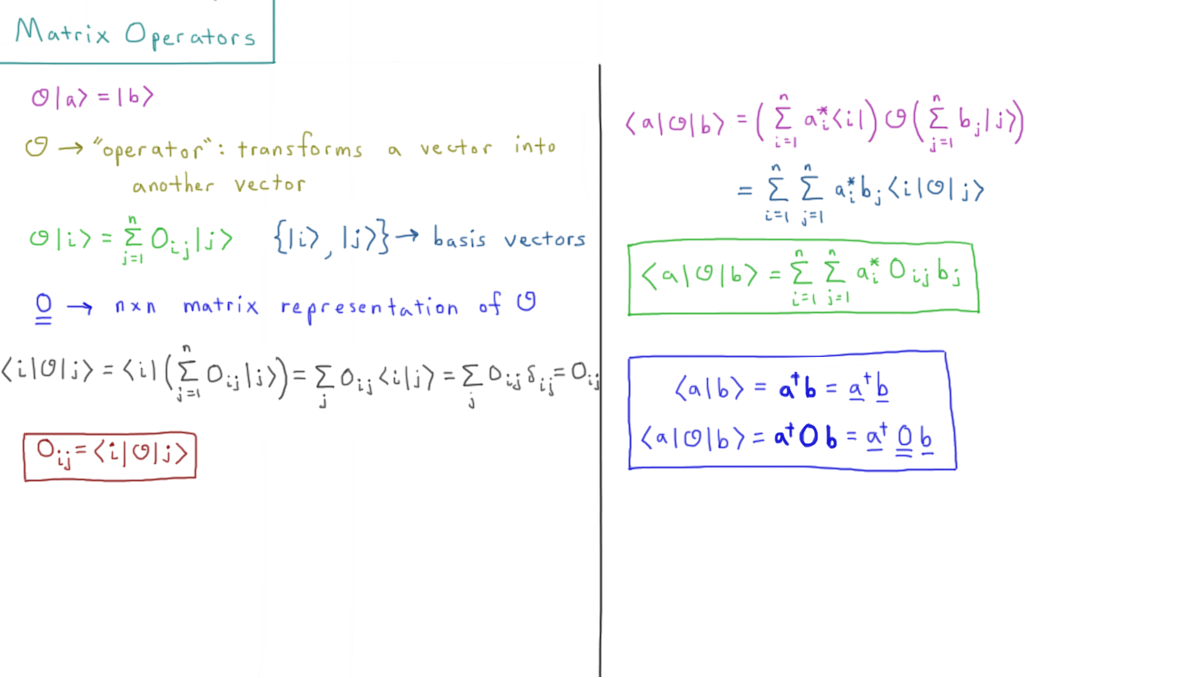
\includegraphics[width=1.2\textwidth]{./tmp_proc_img/Math/27.png}
\end{center}
}

\pagebreak[4]
\subsection{Unitary Transformation}
\label{sec:org293fb8f}
\makebox[\textwidth][c]{
\begin{center}
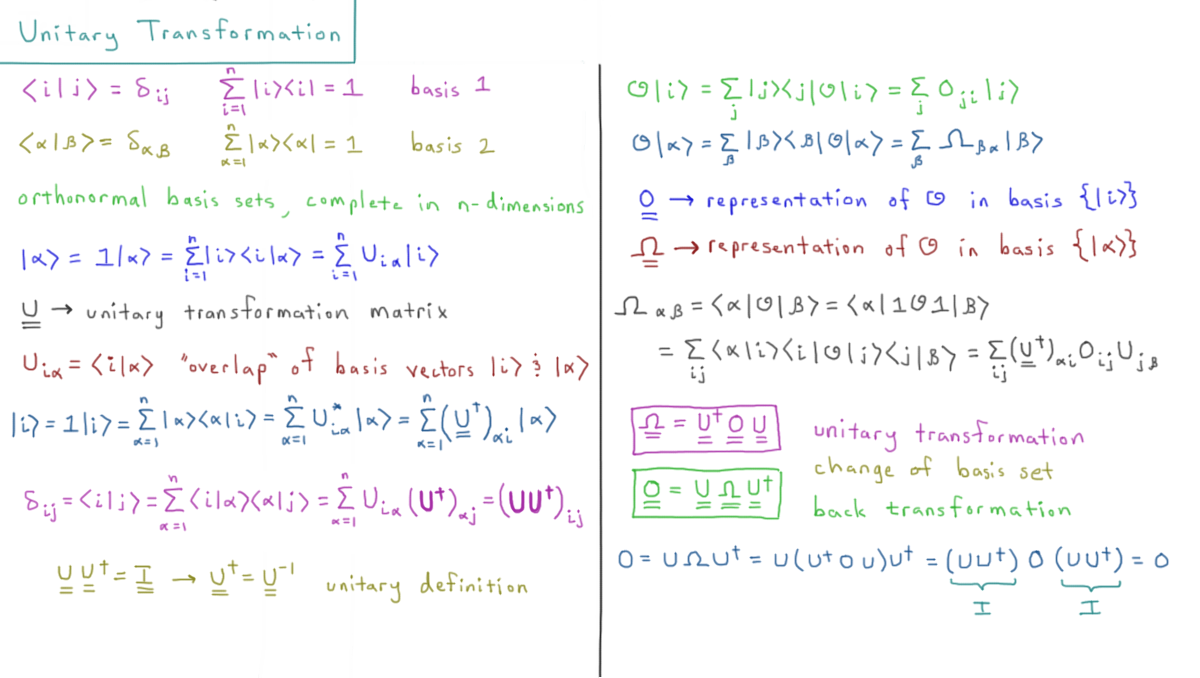
\includegraphics[width=1.2\textwidth]{./tmp_proc_img/Math/28.png}
\end{center}
}

\pagebreak[4]
\subsection{Hermitian Matrices}
\label{sec:org9449d34}
\makebox[\textwidth][c]{
\begin{center}
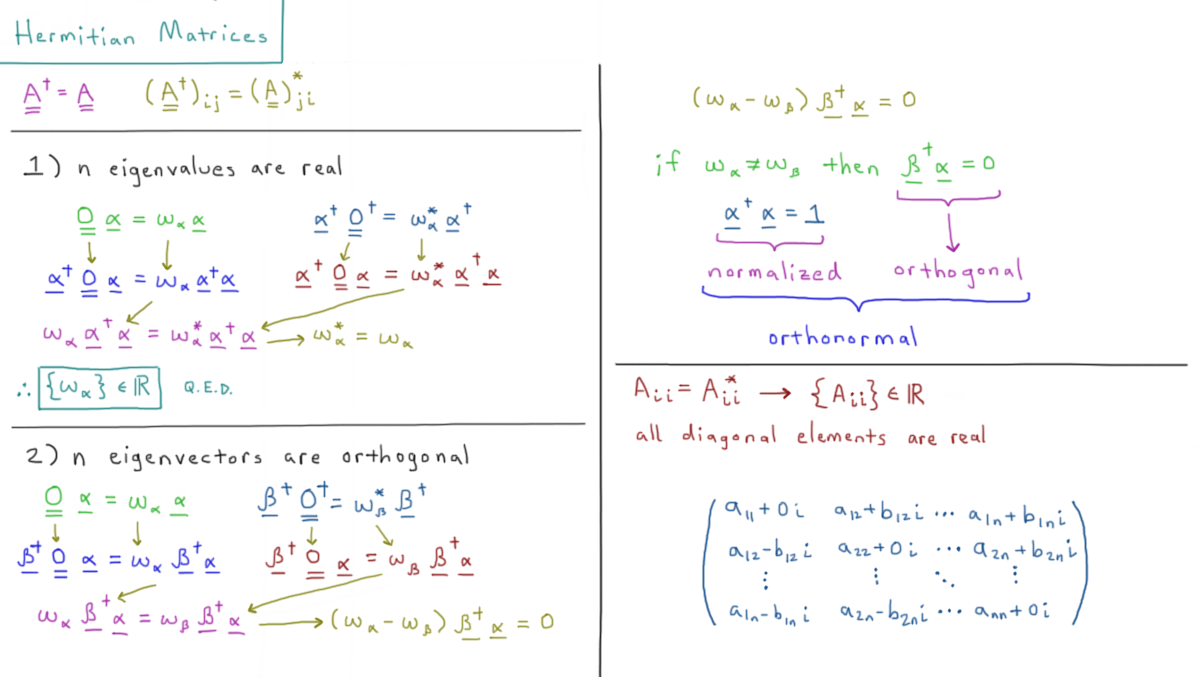
\includegraphics[width=1.2\textwidth]{./tmp_proc_img/Math/29.png}
\end{center}
}

\pagebreak[4]
\subsection{Matrix Diagonalization}
\label{sec:orgb240a51}
\makebox[\textwidth][c]{
\begin{center}
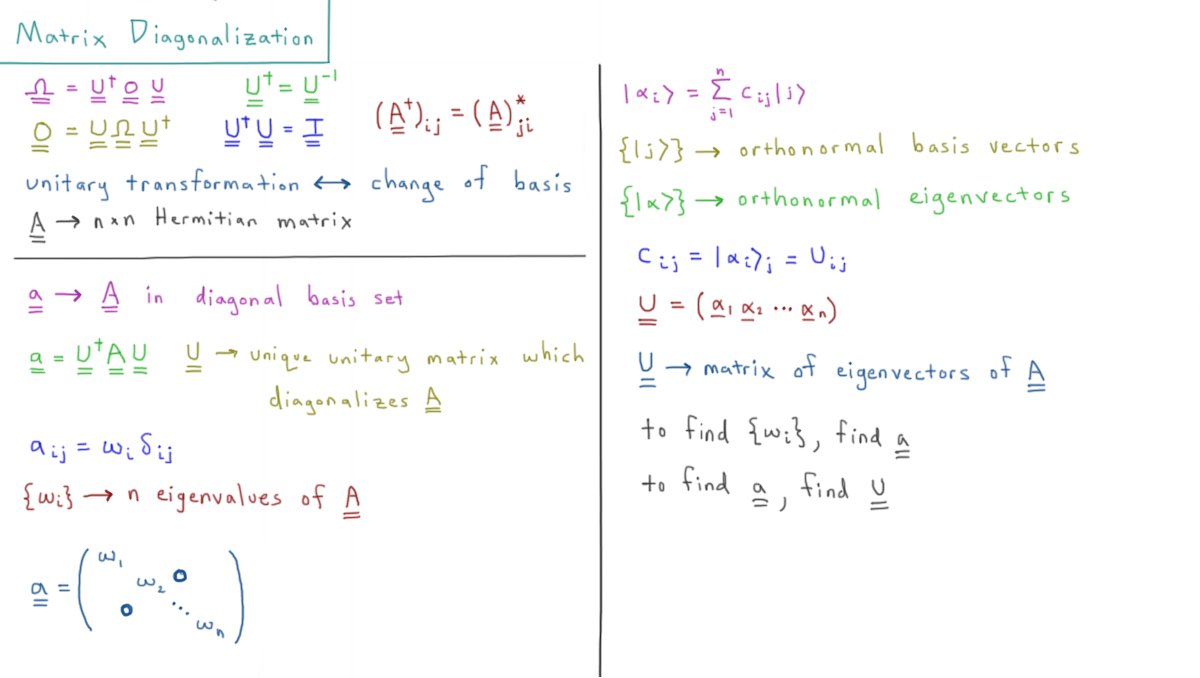
\includegraphics[width=1.2\textwidth]{./tmp_proc_img/Math/30.png}
\end{center}
}

\pagebreak[4]
\subsection{Matrix Commutators}
\label{sec:org4ad17d7}
\makebox[\textwidth][c]{
\begin{center}
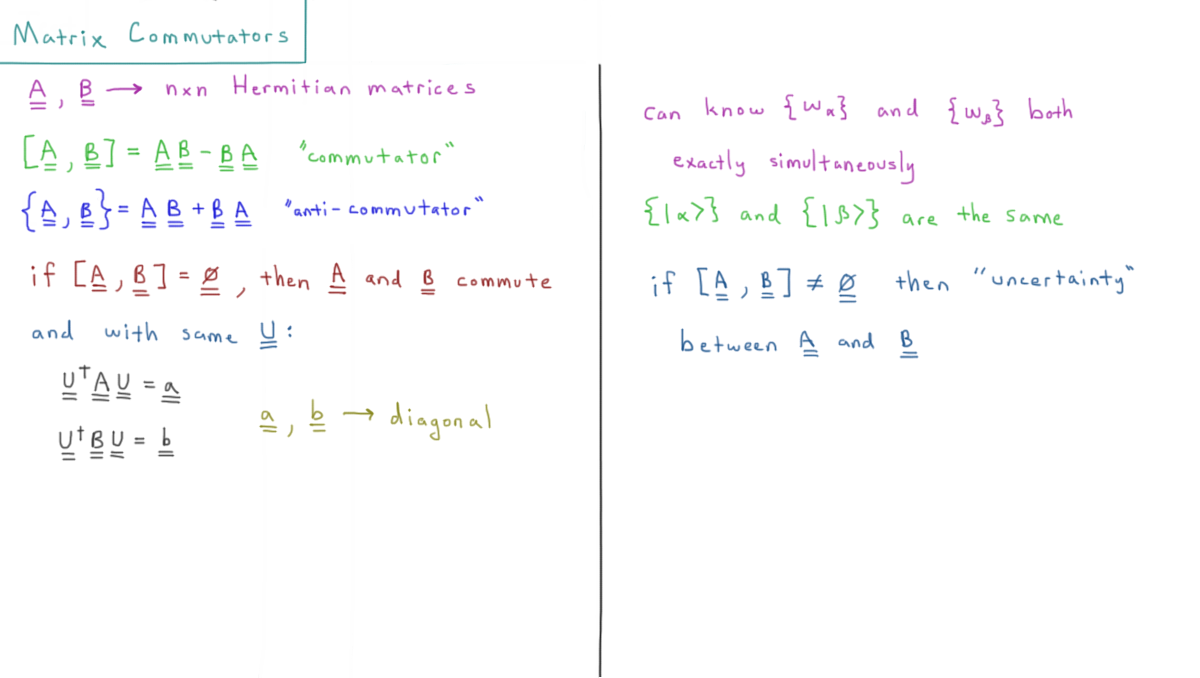
\includegraphics[width=1.2\textwidth]{./tmp_proc_img/Math/31.png}
\end{center}
}

\pagebreak[4]
\subsection{Matrix Functions}
\label{sec:orgc8aa514}
\makebox[\textwidth][c]{
\begin{center}
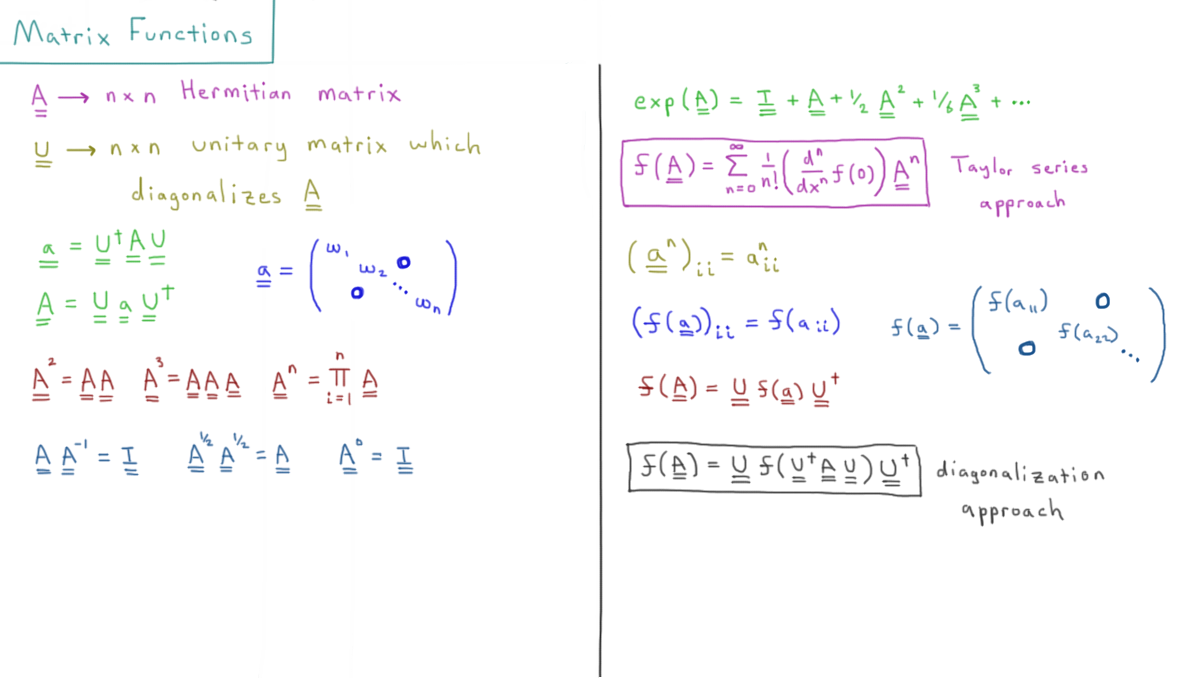
\includegraphics[width=1.2\textwidth]{./tmp_proc_img/Math/32.png}
\end{center}
}

\pagebreak[4]

\section{Quantum Chemistry }
\secttoc \pagebreak[4]
\label{sec:org26bf914}
\subsection{Introduction}
\label{sec:orgc800f1c}
\makebox[\textwidth][c]{
\begin{center}
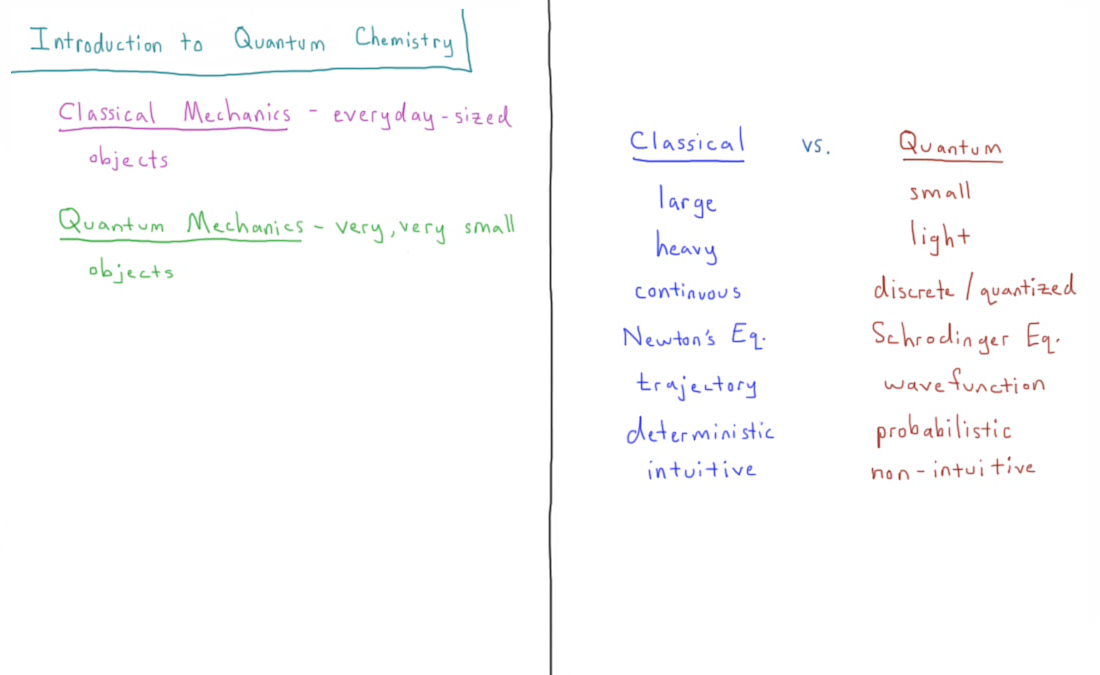
\includegraphics[width=1.2\textwidth]{./tmp_proc_img/quantum/0.png}
\end{center}
}

\pagebreak[4]
\subsection{Blackbody Radiation}
\label{sec:orgd5cfb5b}
\makebox[\textwidth][c]{
\begin{center}
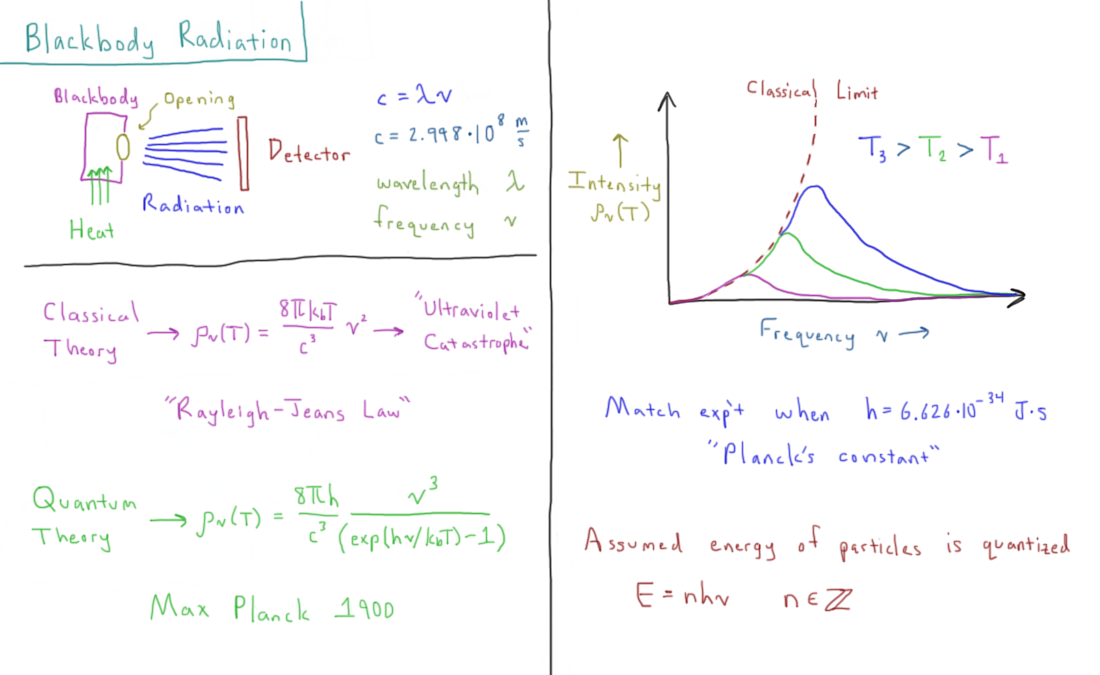
\includegraphics[width=1.2\textwidth]{./tmp_proc_img/quantum/1.png}
\end{center}
}

\pagebreak[4]
\subsection{Photoelectric Effect}
\label{sec:org5cc1765}
\makebox[\textwidth][c]{
\begin{center}
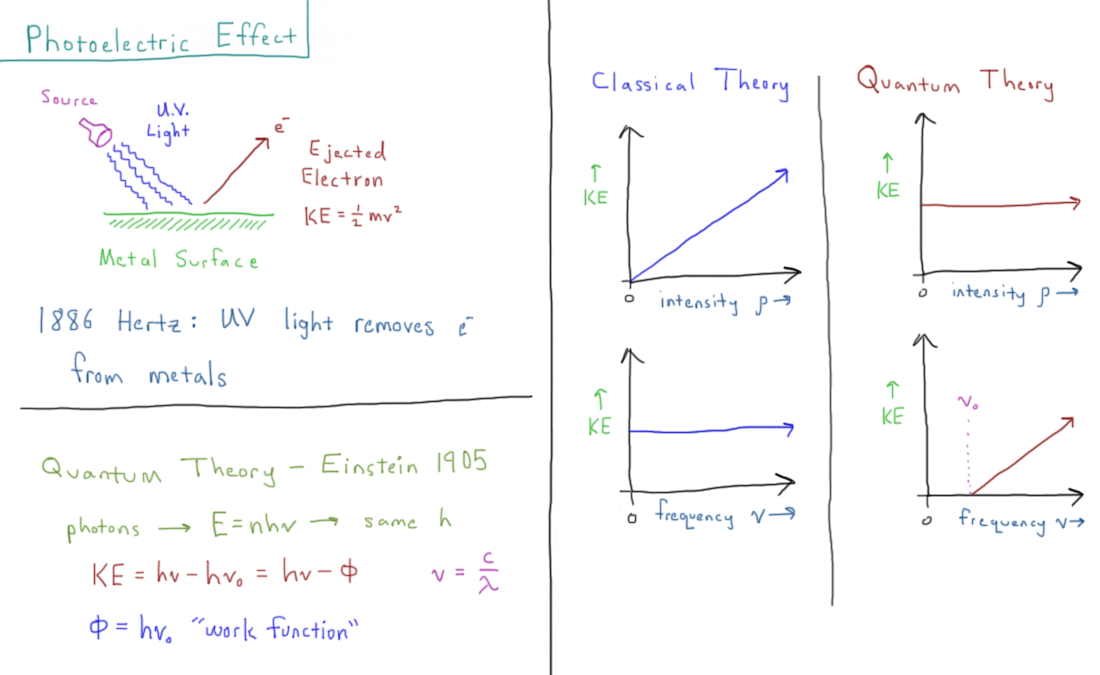
\includegraphics[width=1.2\textwidth]{./tmp_proc_img/quantum/2.png}
\end{center}
}

\pagebreak[4]
\subsection{Rydberg Formula}
\label{sec:org6ae0daa}
\makebox[\textwidth][c]{
\begin{center}
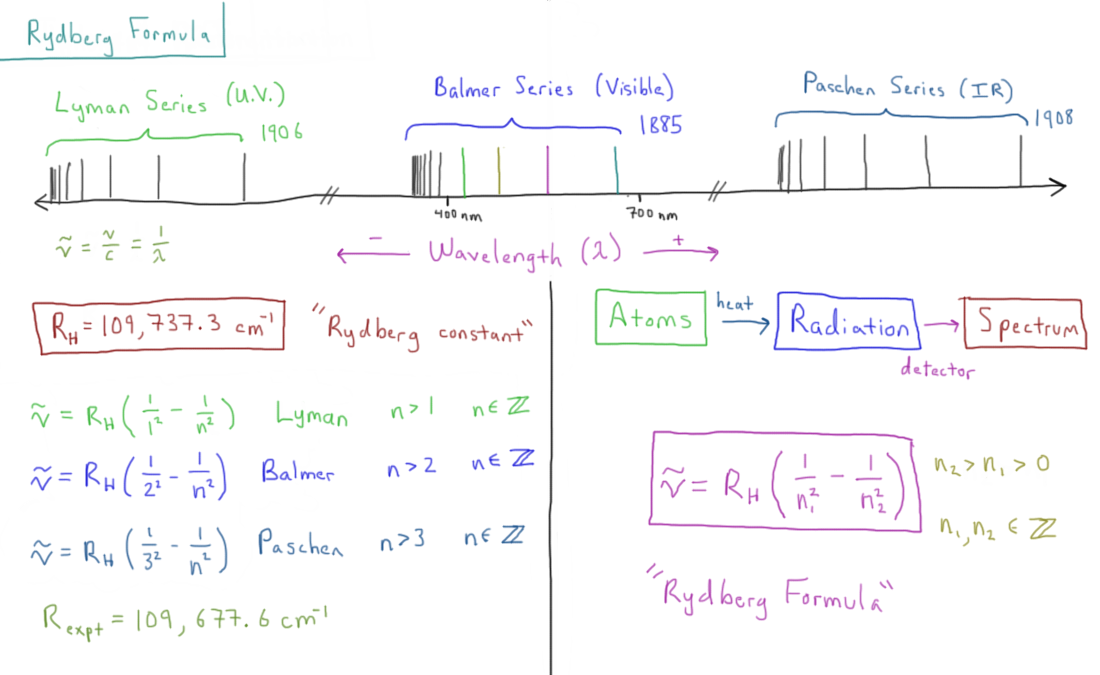
\includegraphics[width=1.2\textwidth]{./tmp_proc_img/quantum/3.png}
\end{center}
}

\pagebreak[4]
\subsection{Bohr Hydrogen Model 1: Radius}
\label{sec:org72c995d}
\makebox[\textwidth][c]{
\begin{center}
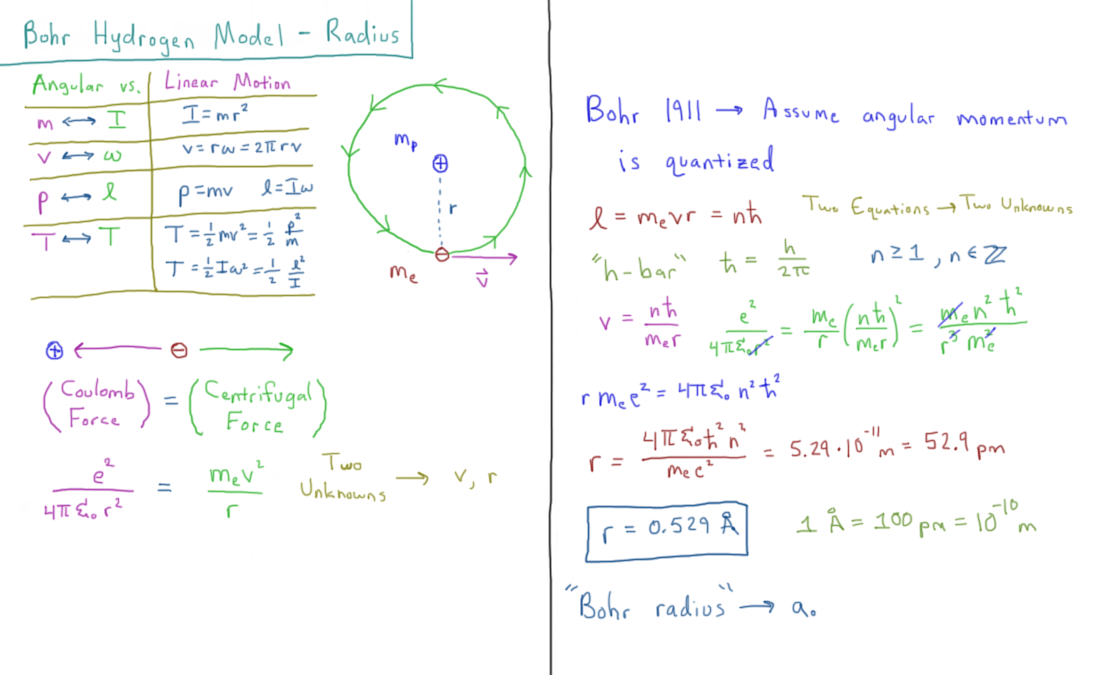
\includegraphics[width=1.2\textwidth]{./tmp_proc_img/quantum/4.png}
\end{center}
}

\pagebreak[4]
\subsection{Bohr Hydrogen Model 2: Energy}
\label{sec:org44a631d}
\makebox[\textwidth][c]{
\begin{center}
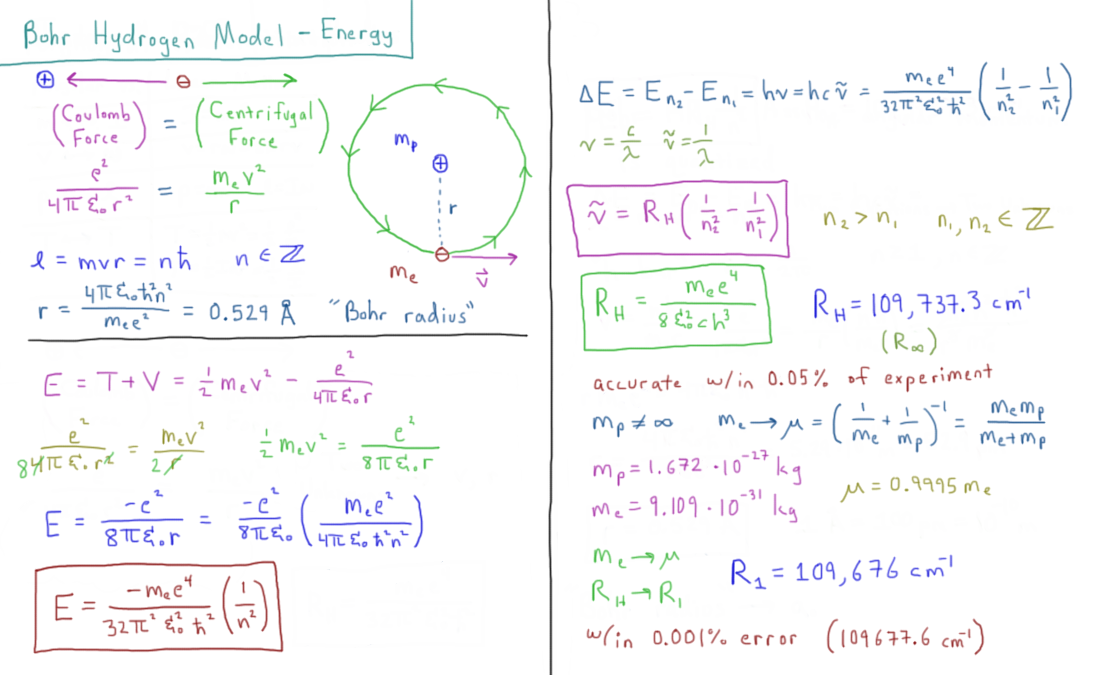
\includegraphics[width=1.2\textwidth]{./tmp_proc_img/quantum/5.png}
\end{center}
}

\pagebreak[4]
\subsection{Wave-Particle Duality}
\label{sec:orgd09571c}
\makebox[\textwidth][c]{
\begin{center}
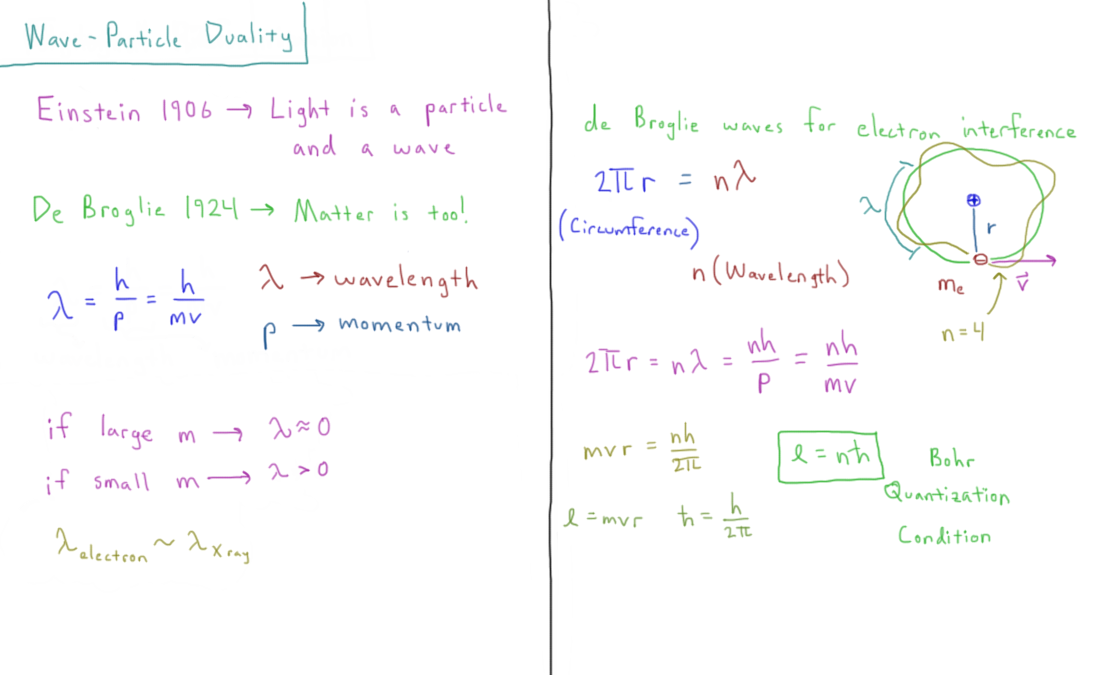
\includegraphics[width=1.2\textwidth]{./tmp_proc_img/quantum/6.png}
\end{center}
}

\pagebreak[4]
\subsection{Uncertainty Principle in Measurement}
\label{sec:orgc0af9a2}
\makebox[\textwidth][c]{
\begin{center}
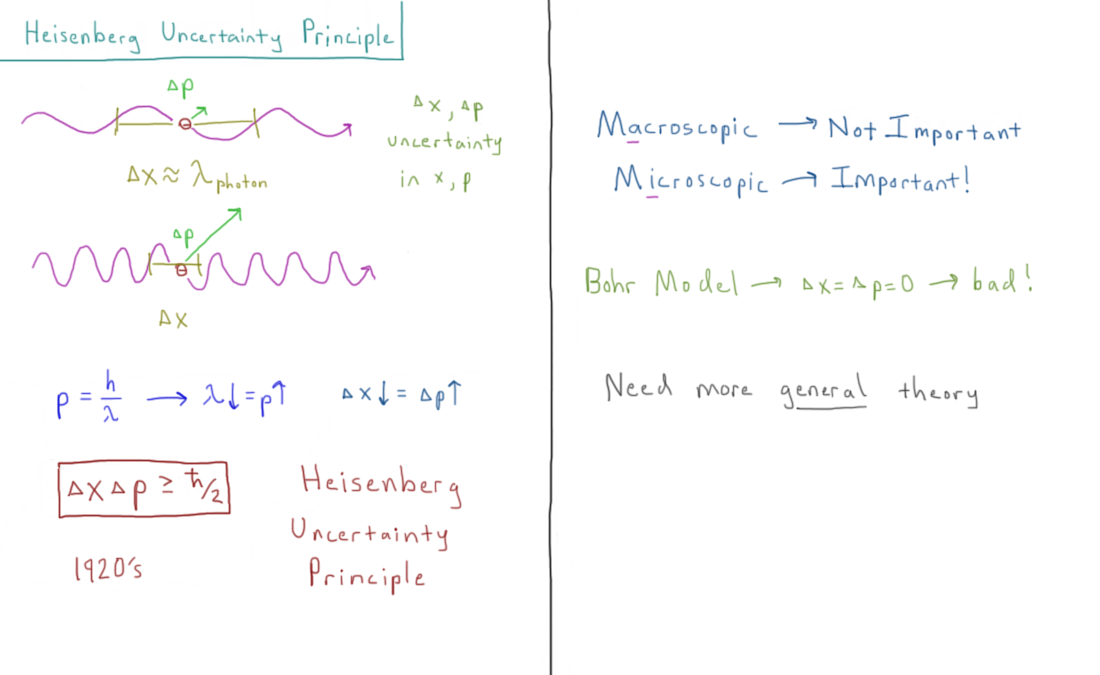
\includegraphics[width=1.2\textwidth]{./tmp_proc_img/quantum/7.png}
\end{center}
}

\pagebreak[4]
\subsection{Classical Wave Equation}
\label{sec:org5f6a045}
\makebox[\textwidth][c]{
\begin{center}
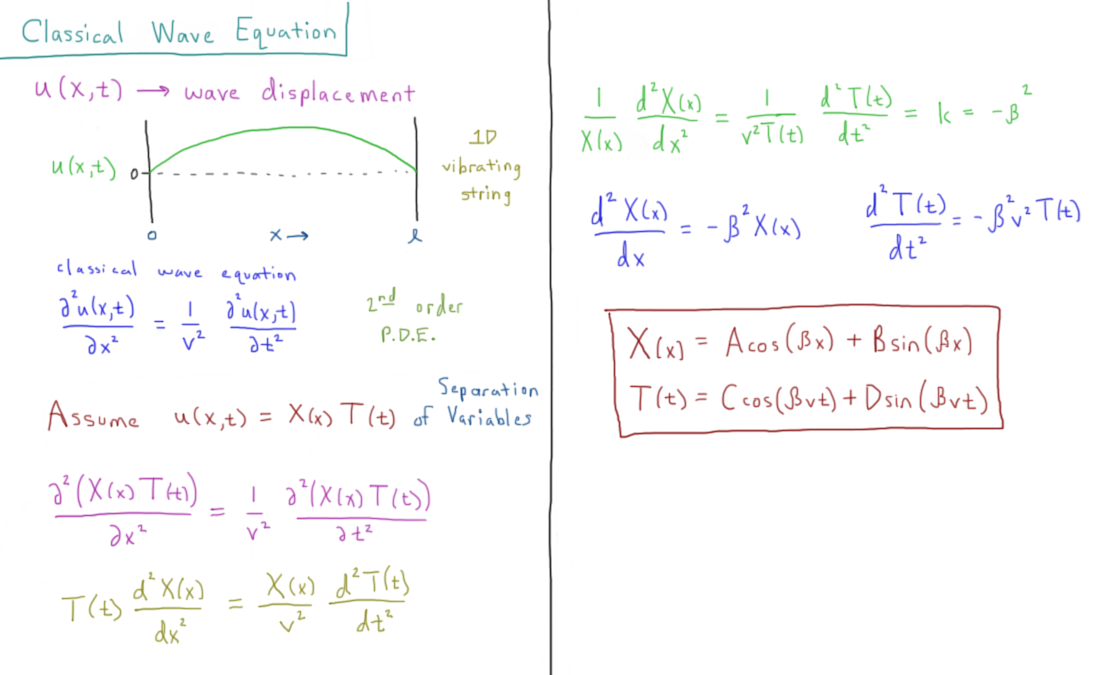
\includegraphics[width=1.2\textwidth]{./tmp_proc_img/quantum/8.png}
\end{center}
}

\pagebreak[4]
\subsection{Vibrating String}
\label{sec:org40b6e95}
\makebox[\textwidth][c]{
\begin{center}
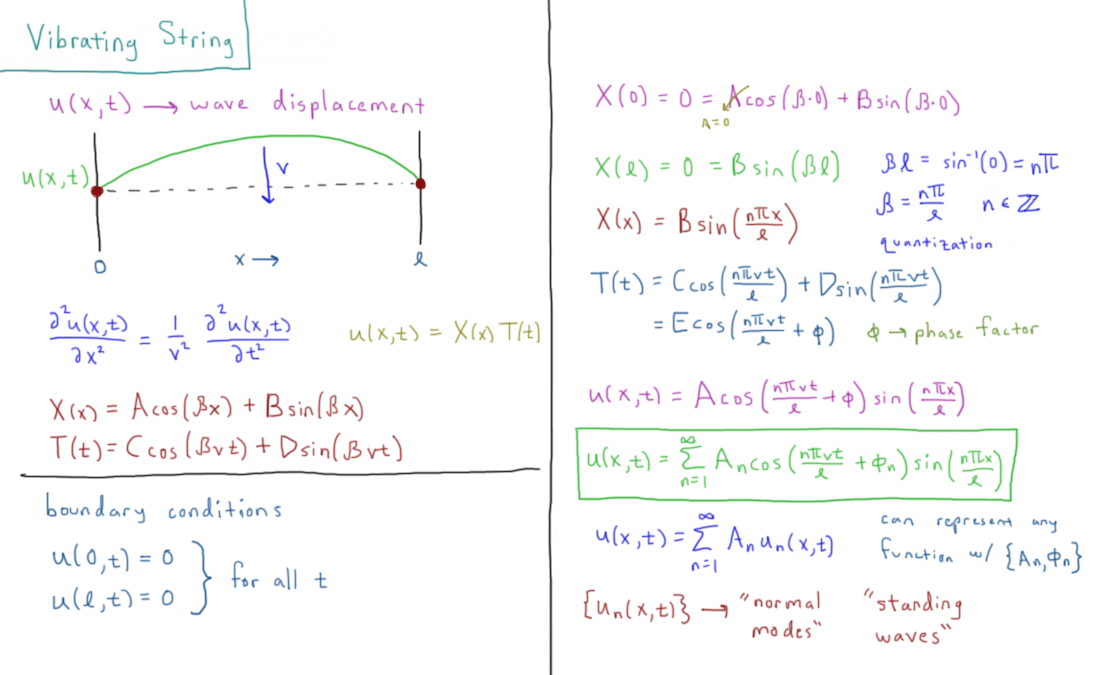
\includegraphics[width=1.2\textwidth]{./tmp_proc_img/quantum/9.png}
\end{center}
}

\pagebreak[4]
\subsection{Vibrating String Animation}
\label{sec:org113d79d}
\makebox[\textwidth][c]{
\begin{center}

\includegraphics[width=1.2\textwidth]{./tmp_proc_img/quantum/10.png}
\end{center}
}

\pagebreak[4]
\subsection{Schrodinger Equation "Derivation"}
\label{sec:orgf8b6013}
\makebox[\textwidth][c]{
\begin{center}
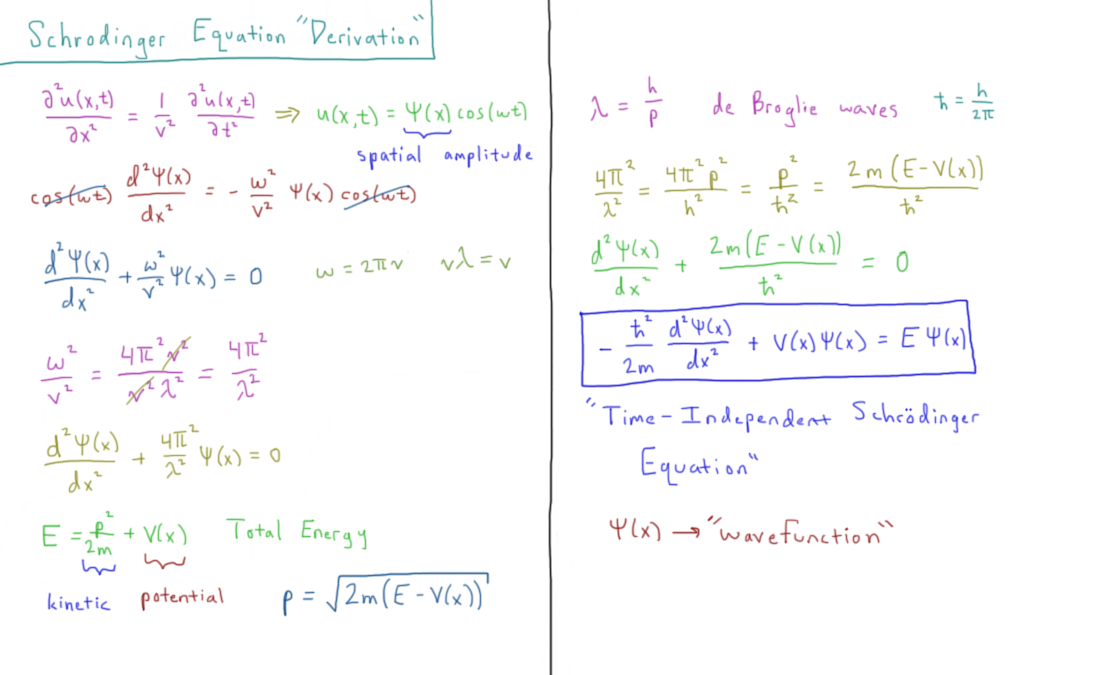
\includegraphics[width=1.2\textwidth]{./tmp_proc_img/quantum/11.png}
\end{center}
}

\pagebreak[4]
\subsection{Operators}
\label{sec:org3be05db}
\makebox[\textwidth][c]{
\begin{center}
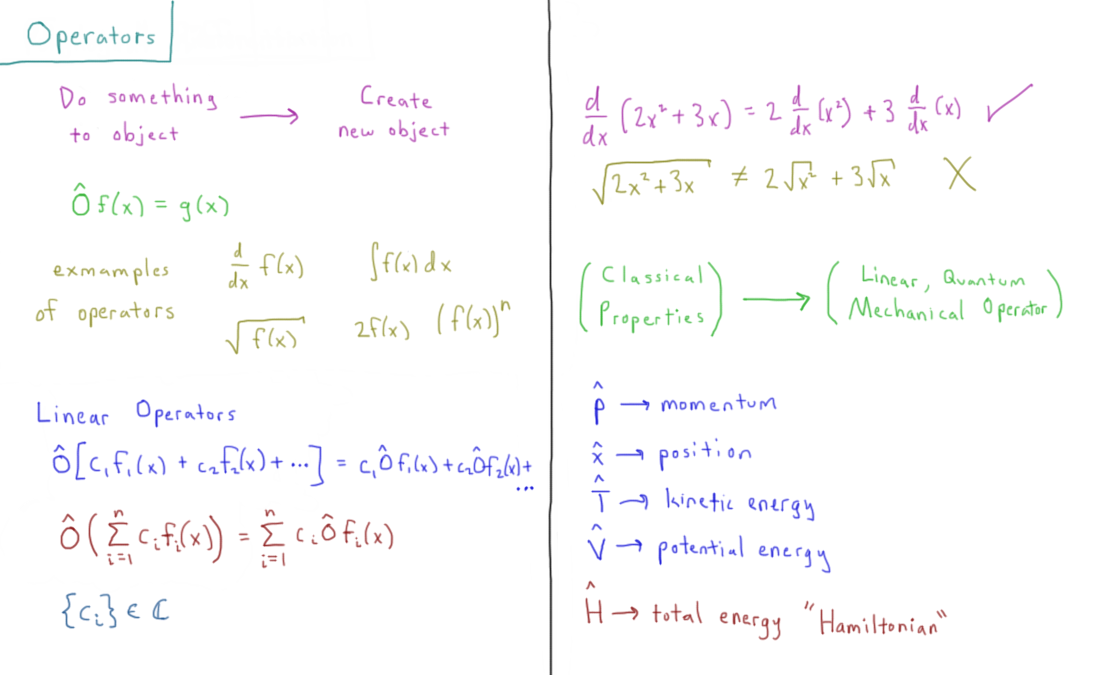
\includegraphics[width=1.2\textwidth]{./tmp_proc_img/quantum/12.png}
\end{center}
}

\pagebreak[4]
\subsection{Eigenvalues and Eigenfunctions}
\label{sec:org79cb252}
\makebox[\textwidth][c]{
\begin{center}
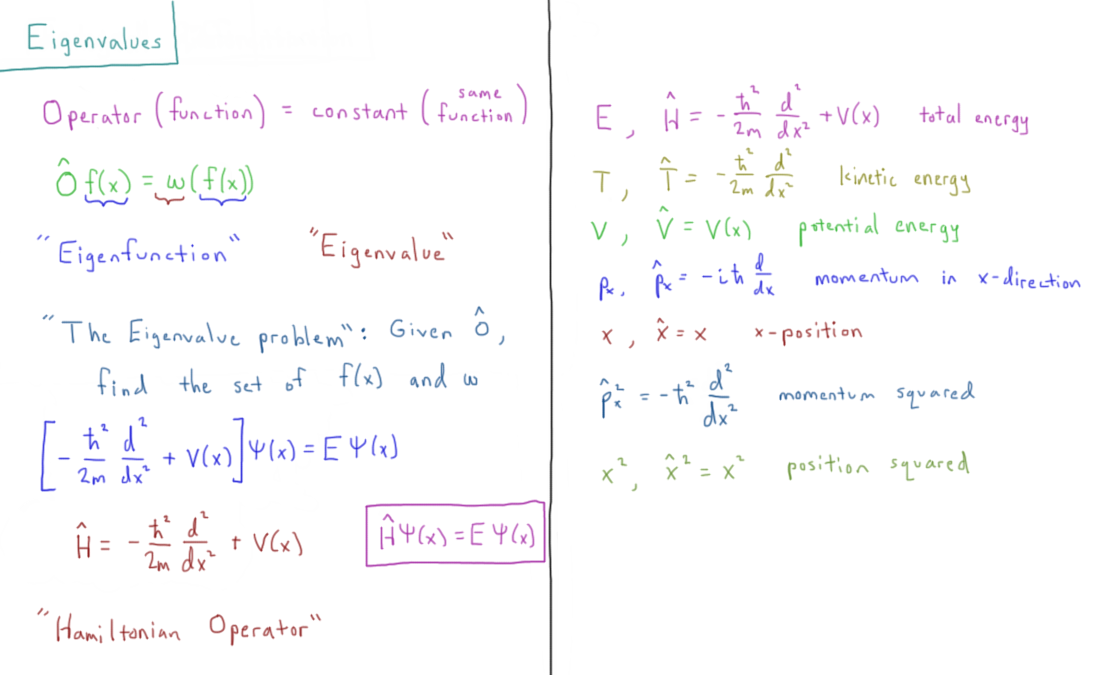
\includegraphics[width=1.2\textwidth]{./tmp_proc_img/quantum/13.png}
\end{center}
}

\pagebreak[4]
\subsection{Interpreting the Wavefunction}
\label{sec:org8ecd94a}
\makebox[\textwidth][c]{
\begin{center}
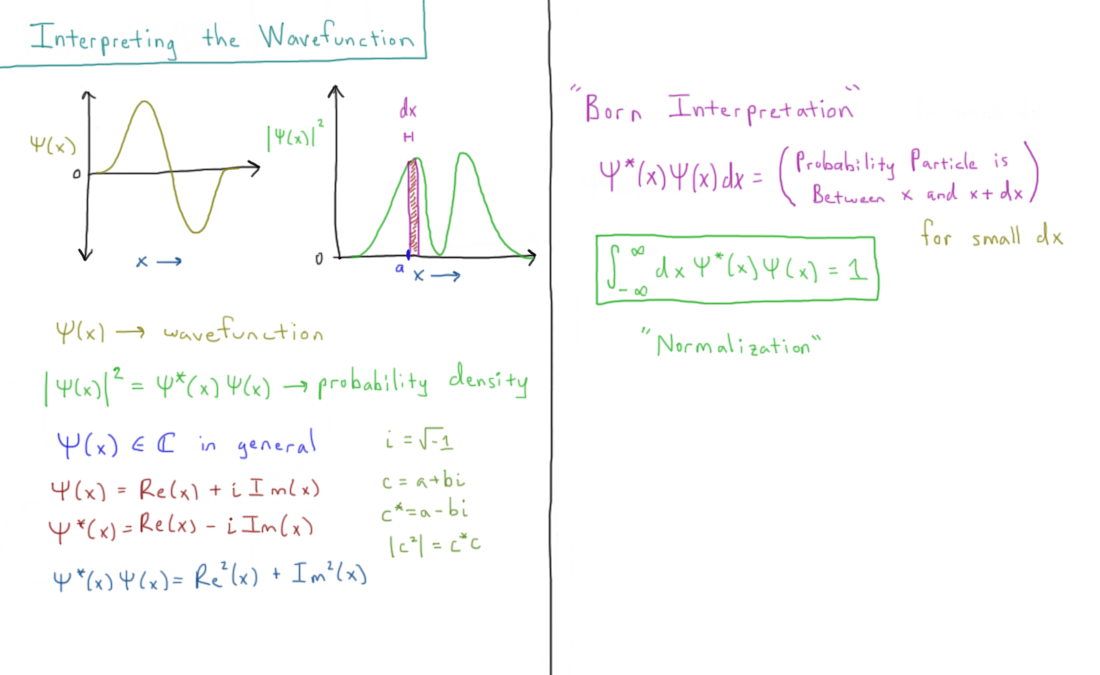
\includegraphics[width=1.2\textwidth]{./tmp_proc_img/quantum/14.png}
\end{center}
}

\pagebreak[4]
\subsection{Particle in a Box}
\label{sec:org4d325c7}
\makebox[\textwidth][c]{
\begin{center}
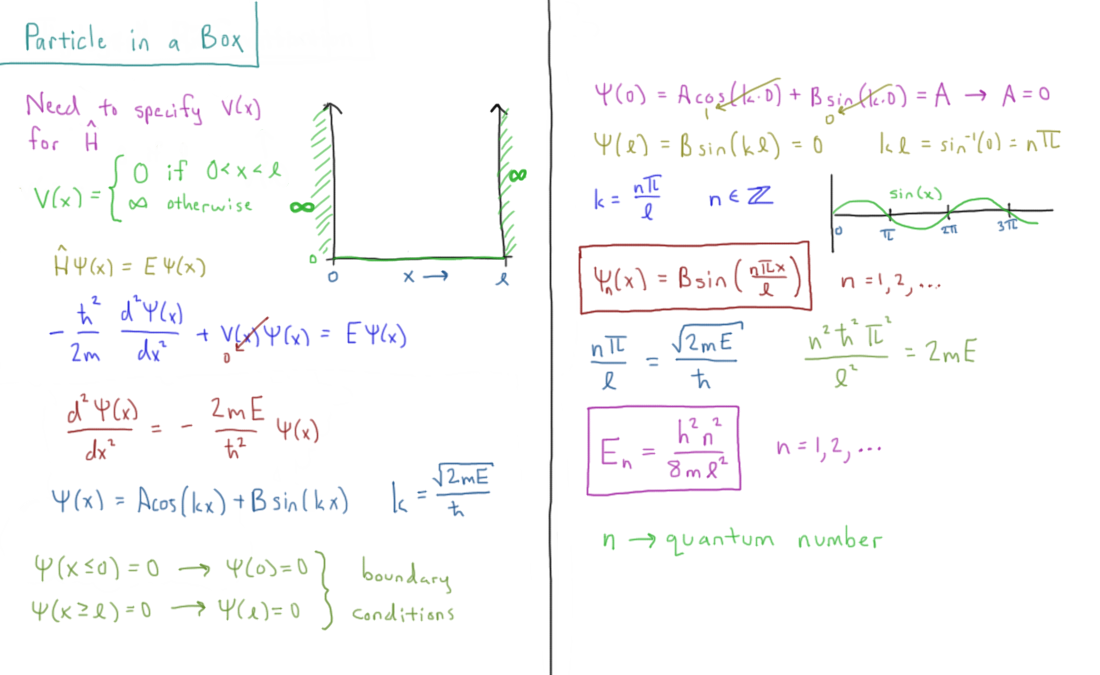
\includegraphics[width=1.2\textwidth]{./tmp_proc_img/quantum/15.png}
\end{center}
}

\pagebreak[4]
\subsection{Normalization}
\label{sec:org16b2b7b}
\makebox[\textwidth][c]{
\begin{center}
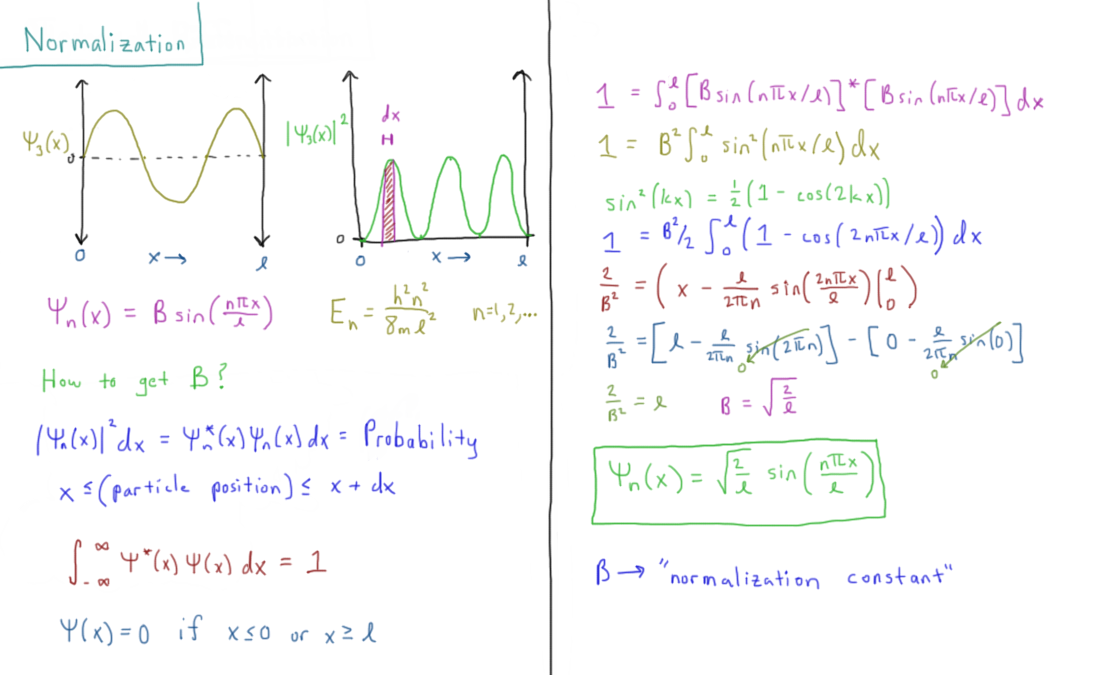
\includegraphics[width=1.2\textwidth]{./tmp_proc_img/quantum/16.png}
\end{center}
}

\pagebreak[4]
\subsection{Particle in a Box Wavefunction Plots}
\label{sec:orgadd996a}
\makebox[\textwidth][c]{
\begin{center}
\includegraphics[width=1.2\textwidth]{./tmp_proc_img/quantum/17.png}
\end{center}
}

\pagebreak[4]
\subsection{UV-Vis Spectra of Polyenes}
\label{sec:org9348ee8}
\makebox[\textwidth][c]{
\begin{center}
\includegraphics[width=1.2\textwidth]{./tmp_proc_img/quantum/18.png}
\end{center}
}

\pagebreak[4]
\subsection{Average Position}
\label{sec:org857a414}
\makebox[\textwidth][c]{
\begin{center}
\includegraphics[width=1.2\textwidth]{./tmp_proc_img/quantum/19.png}
\end{center}
}

\pagebreak[4]
\subsection{Average Momentum}
\label{sec:org6684e5d}
\makebox[\textwidth][c]{
\begin{center}
\includegraphics[width=1.2\textwidth]{./tmp_proc_img/quantum/20.png}
\end{center}
}

\pagebreak[4]
\subsection{3-D Particle in a Box}
\label{sec:orgf06c1e8}
\makebox[\textwidth][c]{
\begin{center}
\includegraphics[width=1.2\textwidth]{./tmp_proc_img/quantum/21.png}
\end{center}
}

\pagebreak[4]
\subsection{Degeneracy}
\label{sec:org8d513b8}
\makebox[\textwidth][c]{
\begin{center}
\includegraphics[width=1.2\textwidth]{./tmp_proc_img/quantum/22.png}
\end{center}
}

\pagebreak[4]
\subsection{Postulates of Quantum Mechanics 1: Wavefunction}
\label{sec:org3d88c63}
\makebox[\textwidth][c]{
\begin{center}
\includegraphics[width=1.2\textwidth]{./tmp_proc_img/quantum/23.png}
\end{center}
}

\pagebreak[4]
\subsection{Postulates of Quantum Mechanics 2: Operators}
\label{sec:orga087c29}
\makebox[\textwidth][c]{
\begin{center}
\includegraphics[width=1.2\textwidth]{./tmp_proc_img/quantum/24.png}
\end{center}
}

\pagebreak[4]
\subsection{Postulates of Quantum Mechanics 3: Measurement}
\label{sec:org1b0ce86}
\makebox[\textwidth][c]{
\begin{center}
\includegraphics[width=1.2\textwidth]{./tmp_proc_img/quantum/25.png}
\end{center}
}

\pagebreak[4]
\subsection{Postulates of Quantum Mechanics 4: Expectation Values}
\label{sec:org02996ee}
\makebox[\textwidth][c]{
\begin{center}
\includegraphics[width=1.2\textwidth]{./tmp_proc_img/quantum/26.png}
\end{center}
}

\pagebreak[4]
\subsection{Postulates of Quantum Mechanics 5: Schrodinger Equation}
\label{sec:org5096542}
\makebox[\textwidth][c]{
\begin{center}
\includegraphics[width=1.2\textwidth]{./tmp_proc_img/quantum/27.png}
\end{center}
}

\pagebreak[4]
\subsection{Commutators}
\label{sec:orga3985d6}
\makebox[\textwidth][c]{
\begin{center}
\includegraphics[width=1.2\textwidth]{./tmp_proc_img/quantum/28.png}
\end{center}
}

\pagebreak[4]
\subsection{Hermitian Operators}
\label{sec:org2b321c1}
\makebox[\textwidth][c]{
\begin{center}
\includegraphics[width=1.2\textwidth]{./tmp_proc_img/quantum/29.png}
\end{center}
}

\pagebreak[4]
\subsection{Dirac Notation}
\label{sec:org324c209}
\makebox[\textwidth][c]{
\begin{center}
\includegraphics[width=1.2\textwidth]{./tmp_proc_img/quantum/30.png}
\end{center}
}

\pagebreak[4]
\subsection{Orthogonality}
\label{sec:orga20545a}
\makebox[\textwidth][c]{
\begin{center}
\includegraphics[width=1.2\textwidth]{./tmp_proc_img/quantum/31.png}
\end{center}
}

\pagebreak[4]
\subsection{Superposition Principle 1: Basis Sets}
\label{sec:org05010a3}
\makebox[\textwidth][c]{
\begin{center}
\includegraphics[width=1.2\textwidth]{./tmp_proc_img/quantum/32.png}
\end{center}
}

\pagebreak[4]
\subsection{Superposition Principle 2: Expectation Values}
\label{sec:orgad22942}
\makebox[\textwidth][c]{
\begin{center}
\includegraphics[width=1.2\textwidth]{./tmp_proc_img/quantum/33.png}
\end{center}
}

\pagebreak[4]
\subsection{Superposition Principle 3: Example}
\label{sec:orgaa9d324}
\makebox[\textwidth][c]{
\begin{center}
\includegraphics[width=1.2\textwidth]{./tmp_proc_img/quantum/34.png}
\end{center}
}

\pagebreak[4]
\subsection{Commuting Operators}
\label{sec:org1ec968a}
\makebox[\textwidth][c]{
\begin{center}
\includegraphics[width=1.2\textwidth]{./tmp_proc_img/quantum/35.png}
\end{center}
}

\pagebreak[4]
\subsection{Time Dependence}
\label{sec:orgfd7dc92}
\makebox[\textwidth][c]{
\begin{center}
\includegraphics[width=1.2\textwidth]{./tmp_proc_img/quantum/36.png}
\end{center}
}

\pagebreak[4]
\subsection{Time Dependence Animation}
\label{sec:orge431fa1}
\makebox[\textwidth][c]{
\begin{center}
\includegraphics[width=1.2\textwidth]{./tmp_proc_img/quantum/37.png}
\end{center}
}

\pagebreak[4]
\subsection{Wavefunction Collapse}
\label{sec:org3e238a9}
\makebox[\textwidth][c]{
\begin{center}
\includegraphics[width=1.2\textwidth]{./tmp_proc_img/quantum/38.png}
\end{center}
}

\pagebreak[4]
\subsection{Schrodinger's Cat}
\label{sec:org7d617c3}
\makebox[\textwidth][c]{
\begin{center}
\includegraphics[width=1.2\textwidth]{./tmp_proc_img/quantum/39.png}
\end{center}
}

\pagebreak[4]
\subsection{Correspondence Principle}
\label{sec:org06df868}
\makebox[\textwidth][c]{
\begin{center}
\includegraphics[width=1.2\textwidth]{./tmp_proc_img/quantum/40.png}
\end{center}
}

\pagebreak[4]
\subsection{Harmonic Oscillator Model}
\label{sec:org38d424e}
\makebox[\textwidth][c]{
\begin{center}
\includegraphics[width=1.2\textwidth]{./tmp_proc_img/quantum/41.png}
\end{center}
}

\pagebreak[4]
\subsection{Classical Harmonic Oscillator 1: Trajectory}
\label{sec:orgcb3eb44}
\makebox[\textwidth][c]{
\begin{center}
\includegraphics[width=1.2\textwidth]{./tmp_proc_img/quantum/42.png}
\end{center}
}

\pagebreak[4]
\subsection{Classical Harmonic Oscillator 2: Energy}
\label{sec:org573cf4e}
\makebox[\textwidth][c]{
\begin{center}
\includegraphics[width=1.2\textwidth]{./tmp_proc_img/quantum/43.png}
\end{center}
}

\pagebreak[4]
\subsection{Reduced Mass}
\label{sec:orgf163533}
\makebox[\textwidth][c]{
\begin{center}
\includegraphics[width=1.2\textwidth]{./tmp_proc_img/quantum/44.png}
\end{center}
}

\pagebreak[4]
\subsection{Harmonic Oscillator Energy Levels}
\label{sec:org053b9ab}
\makebox[\textwidth][c]{
\begin{center}
\includegraphics[width=1.2\textwidth]{./tmp_proc_img/quantum/45.png}
\end{center}
}

\pagebreak[4]
\subsection{Diatomic Infrared Spectra}
\label{sec:org52dea38}
\makebox[\textwidth][c]{
\begin{center}
\includegraphics[width=1.2\textwidth]{./tmp_proc_img/quantum/46.png}
\end{center}
}

\pagebreak[4]
\subsection{Anharmonicity and Overtones}
\label{sec:orga9bbdd6}
\makebox[\textwidth][c]{
\begin{center}
\includegraphics[width=1.2\textwidth]{./tmp_proc_img/quantum/47.png}
\end{center}
}

\pagebreak[4]
\subsection{Harmonic Oscillator Wavefunctions}
\label{sec:orgec9abe3}
\makebox[\textwidth][c]{
\begin{center}
\includegraphics[width=1.2\textwidth]{./tmp_proc_img/quantum/48.png}
\end{center}
}

\pagebreak[4]
\subsection{Even and Odd Functions}
\label{sec:orgcb00d22}
\makebox[\textwidth][c]{
\begin{center}
\includegraphics[width=1.2\textwidth]{./tmp_proc_img/quantum/49.png}
\end{center}
}

\pagebreak[4]
\subsection{Harmonic Oscillator Even and Odd Functions}
\label{sec:org60041e3}
\makebox[\textwidth][c]{
\begin{center}
\includegraphics[width=1.2\textwidth]{./tmp_proc_img/quantum/50.png}
\end{center}
}

\pagebreak[4]
\subsection{3-D Harmonic Oscillator}
\label{sec:org0c4c6e4}
\makebox[\textwidth][c]{
\begin{center}
\includegraphics[width=1.2\textwidth]{./tmp_proc_img/quantum/51.png}
\end{center}
}

\pagebreak[4]
\subsection{Polyatomic Molecular Vibrations}
\label{sec:org0cae1cb}
\makebox[\textwidth][c]{
\begin{center}
\includegraphics[width=1.2\textwidth]{./tmp_proc_img/quantum/52.png}
\end{center}
}

\pagebreak[4]
\subsection{Rigid Rotor Model}
\label{sec:org9738ec4}
\makebox[\textwidth][c]{
\begin{center}
\includegraphics[width=1.2\textwidth]{./tmp_proc_img/quantum/53.png}
\end{center}
}

\pagebreak[4]
\subsection{Rotation Operators}
\label{sec:org4826d07}
\makebox[\textwidth][c]{
\begin{center}
\includegraphics[width=1.2\textwidth]{./tmp_proc_img/quantum/54.png}
\end{center}
}

\pagebreak[4]
\subsection{Rigid Rotor Energy Levels}
\label{sec:orga16edf0}
\makebox[\textwidth][c]{
\begin{center}
\includegraphics[width=1.2\textwidth]{./tmp_proc_img/quantum/55.png}
\end{center}
}

\pagebreak[4]
\subsection{Diatomic Microwave Spectra}
\label{sec:org3fdc8ca}
\makebox[\textwidth][c]{
\begin{center}
\includegraphics[width=1.2\textwidth]{./tmp_proc_img/quantum/56.png}
\end{center}
}

\pagebreak[4]
\subsection{Rovibrational Energy Levels}
\label{sec:org44c671f}
\makebox[\textwidth][c]{
\begin{center}
\includegraphics[width=1.2\textwidth]{./tmp_proc_img/quantum/57.png}
\end{center}
}

\pagebreak[4]
\subsection{Diatomic Rovibrational Spectra}
\label{sec:org6384d6c}
\makebox[\textwidth][c]{
\begin{center}
\includegraphics[width=1.2\textwidth]{./tmp_proc_img/quantum/58.png}
\end{center}
}

\pagebreak[4]
\subsection{Microwave Spectroscopy Example}
\label{sec:org63c8270}
\makebox[\textwidth][c]{
\begin{center}
\includegraphics[width=1.2\textwidth]{./tmp_proc_img/quantum/59.png}
\end{center}
}

\pagebreak[4]
\subsection{Rotation-Vibration Interaction}
\label{sec:orgc1a5272}
\makebox[\textwidth][c]{
\begin{center}
\includegraphics[width=1.2\textwidth]{./tmp_proc_img/quantum/60.png}
\end{center}
}

\pagebreak[4]
\subsection{Centrifugal Distortion}
\label{sec:org54023c0}
\makebox[\textwidth][c]{
\begin{center}
\includegraphics[width=1.2\textwidth]{./tmp_proc_img/quantum/61.png}
\end{center}
}

\pagebreak[4]
\subsection{Rigid Rotor Wavefunctions}
\label{sec:org9b7652c}
\makebox[\textwidth][c]{
\begin{center}
\includegraphics[width=1.2\textwidth]{./tmp_proc_img/quantum/62.png}
\end{center}
}

\pagebreak[4]
\subsection{Orthonormality of Spherical Harmonics}
\label{sec:org62f13a1}
\makebox[\textwidth][c]{
\begin{center}
\includegraphics[width=1.2\textwidth]{./tmp_proc_img/quantum/63.png}
\end{center}
}

\pagebreak[4]
\subsection{Angular Momentum Eigenvalues}
\label{sec:orge4b612e}
\makebox[\textwidth][c]{
\begin{center}
\includegraphics[width=1.2\textwidth]{./tmp_proc_img/quantum/64.png}
\end{center}
}

\pagebreak[4]
\subsection{Hydrogen Atom Model}
\label{sec:orgd86c483}
\makebox[\textwidth][c]{
\begin{center}
\includegraphics[width=1.2\textwidth]{./tmp_proc_img/quantum/65.png}
\end{center}
}

\pagebreak[4]
\subsection{Hydrogen Atom Energy Levels}
\label{sec:org2a98e7a}
\makebox[\textwidth][c]{
\begin{center}
\includegraphics[width=1.2\textwidth]{./tmp_proc_img/quantum/66.png}
\end{center}
}

\pagebreak[4]
\subsection{Hydrogen Atom Radial Wavefunctions}
\label{sec:orgc77dac8}
\makebox[\textwidth][c]{
\begin{center}
\includegraphics[width=1.2\textwidth]{./tmp_proc_img/quantum/67.png}
\end{center}
}

\pagebreak[4]
\subsection{Hydrogen Atom Total Wavefunctions}
\label{sec:orga4dcaad}
\makebox[\textwidth][c]{
\begin{center}
\includegraphics[width=1.2\textwidth]{./tmp_proc_img/quantum/68.png}
\end{center}
}

\pagebreak[4]
\subsection{Hydrogen Atomic Orbital Nodes}
\label{sec:org38d2631}
\makebox[\textwidth][c]{
\begin{center}
\includegraphics[width=1.2\textwidth]{./tmp_proc_img/quantum/69.png}
\end{center}
}

\pagebreak[4]
\subsection{Hydrogen Atom Eigenvalues}
\label{sec:org206d0be}
\makebox[\textwidth][c]{
\begin{center}
\includegraphics[width=1.2\textwidth]{./tmp_proc_img/quantum/70.png}
\end{center}
}

\pagebreak[4]
\subsection{Hydrogen Atom Radius}
\label{sec:org71b5d55}
\makebox[\textwidth][c]{
\begin{center}
\includegraphics[width=1.2\textwidth]{./tmp_proc_img/quantum/71.png}
\end{center}
}

\pagebreak[4]
\subsection{Hydrogen Atom Radial Wavefunction Animation}
\label{sec:org42d9897}
\makebox[\textwidth][c]{
\begin{center}
\includegraphics[width=1.2\textwidth]{./tmp_proc_img/quantum/72.png}
\end{center}
}

\pagebreak[4]
\subsection{Virial Theorem}
\label{sec:org1597f5e}
\makebox[\textwidth][c]{
\begin{center}
\includegraphics[width=1.2\textwidth]{./tmp_proc_img/quantum/73.png}
\end{center}
}

\pagebreak[4]
\subsection{Zeeman Effect}
\label{sec:org57043d7}
\makebox[\textwidth][c]{
\begin{center}
\includegraphics[width=1.2\textwidth]{./tmp_proc_img/quantum/74.png}
\end{center}
}

\pagebreak[4]
\subsection{Electron Spin}
\label{sec:org7546311}
\makebox[\textwidth][c]{
\begin{center}
\includegraphics[width=1.2\textwidth]{./tmp_proc_img/quantum/75.png}
\end{center}
}

\pagebreak[4]
\subsection{Spin-Orbit Coupling}
\label{sec:orgb25a28e}
\makebox[\textwidth][c]{
\begin{center}
\includegraphics[width=1.2\textwidth]{./tmp_proc_img/quantum/76.png}
\end{center}
}

\pagebreak[4]
\subsection{Hydrogen Atom Term Symbols}
\label{sec:org8090c4a}
\makebox[\textwidth][c]{
\begin{center}
\includegraphics[width=1.2\textwidth]{./tmp_proc_img/quantum/77.png}
\end{center}
}

\pagebreak[4]
\subsection{Hydrogen Atom Spectrum}
\label{sec:org222346f}
\makebox[\textwidth][c]{
\begin{center}
\includegraphics[width=1.2\textwidth]{./tmp_proc_img/quantum/78.png}
\end{center}
}

\pagebreak[4]
\subsection{Helium Atom Hamiltonian}
\label{sec:orgc3c1365}
\makebox[\textwidth][c]{
\begin{center}
\includegraphics[width=1.2\textwidth]{./tmp_proc_img/quantum/79.png}
\end{center}
}

\pagebreak[4]
\subsection{Variational Principle}
\label{sec:org84727ff}
\makebox[\textwidth][c]{
\begin{center}
\includegraphics[width=1.2\textwidth]{./tmp_proc_img/quantum/80.png}
\end{center}
}

\pagebreak[4]
\subsection{Variational Principle Example}
\label{sec:org46c710e}
\makebox[\textwidth][c]{
\begin{center}
\includegraphics[width=1.2\textwidth]{./tmp_proc_img/quantum/81.png}
\end{center}
}

\pagebreak[4]
\subsection{Linear Variational Method}
\label{sec:org2f6c98b}
\makebox[\textwidth][c]{
\begin{center}
\includegraphics[width=1.2\textwidth]{./tmp_proc_img/quantum/82.png}
\end{center}
}

\pagebreak[4]
\subsection{Secular Determinant}
\label{sec:orga46de87}
\makebox[\textwidth][c]{
\begin{center}
\includegraphics[width=1.2\textwidth]{./tmp_proc_img/quantum/83.png}
\end{center}
}

\pagebreak[4]
\subsection{Linear Variational Example}
\label{sec:orgfe79e5a}
\makebox[\textwidth][c]{
\begin{center}
\includegraphics[width=1.2\textwidth]{./tmp_proc_img/quantum/84.png}
\end{center}
}

\pagebreak[4]
\subsection{Perturbation Theory}
\label{sec:org154f7e6}
\makebox[\textwidth][c]{
\begin{center}
\includegraphics[width=1.2\textwidth]{./tmp_proc_img/quantum/85.png}
\end{center}
}

\pagebreak[4]
\subsection{Perturbation Theory Derivation}
\label{sec:orgf733e54}
\makebox[\textwidth][c]{
\begin{center}
\includegraphics[width=1.2\textwidth]{./tmp_proc_img/quantum/86.png}
\end{center}
}

\pagebreak[4]
\subsection{Perturbation Theory Example}
\label{sec:org2b4cb23}
\makebox[\textwidth][c]{
\begin{center}
\includegraphics[width=1.2\textwidth]{./tmp_proc_img/quantum/87.png}
\end{center}
}

\pagebreak[4]
\subsection{Atomic Units}
\label{sec:org15ea930}
\makebox[\textwidth][c]{
\begin{center}
\includegraphics[width=1.2\textwidth]{./tmp_proc_img/quantum/88.png}
\end{center}
}

\pagebreak[4]
\subsection{Helium Atom Energy Approximations}
\label{sec:org586e593}
\makebox[\textwidth][c]{
\begin{center}
\includegraphics[width=1.2\textwidth]{./tmp_proc_img/quantum/89.png}
\end{center}
}

\pagebreak[4]
\subsection{Hartree-Fock Helium Atom}
\label{sec:org63377c4}
\makebox[\textwidth][c]{
\begin{center}
\includegraphics[width=1.2\textwidth]{./tmp_proc_img/quantum/90.png}
\end{center}
}

\pagebreak[4]
\subsection{Hartree-Fock Helium Energy}
\label{sec:org571c346}
\makebox[\textwidth][c]{
\begin{center}
\includegraphics[width=1.2\textwidth]{./tmp_proc_img/quantum/91.png}
\end{center}
}

\pagebreak[4]
\subsection{Antisymmetry Principle}
\label{sec:orgf3a46f7}
\makebox[\textwidth][c]{
\begin{center}
\includegraphics[width=1.2\textwidth]{./tmp_proc_img/quantum/92.png}
\end{center}
}

\pagebreak[4]
\subsection{Slater Determinants}
\label{sec:orgd7e876e}
\makebox[\textwidth][c]{
\begin{center}
\includegraphics[width=1.2\textwidth]{./tmp_proc_img/quantum/93.png}
\end{center}
}

\pagebreak[4]
\subsection{Hartree-Fock Atomic Energy}
\label{sec:orgf4b2e12}
\makebox[\textwidth][c]{
\begin{center}
\includegraphics[width=1.2\textwidth]{./tmp_proc_img/quantum/94.png}
\end{center}
}

\pagebreak[4]
\subsection{Hartree-Fock Operators}
\label{sec:org3f51cd8}
\makebox[\textwidth][c]{
\begin{center}
\includegraphics[width=1.2\textwidth]{./tmp_proc_img/quantum/95.png}
\end{center}
}

\pagebreak[4]
\subsection{Hartree-Fock-Roothaan Equations}
\label{sec:org883772a}
\makebox[\textwidth][c]{
\begin{center}
\includegraphics[width=1.2\textwidth]{./tmp_proc_img/quantum/96.png}
\end{center}
}

\pagebreak[4]
\subsection{Hartree-Fock Spin}
\label{sec:org859ad66}
\makebox[\textwidth][c]{
\begin{center}
\includegraphics[width=1.2\textwidth]{./tmp_proc_img/quantum/97.png}
\end{center}
}

\pagebreak[4]
\subsection{Post Hartree-Fock Methods}
\label{sec:orgbab7024}
\makebox[\textwidth][c]{
\begin{center}
\includegraphics[width=1.2\textwidth]{./tmp_proc_img/quantum/98.png}
\end{center}
}

\pagebreak[4]
\subsection{Atomic Electron Configurations}
\label{sec:org7233cf3}
\makebox[\textwidth][c]{
\begin{center}
\includegraphics[width=1.2\textwidth]{./tmp_proc_img/quantum/99.png}
\end{center}
}

\pagebreak[4]
\subsection{Electron Configuration Exceptions}
\label{sec:org1f134df}
\makebox[\textwidth][c]{
\begin{center}
\includegraphics[width=1.2\textwidth]{./tmp_proc_img/quantum/100.png}
\end{center}
}

\pagebreak[4]
\subsection{Atomic Term Symbols}
\label{sec:org7207d0f}
\makebox[\textwidth][c]{
\begin{center}
\includegraphics[width=1.2\textwidth]{./tmp_proc_img/quantum/101.png}
\end{center}
}

\pagebreak[4]
\subsection{Term Symbols Example 1}
\label{sec:org891ca3c}
\makebox[\textwidth][c]{
\begin{center}
\includegraphics[width=1.2\textwidth]{./tmp_proc_img/quantum/102.png}
\end{center}
}

\pagebreak[4]
\subsection{Term Symbols Example 2}
\label{sec:orgb9c6899}
\makebox[\textwidth][c]{
\begin{center}
\includegraphics[width=1.2\textwidth]{./tmp_proc_img/quantum/103.png}
\end{center}
}

\pagebreak[4]
\subsection{Term Symbols Example 3}
\label{sec:org4609407}
\makebox[\textwidth][c]{
\begin{center}
\includegraphics[width=1.2\textwidth]{./tmp_proc_img/quantum/104.png}
\end{center}
}

\pagebreak[4]
\subsection{Hund's Rules}
\label{sec:org5d4d60f}
\makebox[\textwidth][c]{
\begin{center}
\includegraphics[width=1.2\textwidth]{./tmp_proc_img/quantum/105.png}
\end{center}
}

\pagebreak[4]
\subsection{Atomic Spectra}
\label{sec:org6c482bc}
\makebox[\textwidth][c]{
\begin{center}
\includegraphics[width=1.2\textwidth]{./tmp_proc_img/quantum/106.png}
\end{center}
}

\pagebreak[4]
\subsection{Hydrogen Molecule Hamiltonian}
\label{sec:org6a0190f}
\makebox[\textwidth][c]{
\begin{center}
\includegraphics[width=1.2\textwidth]{./tmp_proc_img/quantum/107.png}
\end{center}
}

\pagebreak[4]
\subsection{Born-Oppenheimer Approximation}
\label{sec:org43b3047}
\makebox[\textwidth][c]{
\begin{center}
\includegraphics[width=1.2\textwidth]{./tmp_proc_img/quantum/108.png}
\end{center}
}

\pagebreak[4]
\subsection{Hydrogen Molecule-Ion 1: Energy}
\label{sec:org652313c}
\makebox[\textwidth][c]{
\begin{center}
\includegraphics[width=1.2\textwidth]{./tmp_proc_img/quantum/109.png}
\end{center}
}

\pagebreak[4]
\subsection{Hydrogen Molecule-Ion 2: Orbitals}
\label{sec:orgc9b7e2c}
\makebox[\textwidth][c]{
\begin{center}
\includegraphics[width=1.2\textwidth]{./tmp_proc_img/quantum/110.png}
\end{center}
}

\pagebreak[4]
\subsection{Molecular Orbital Angular Momentum}
\label{sec:orgf427a1d}
\makebox[\textwidth][c]{
\begin{center}
\includegraphics[width=1.2\textwidth]{./tmp_proc_img/quantum/111.png}
\end{center}
}

\pagebreak[4]
\subsection{Molecular Orbital Inversion Symmetry}
\label{sec:org0fcecdf}
\makebox[\textwidth][c]{
\begin{center}
\includegraphics[width=1.2\textwidth]{./tmp_proc_img/quantum/112.png}
\end{center}
}

\pagebreak[4]
\subsection{Hydrogen Molecular Orbital Diagram}
\label{sec:orgcd28350}
\makebox[\textwidth][c]{
\begin{center}
\includegraphics[width=1.2\textwidth]{./tmp_proc_img/quantum/113.png}
\end{center}
}

\pagebreak[4]
\subsection{LCAO-MO Theory}
\label{sec:orgfeffef5}
\makebox[\textwidth][c]{
\begin{center}
\includegraphics[width=1.2\textwidth]{./tmp_proc_img/quantum/114.png}
\end{center}
}

\pagebreak[4]
\subsection{Diatomic Molecular Orbital Diagrams}
\label{sec:orgb8d8bee}
\makebox[\textwidth][c]{
\begin{center}
\includegraphics[width=1.2\textwidth]{./tmp_proc_img/quantum/115.png}
\end{center}
}

\pagebreak[4]
\subsection{Bond Order}
\label{sec:org9200669}
\makebox[\textwidth][c]{
\begin{center}
\includegraphics[width=1.2\textwidth]{./tmp_proc_img/quantum/116.png}
\end{center}
}

\pagebreak[4]
\subsection{Diatomic Term Symbols}
\label{sec:orga7eb09e}
\makebox[\textwidth][c]{
\begin{center}
\includegraphics[width=1.2\textwidth]{./tmp_proc_img/quantum/117.png}
\end{center}
}

\pagebreak[4]
\subsection{Total Wavefunction Symmetry}
\label{sec:orgda19413}
\makebox[\textwidth][c]{
\begin{center}
\includegraphics[width=1.2\textwidth]{./tmp_proc_img/quantum/118.png}
\end{center}
}

\pagebreak[4]
\subsection{sp Hybridization}
\label{sec:org74a20d1}
\makebox[\textwidth][c]{
\begin{center}
\includegraphics[width=1.2\textwidth]{./tmp_proc_img/quantum/119.png}
\end{center}
}

\pagebreak[4]
\subsection{sp2 Hybridization}
\label{sec:org8eb3d7c}
\makebox[\textwidth][c]{
\begin{center}
\includegraphics[width=1.2\textwidth]{./tmp_proc_img/quantum/120.png}
\end{center}
}

\pagebreak[4]
\subsection{sp3 Hybridization}
\label{sec:org39ca171}
\makebox[\textwidth][c]{
\begin{center}
\includegraphics[width=1.2\textwidth]{./tmp_proc_img/quantum/121.png}
\end{center}
}

\pagebreak[4]
\subsection{Lone Pair Hybridization}
\label{sec:org8de52a2}
\makebox[\textwidth][c]{
\begin{center}
\includegraphics[width=1.2\textwidth]{./tmp_proc_img/quantum/122.png}
\end{center}
}

\pagebreak[4]
\subsection{Walsh Diagrams}
\label{sec:org5d8640a}
\makebox[\textwidth][c]{
\begin{center}
\includegraphics[width=1.2\textwidth]{./tmp_proc_img/quantum/123.png}
\end{center}
}

\pagebreak[4]
\subsection{Huckel Theory}
\label{sec:org0927a8a}
\makebox[\textwidth][c]{
\begin{center}
\includegraphics[width=1.2\textwidth]{./tmp_proc_img/quantum/124.png}
\end{center}
}

\pagebreak[4]
\subsection{Pi Resonance}
\label{sec:orgae37c5f}
\makebox[\textwidth][c]{
\begin{center}
\includegraphics[width=1.2\textwidth]{./tmp_proc_img/quantum/125.png}
\end{center}
}

\pagebreak[4]
\subsection{Aromaticity}
\label{sec:org9534359}
\makebox[\textwidth][c]{
\begin{center}
\includegraphics[width=1.2\textwidth]{./tmp_proc_img/quantum/126.png}
\end{center}
}

\pagebreak[4]
\subsection{Symmetry Websites}
\label{sec:org606f34e}
\makebox[\textwidth][c]{
\begin{center}
\includegraphics[width=1.2\textwidth]{./tmp_proc_img/quantum/127.png}
\end{center}
}

\pagebreak[4]
\subsection{Symmetry Operations}
\label{sec:org184c784}
\makebox[\textwidth][c]{
\begin{center}
\includegraphics[width=1.2\textwidth]{./tmp_proc_img/quantum/128.png}
\end{center}
}

\pagebreak[4]
\subsection{Symmetry Elements}
\label{sec:org43239d6}
\makebox[\textwidth][c]{
\begin{center}
\includegraphics[width=1.2\textwidth]{./tmp_proc_img/quantum/129.png}
\end{center}
}

\pagebreak[4]
\subsection{Groups}
\label{sec:orgd860904}
\makebox[\textwidth][c]{
\begin{center}
\includegraphics[width=1.2\textwidth]{./tmp_proc_img/quantum/130.png}
\end{center}
}

\pagebreak[4]
\subsection{Point Groups}
\label{sec:orgbe3cc64}
\makebox[\textwidth][c]{
\begin{center}
\includegraphics[width=1.2\textwidth]{./tmp_proc_img/quantum/131.png}
\end{center}
}

\pagebreak[4]
\subsection{Point Group Examples}
\label{sec:org45f1a15}
\makebox[\textwidth][c]{
\begin{center}
\includegraphics[width=1.2\textwidth]{./tmp_proc_img/quantum/132.png}
\end{center}
}

\pagebreak[4]
\subsection{Determining Point Groups}
\label{sec:org132fcf1}
\makebox[\textwidth][c]{
\begin{center}
\includegraphics[width=1.2\textwidth]{./tmp_proc_img/quantum/133.png}
\end{center}
}

\pagebreak[4]
\subsection{Group Multiplication Tables}
\label{sec:org0eac690}
\makebox[\textwidth][c]{
\begin{center}
\includegraphics[width=1.2\textwidth]{./tmp_proc_img/quantum/134.png}
\end{center}
}

\pagebreak[4]
\subsection{Symmetry Operator Matrices}
\label{sec:orgae49a34}
\makebox[\textwidth][c]{
\begin{center}
\includegraphics[width=1.2\textwidth]{./tmp_proc_img/quantum/135.png}
\end{center}
}

\pagebreak[4]
\subsection{Irreducible Representations}
\label{sec:orge0a3b5b}
\makebox[\textwidth][c]{
\begin{center}
\includegraphics[width=1.2\textwidth]{./tmp_proc_img/quantum/136.png}
\end{center}
}

\pagebreak[4]
\subsection{Character Tables 1: Abelian}
\label{sec:org7e18a4c}
\makebox[\textwidth][c]{
\begin{center}
\includegraphics[width=1.2\textwidth]{./tmp_proc_img/quantum/137.png}
\end{center}
}

\pagebreak[4]
\subsection{Character Tables 2: Non-Abelian}
\label{sec:org6e466f0}
\makebox[\textwidth][c]{
\begin{center}
\includegraphics[width=1.2\textwidth]{./tmp_proc_img/quantum/138.png}
\end{center}
}

\pagebreak[4]
\subsection{Determining Irreps}
\label{sec:org16f0eb0}
\makebox[\textwidth][c]{
\begin{center}
\includegraphics[width=1.2\textwidth]{./tmp_proc_img/quantum/139.png}
\end{center}
}

\pagebreak[4]
\subsection{Generating Operators}
\label{sec:orgb22857e}
\makebox[\textwidth][c]{
\begin{center}
\includegraphics[width=1.2\textwidth]{./tmp_proc_img/quantum/140.png}
\end{center}
}

\pagebreak[4]
\subsection{Irrep Direct Products}
\label{sec:org88f90de}
\makebox[\textwidth][c]{
\begin{center}
\includegraphics[width=1.2\textwidth]{./tmp_proc_img/quantum/141.png}
\end{center}
}

\pagebreak[4]
\subsection{Symmetry IR / Raman Activity}
\label{sec:orge5058ec}
\makebox[\textwidth][c]{
\begin{center}
\includegraphics[width=1.2\textwidth]{./tmp_proc_img/quantum/142.png}
\end{center}
}

\pagebreak[4]
\subsection{Nuclear Spin}
\label{sec:org917fc50}
\makebox[\textwidth][c]{
\begin{center}
\includegraphics[width=1.2\textwidth]{./tmp_proc_img/quantum/143.png}
\end{center}
}

\pagebreak[4]
\subsection{Nuclear Magnetic Dipole}
\label{sec:org14f71ce}
\makebox[\textwidth][c]{
\begin{center}
\includegraphics[width=1.2\textwidth]{./tmp_proc_img/quantum/144.png}
\end{center}
}

\pagebreak[4]
\subsection{Nuclear Magnetic Resonance}
\label{sec:orgbdfcaf8}
\makebox[\textwidth][c]{
\begin{center}
\includegraphics[width=1.2\textwidth]{./tmp_proc_img/quantum/145.png}
\end{center}
}

\pagebreak[4]
\subsection{NMR Spectrometer}
\label{sec:orgb6fc1fd}
\makebox[\textwidth][c]{
\begin{center}
\includegraphics[width=1.2\textwidth]{./tmp_proc_img/quantum/146.png}
\end{center}
}

\pagebreak[4]
\subsection{Magnetic Shielding}
\label{sec:org2dee40a}
\makebox[\textwidth][c]{
\begin{center}
\includegraphics[width=1.2\textwidth]{./tmp_proc_img/quantum/147.png}
\end{center}
}

\pagebreak[4]
\subsection{Chemical Shift}
\label{sec:org0711e9e}
\makebox[\textwidth][c]{
\begin{center}
\includegraphics[width=1.2\textwidth]{./tmp_proc_img/quantum/148.png}
\end{center}
}

\pagebreak[4]
\subsection{Spin-Spin Coupling}
\label{sec:orgdd06092}
\makebox[\textwidth][c]{
\begin{center}
\includegraphics[width=1.2\textwidth]{./tmp_proc_img/quantum/149.png}
\end{center}
}

\pagebreak[4]
\subsection{First Order Spectra}
\label{sec:org6bb24e9}
\makebox[\textwidth][c]{
\begin{center}
\includegraphics[width=1.2\textwidth]{./tmp_proc_img/quantum/150.png}
\end{center}
}

\pagebreak[4]
\subsection{Chemical Equivalence}
\label{sec:org919d58f}
\makebox[\textwidth][c]{
\begin{center}
\includegraphics[width=1.2\textwidth]{./tmp_proc_img/quantum/151.png}
\end{center}
}

\pagebreak[4]
\subsection{N+1 Rule}
\label{sec:org8831cfb}
\makebox[\textwidth][c]{
\begin{center}
\includegraphics[width=1.2\textwidth]{./tmp_proc_img/quantum/152.png}
\end{center}
}

\pagebreak[4]
\subsection{Second Order Spectra}
\label{sec:orgbf14c70}
\makebox[\textwidth][c]{
\begin{center}
\includegraphics[width=1.2\textwidth]{./tmp_proc_img/quantum/153.png}
\end{center}
}

\pagebreak[4]
\subsection{Particle in a Ring Model}
\label{sec:org370ee29}
\makebox[\textwidth][c]{
\begin{center}
\includegraphics[width=1.2\textwidth]{./tmp_proc_img/quantum/154.png}
\end{center}
}

\pagebreak[4]
\subsection{Particle in a Ring Energies}
\label{sec:orgf556272}
\makebox[\textwidth][c]{
\begin{center}
\includegraphics[width=1.2\textwidth]{./tmp_proc_img/quantum/155.png}
\end{center}
}

\pagebreak[4]
\subsection{Particle in a Ring Wavefunctions}
\label{sec:org1c68d4f}
\makebox[\textwidth][c]{
\begin{center}
\includegraphics[width=1.2\textwidth]{./tmp_proc_img/quantum/156.png}
\end{center}
}

\pagebreak[4]
\subsection{Huckel's Rule}
\label{sec:org8673979}
\makebox[\textwidth][c]{
\begin{center}
\includegraphics[width=1.2\textwidth]{./tmp_proc_img/quantum/157.png}
\end{center}
}

\pagebreak[4]
\subsection{Aromatic UV-Vis Spectra}
\label{sec:org24c1160}
\makebox[\textwidth][c]{
\begin{center}
\includegraphics[width=1.2\textwidth]{./tmp_proc_img/quantum/158.png}
\end{center}
}

\pagebreak[4]
\subsection{Particle in a Ring Eigenvalues}
\label{sec:org3259280}
\makebox[\textwidth][c]{
\begin{center}
\includegraphics[width=1.2\textwidth]{./tmp_proc_img/quantum/159.png}
\end{center}
}

\pagebreak[4]


\section{Chemical Thermodynamics }
\label{sec:org0f07125}
\secttoc \pagebreak[4]
\subsection{Introduction}
\label{sec:org1f1a88f}
\makebox[\textwidth][c]{
\begin{center}
\includegraphics[width=1.2\textwidth]{./tmp_proc_img/thermo/0.png}
\end{center}
}

\pagebreak[4]
\subsection{Ideal Gas Equation}
\label{sec:org8fa5b5c}
\makebox[\textwidth][c]{
\begin{center}
\includegraphics[width=1.2\textwidth]{./tmp_proc_img/thermo/1.png}
\end{center}
}

\pagebreak[4]
\subsection{van der Waals Gas Equation}
\label{sec:orgc28f666}
\makebox[\textwidth][c]{
\begin{center}
\includegraphics[width=1.2\textwidth]{./tmp_proc_img/thermo/2.png}
\end{center}
}

\pagebreak[4]
\subsection{Virial Equation of State}
\label{sec:org50335ab}
\makebox[\textwidth][c]{
\begin{center}
\includegraphics[width=1.2\textwidth]{./tmp_proc_img/thermo/3.png}
\end{center}
}

\pagebreak[4]
\subsection{Gas Equation Example}
\label{sec:orgae2b4c9}
\makebox[\textwidth][c]{
\begin{center}
\includegraphics[width=1.2\textwidth]{./tmp_proc_img/thermo/4.png}
\end{center}
}

\pagebreak[4]
\subsection{Gas Interaction Functions}
\label{sec:org8769b59}
\makebox[\textwidth][c]{
\begin{center}
\includegraphics[width=1.2\textwidth]{./tmp_proc_img/thermo/5.png}
\end{center}
}

\pagebreak[4]
\subsection{Critical Point}
\label{sec:orge154fdd}
\makebox[\textwidth][c]{
\begin{center}
\includegraphics[width=1.2\textwidth]{./tmp_proc_img/thermo/6.png}
\end{center}
}

\pagebreak[4]
\subsection{Reduced Properties}
\label{sec:org592af64}
\makebox[\textwidth][c]{
\begin{center}
\includegraphics[width=1.2\textwidth]{./tmp_proc_img/thermo/7.png}
\end{center}
}

\pagebreak[4]
\subsection{Energy Quantization}
\label{sec:orgd5581a5}
\makebox[\textwidth][c]{
\begin{center}
\includegraphics[width=1.2\textwidth]{./tmp_proc_img/thermo/8.png}
\end{center}
}

\pagebreak[4]
\subsection{Boltzmann Factor}
\label{sec:org9d9412d}
\makebox[\textwidth][c]{
\begin{center}
\includegraphics[width=1.2\textwidth]{./tmp_proc_img/thermo/9.png}
\end{center}
}

\pagebreak[4]
\subsection{Partition Function}
\label{sec:orgc52d8b9}
\makebox[\textwidth][c]{
\begin{center}
\includegraphics[width=1.2\textwidth]{./tmp_proc_img/thermo/10.png}
\end{center}
}

\pagebreak[4]
\subsection{Ensemble Energy}
\label{sec:org324dfb2}
\makebox[\textwidth][c]{
\begin{center}
\includegraphics[width=1.2\textwidth]{./tmp_proc_img/thermo/11.png}
\end{center}
}

\pagebreak[4]
\subsection{Ensemble Energy Example}
\label{sec:org11eb318}
\makebox[\textwidth][c]{
\begin{center}
\includegraphics[width=1.2\textwidth]{./tmp_proc_img/thermo/12.png}
\end{center}
}

\pagebreak[4]
\subsection{Molecular Energy Levels}
\label{sec:orgb045d5e}
\makebox[\textwidth][c]{
\begin{center}
\includegraphics[width=1.2\textwidth]{./tmp_proc_img/thermo/13.png}
\end{center}
}

\pagebreak[4]
\subsection{Translational Partition Function}
\label{sec:org92e2779}
\makebox[\textwidth][c]{
\begin{center}
\includegraphics[width=1.2\textwidth]{./tmp_proc_img/thermo/14.png}
\end{center}
}

\pagebreak[4]
\subsection{Rotational Partition Function}
\label{sec:org46dfe30}
\makebox[\textwidth][c]{
\begin{center}
\includegraphics[width=1.2\textwidth]{./tmp_proc_img/thermo/15.png}
\end{center}
}

\pagebreak[4]
\subsection{Vibrational Partition Function}
\label{sec:orge6c64c3}
\makebox[\textwidth][c]{
\begin{center}
\includegraphics[width=1.2\textwidth]{./tmp_proc_img/thermo/16.png}
\end{center}
}

\pagebreak[4]
\subsection{Electronic Partition Function}
\label{sec:orgf9c94a3}
\makebox[\textwidth][c]{
\begin{center}
\includegraphics[width=1.2\textwidth]{./tmp_proc_img/thermo/17.png}
\end{center}
}

\pagebreak[4]
\subsection{Molecular Partition Function}
\label{sec:org6f595b2}
\makebox[\textwidth][c]{
\begin{center}
\includegraphics[width=1.2\textwidth]{./tmp_proc_img/thermo/18.png}
\end{center}
}

\pagebreak[4]
\subsection{System Partition Function}
\label{sec:orgf07e89c}
\makebox[\textwidth][c]{
\begin{center}
\includegraphics[width=1.2\textwidth]{./tmp_proc_img/thermo/19.png}
\end{center}
}

\pagebreak[4]
\subsection{Statistical Molecular Energy}
\label{sec:orgf12ba97}
\makebox[\textwidth][c]{
\begin{center}
\includegraphics[width=1.2\textwidth]{./tmp_proc_img/thermo/20.png}
\end{center}
}

\pagebreak[4]
\subsection{Molecular Energy Example}
\label{sec:org6998547}
\makebox[\textwidth][c]{
\begin{center}
\includegraphics[width=1.2\textwidth]{./tmp_proc_img/thermo/21.png}
\end{center}
}

\pagebreak[4]
\subsection{First Law}
\label{sec:org2756a27}
\makebox[\textwidth][c]{
\begin{center}
\includegraphics[width=1.2\textwidth]{./tmp_proc_img/thermo/22.png}
\end{center}
}

\pagebreak[4]
\subsection{Pressure-Volume Work}
\label{sec:org86c636a}
\makebox[\textwidth][c]{
\begin{center}
\includegraphics[width=1.2\textwidth]{./tmp_proc_img/thermo/23.png}
\end{center}
}

\pagebreak[4]
\subsection{State and Path Functions}
\label{sec:org4b5d43f}
\makebox[\textwidth][c]{
\begin{center}
\includegraphics[width=1.2\textwidth]{./tmp_proc_img/thermo/24.png}
\end{center}
}

\pagebreak[4]
\subsection{Reversible Processes}
\label{sec:org6cb0550}
\makebox[\textwidth][c]{
\begin{center}
\includegraphics[width=1.2\textwidth]{./tmp_proc_img/thermo/25.png}
\end{center}
}

\pagebreak[4]
\subsection{Isothermal Processes}
\label{sec:orgbf0219c}
\makebox[\textwidth][c]{
\begin{center}
\includegraphics[width=1.2\textwidth]{./tmp_proc_img/thermo/26.png}
\end{center}
}

\pagebreak[4]
\subsection{Adiabatic Processes}
\label{sec:orgcf25c37}
\makebox[\textwidth][c]{
\begin{center}
\includegraphics[width=1.2\textwidth]{./tmp_proc_img/thermo/27.png}
\end{center}
}

\pagebreak[4]
\subsection{Adiabatic / Isothermal Comparison}
\label{sec:orge32d3ad}
\makebox[\textwidth][c]{
\begin{center}
\includegraphics[width=1.2\textwidth]{./tmp_proc_img/thermo/28.png}
\end{center}
}

\pagebreak[4]
\subsection{Statistical Heat and Work}
\label{sec:orgc7bb70c}
\makebox[\textwidth][c]{
\begin{center}
\includegraphics[width=1.2\textwidth]{./tmp_proc_img/thermo/29.png}
\end{center}
}

\pagebreak[4]
\subsection{Statistical Pressure}
\label{sec:org570278a}
\makebox[\textwidth][c]{
\begin{center}
\includegraphics[width=1.2\textwidth]{./tmp_proc_img/thermo/30.png}
\end{center}
}

\pagebreak[4]
\subsection{Enthalpy}
\label{sec:org146efd1}
\makebox[\textwidth][c]{
\begin{center}
\includegraphics[width=1.2\textwidth]{./tmp_proc_img/thermo/31.png}
\end{center}
}

\pagebreak[4]
\subsection{Enthalpy Example}
\label{sec:orgf59de4f}
\makebox[\textwidth][c]{
\begin{center}
\includegraphics[width=1.2\textwidth]{./tmp_proc_img/thermo/32.png}
\end{center}
}

\pagebreak[4]
\subsection{Heat Capacity}
\label{sec:org7708573}
\makebox[\textwidth][c]{
\begin{center}
\includegraphics[width=1.2\textwidth]{./tmp_proc_img/thermo/33.png}
\end{center}
}

\pagebreak[4]
\subsection{Transition Enthalpy}
\label{sec:org570c927}
\makebox[\textwidth][c]{
\begin{center}
\includegraphics[width=1.2\textwidth]{./tmp_proc_img/thermo/34.png}
\end{center}
}

\pagebreak[4]
\subsection{Reaction Enthalpy}
\label{sec:org5b57b1c}
\makebox[\textwidth][c]{
\begin{center}
\includegraphics[width=1.2\textwidth]{./tmp_proc_img/thermo/35.png}
\end{center}
}

\pagebreak[4]
\subsection{Hess's Law}
\label{sec:org3f1db46}
\makebox[\textwidth][c]{
\begin{center}
\includegraphics[width=1.2\textwidth]{./tmp_proc_img/thermo/36.png}
\end{center}
}

\pagebreak[4]
\subsection{Formation Enthalpy}
\label{sec:org1014b47}
\makebox[\textwidth][c]{
\begin{center}
\includegraphics[width=1.2\textwidth]{./tmp_proc_img/thermo/37.png}
\end{center}
}

\pagebreak[4]
\subsection{Standard Reaction Enthalpy}
\label{sec:orgdeee726}
\makebox[\textwidth][c]{
\begin{center}
\includegraphics[width=1.2\textwidth]{./tmp_proc_img/thermo/38.png}
\end{center}
}

\pagebreak[4]
\subsection{Enthalpy Temperature Dependence}
\label{sec:org3c5213a}
\makebox[\textwidth][c]{
\begin{center}
\includegraphics[width=1.2\textwidth]{./tmp_proc_img/thermo/39.png}
\end{center}
}

\pagebreak[4]
\subsection{Spontaneous Processes}
\label{sec:orgb30cfaf}
\makebox[\textwidth][c]{
\begin{center}
\includegraphics[width=1.2\textwidth]{./tmp_proc_img/thermo/40.png}
\end{center}
}

\pagebreak[4]
\subsection{Entropy}
\label{sec:orge005770}
\makebox[\textwidth][c]{
\begin{center}
\includegraphics[width=1.2\textwidth]{./tmp_proc_img/thermo/41.png}
\end{center}
}

\pagebreak[4]
\subsection{Expansion Entropy}
\label{sec:org6f2f42c}
\makebox[\textwidth][c]{
\begin{center}
\includegraphics[width=1.2\textwidth]{./tmp_proc_img/thermo/42.png}
\end{center}
}

\pagebreak[4]
\subsection{Second Law}
\label{sec:org8c2094f}
\makebox[\textwidth][c]{
\begin{center}
\includegraphics[width=1.2\textwidth]{./tmp_proc_img/thermo/43.png}
\end{center}
}

\pagebreak[4]
\subsection{Heat Flow Direction}
\label{sec:orgae0c892}
\makebox[\textwidth][c]{
\begin{center}
\includegraphics[width=1.2\textwidth]{./tmp_proc_img/thermo/44.png}
\end{center}
}

\pagebreak[4]
\subsection{Degenerate Entropy}
\label{sec:orga3cd3b0}
\makebox[\textwidth][c]{
\begin{center}
\includegraphics[width=1.2\textwidth]{./tmp_proc_img/thermo/45.png}
\end{center}
}

\pagebreak[4]
\subsection{Gibbs Entropy}
\label{sec:org4a7933d}
\makebox[\textwidth][c]{
\begin{center}
\includegraphics[width=1.2\textwidth]{./tmp_proc_img/thermo/46.png}
\end{center}
}

\pagebreak[4]
\subsection{Statistical Entropy}
\label{sec:org6671461}
\makebox[\textwidth][c]{
\begin{center}
\includegraphics[width=1.2\textwidth]{./tmp_proc_img/thermo/47.png}
\end{center}
}

\pagebreak[4]
\subsection{Reversible Entropy}
\label{sec:org872086e}
\makebox[\textwidth][c]{
\begin{center}
\includegraphics[width=1.2\textwidth]{./tmp_proc_img/thermo/48.png}
\end{center}
}

\pagebreak[4]
\subsection{Heat Engines}
\label{sec:orgc9a6dd4}
\makebox[\textwidth][c]{
\begin{center}
\includegraphics[width=1.2\textwidth]{./tmp_proc_img/thermo/49.png}
\end{center}
}

\pagebreak[4]
\subsection{Entropy Temp Dependence 1}
\label{sec:org94d2dd2}
\makebox[\textwidth][c]{
\begin{center}
\includegraphics[width=1.2\textwidth]{./tmp_proc_img/thermo/50.png}
\end{center}
}

\pagebreak[4]
\subsection{Entropy Temp Dependence 2}
\label{sec:org70120e1}
\makebox[\textwidth][c]{
\begin{center}
\includegraphics[width=1.2\textwidth]{./tmp_proc_img/thermo/51.png}
\end{center}
}

\pagebreak[4]
\subsection{Third Law}
\label{sec:org49ba829}
\makebox[\textwidth][c]{
\begin{center}
\includegraphics[width=1.2\textwidth]{./tmp_proc_img/thermo/52.png}
\end{center}
}

\pagebreak[4]
\subsection{Transition Entropy}
\label{sec:org93b262c}
\makebox[\textwidth][c]{
\begin{center}
\includegraphics[width=1.2\textwidth]{./tmp_proc_img/thermo/53.png}
\end{center}
}

\pagebreak[4]
\subsection{Debye T3 Law}
\label{sec:orgb6294cd}
\makebox[\textwidth][c]{
\begin{center}
\includegraphics[width=1.2\textwidth]{./tmp_proc_img/thermo/54.png}
\end{center}
}

\pagebreak[4]
\subsection{Calorimetric Entropy}
\label{sec:org573aec5}
\makebox[\textwidth][c]{
\begin{center}
\includegraphics[width=1.2\textwidth]{./tmp_proc_img/thermo/55.png}
\end{center}
}

\pagebreak[4]
\subsection{Statistical Entropy Example}
\label{sec:orgff8edc3}
\makebox[\textwidth][c]{
\begin{center}
\includegraphics[width=1.2\textwidth]{./tmp_proc_img/thermo/56.png}
\end{center}
}

\pagebreak[4]
\subsection{Residual Entropy}
\label{sec:org6fe140f}
\makebox[\textwidth][c]{
\begin{center}
\includegraphics[width=1.2\textwidth]{./tmp_proc_img/thermo/57.png}
\end{center}
}

\pagebreak[4]
\subsection{Reaction Entropy}
\label{sec:orgc675c10}
\makebox[\textwidth][c]{
\begin{center}
\includegraphics[width=1.2\textwidth]{./tmp_proc_img/thermo/58.png}
\end{center}
}

\pagebreak[4]
\subsection{Helmholtz Energy}
\label{sec:org3c6203f}
\makebox[\textwidth][c]{
\begin{center}
\includegraphics[width=1.2\textwidth]{./tmp_proc_img/thermo/59.png}
\end{center}
}

\pagebreak[4]
\subsection{Gibbs Energy}
\label{sec:org199f898}
\makebox[\textwidth][c]{
\begin{center}
\includegraphics[width=1.2\textwidth]{./tmp_proc_img/thermo/60.png}
\end{center}
}

\pagebreak[4]
\subsection{Natural Variables}
\label{sec:org799d9cb}
\makebox[\textwidth][c]{
\begin{center}
\includegraphics[width=1.2\textwidth]{./tmp_proc_img/thermo/61.png}
\end{center}
}

\pagebreak[4]
\subsection{Maxwell Relations 1: Concept}
\label{sec:orgb1362e2}
\makebox[\textwidth][c]{
\begin{center}
\includegraphics[width=1.2\textwidth]{./tmp_proc_img/thermo/62.png}
\end{center}
}

\pagebreak[4]
\subsection{Maxwell Relations 2: Summary}
\label{sec:org78f50d8}
\makebox[\textwidth][c]{
\begin{center}
\includegraphics[width=1.2\textwidth]{./tmp_proc_img/thermo/63.png}
\end{center}
}

\pagebreak[4]
\subsection{Maxwell Relations 3: Example}
\label{sec:orgd1774aa}
\makebox[\textwidth][c]{
\begin{center}
\includegraphics[width=1.2\textwidth]{./tmp_proc_img/thermo/64.png}
\end{center}
}

\pagebreak[4]
\subsection{Standard Entropy Correction}
\label{sec:orgc063cfb}
\makebox[\textwidth][c]{
\begin{center}
\includegraphics[width=1.2\textwidth]{./tmp_proc_img/thermo/65.png}
\end{center}
}

\pagebreak[4]
\subsection{Gibbs-Helmholtz Equation}
\label{sec:org0db47e7}
\makebox[\textwidth][c]{
\begin{center}
\includegraphics[width=1.2\textwidth]{./tmp_proc_img/thermo/66.png}
\end{center}
}

\pagebreak[4]
\subsection{Fugacity}
\label{sec:org679f440}
\makebox[\textwidth][c]{
\begin{center}
\includegraphics[width=1.2\textwidth]{./tmp_proc_img/thermo/67.png}
\end{center}
}

\pagebreak[4]
\subsection{Fugacity Coefficient}
\label{sec:org503362e}
\makebox[\textwidth][c]{
\begin{center}
\includegraphics[width=1.2\textwidth]{./tmp_proc_img/thermo/68.png}
\end{center}
}

\pagebreak[4]
\subsection{Phase Diagrams}
\label{sec:org7c9b04a}
\makebox[\textwidth][c]{
\begin{center}
\includegraphics[width=1.2\textwidth]{./tmp_proc_img/thermo/69.png}
\end{center}
}

\pagebreak[4]
\subsection{Gibbs Energy of Phases}
\label{sec:orgb267927}
\makebox[\textwidth][c]{
\begin{center}
\includegraphics[width=1.2\textwidth]{./tmp_proc_img/thermo/70.png}
\end{center}
}

\pagebreak[4]
\subsection{Chemical Potential}
\label{sec:org256071b}
\makebox[\textwidth][c]{
\begin{center}
\includegraphics[width=1.2\textwidth]{./tmp_proc_img/thermo/71.png}
\end{center}
}

\pagebreak[4]
\subsection{Clapeyron Equation}
\label{sec:orgab633cd}
\makebox[\textwidth][c]{
\begin{center}
\includegraphics[width=1.2\textwidth]{./tmp_proc_img/thermo/72.png}
\end{center}
}

\pagebreak[4]
\subsection{Clausius-Clapeyron Equation}
\label{sec:org3c04e4f}
\makebox[\textwidth][c]{
\begin{center}
\includegraphics[width=1.2\textwidth]{./tmp_proc_img/thermo/73.png}
\end{center}
}

\pagebreak[4]
\subsection{Statistical Chemical Potential}
\label{sec:org7682c48}
\makebox[\textwidth][c]{
\begin{center}
\includegraphics[width=1.2\textwidth]{./tmp_proc_img/thermo/74.png}
\end{center}
}

\pagebreak[4]
\subsection{Partial Molar Quantities}
\label{sec:org4690374}
\makebox[\textwidth][c]{
\begin{center}
\includegraphics[width=1.2\textwidth]{./tmp_proc_img/thermo/75.png}
\end{center}
}

\pagebreak[4]
\subsection{Gibbs-Duhem Equation}
\label{sec:orgcc3f0aa}
\makebox[\textwidth][c]{
\begin{center}
\includegraphics[width=1.2\textwidth]{./tmp_proc_img/thermo/76.png}
\end{center}
}

\pagebreak[4]
\subsection{Solution Chemical Potential}
\label{sec:org49a4254}
\makebox[\textwidth][c]{
\begin{center}
\includegraphics[width=1.2\textwidth]{./tmp_proc_img/thermo/77.png}
\end{center}
}

\pagebreak[4]
\subsection{Raoult's Law}
\label{sec:orgedd8e46}
\makebox[\textwidth][c]{
\begin{center}
\includegraphics[width=1.2\textwidth]{./tmp_proc_img/thermo/78.png}
\end{center}
}

\pagebreak[4]
\subsection{Pressure-Composition Diagrams}
\label{sec:org24ff599}
\makebox[\textwidth][c]{
\begin{center}
\includegraphics[width=1.2\textwidth]{./tmp_proc_img/thermo/79.png}
\end{center}
}

\pagebreak[4]
\subsection{Temperature-Composition Diagrams}
\label{sec:org21fce52}
\makebox[\textwidth][c]{
\begin{center}
\includegraphics[width=1.2\textwidth]{./tmp_proc_img/thermo/80.png}
\end{center}
}

\pagebreak[4]
\subsection{Mixing Energy}
\label{sec:orgdbf11e9}
\makebox[\textwidth][c]{
\begin{center}
\includegraphics[width=1.2\textwidth]{./tmp_proc_img/thermo/81.png}
\end{center}
}

\pagebreak[4]
\subsection{Henry's Law}
\label{sec:orgac10c2f}
\makebox[\textwidth][c]{
\begin{center}
\includegraphics[width=1.2\textwidth]{./tmp_proc_img/thermo/82.png}
\end{center}
}

\pagebreak[4]
\subsection{Activity}
\label{sec:org90568fc}
\makebox[\textwidth][c]{
\begin{center}
\includegraphics[width=1.2\textwidth]{./tmp_proc_img/thermo/83.png}
\end{center}
}

\pagebreak[4]
\subsection{Standard Activity}
\label{sec:orgfe6f74f}
\makebox[\textwidth][c]{
\begin{center}
\includegraphics[width=1.2\textwidth]{./tmp_proc_img/thermo/84.png}
\end{center}
}

\pagebreak[4]
\subsection{Molarity and Molality}
\label{sec:org898241b}
\makebox[\textwidth][c]{
\begin{center}
\includegraphics[width=1.2\textwidth]{./tmp_proc_img/thermo/85.png}
\end{center}
}

\pagebreak[4]
\subsection{Non-Volatile Activity}
\label{sec:orgae912ad}
\makebox[\textwidth][c]{
\begin{center}
\includegraphics[width=1.2\textwidth]{./tmp_proc_img/thermo/86.png}
\end{center}
}

\pagebreak[4]
\subsection{Colligative Properties}
\label{sec:org58a97ca}
\makebox[\textwidth][c]{
\begin{center}
\includegraphics[width=1.2\textwidth]{./tmp_proc_img/thermo/87.png}
\end{center}
}

\pagebreak[4]
\subsection{Freezing Point Depression}
\label{sec:org90a3e23}
\makebox[\textwidth][c]{
\begin{center}
\includegraphics[width=1.2\textwidth]{./tmp_proc_img/thermo/88.png}
\end{center}
}

\pagebreak[4]
\subsection{Osmotic Pressure}
\label{sec:org3e87c21}
\makebox[\textwidth][c]{
\begin{center}
\includegraphics[width=1.2\textwidth]{./tmp_proc_img/thermo/89.png}
\end{center}
}

\pagebreak[4]
\subsection{Electrolyte Activity}
\label{sec:orgd41f1d4}
\makebox[\textwidth][c]{
\begin{center}
\includegraphics[width=1.2\textwidth]{./tmp_proc_img/thermo/90.png}
\end{center}
}

\pagebreak[4]
\subsection{Debye-Huckel Law}
\label{sec:orgd7f6a1d}
\makebox[\textwidth][c]{
\begin{center}
\includegraphics[width=1.2\textwidth]{./tmp_proc_img/thermo/91.png}
\end{center}
}

\pagebreak[4]
\subsection{Extent of Reaction}
\label{sec:org7913a72}
\makebox[\textwidth][c]{
\begin{center}
\includegraphics[width=1.2\textwidth]{./tmp_proc_img/thermo/92.png}
\end{center}
}

\pagebreak[4]
\subsection{Equilibrium Constant}
\label{sec:orgb705f18}
\makebox[\textwidth][c]{
\begin{center}
\includegraphics[width=1.2\textwidth]{./tmp_proc_img/thermo/93.png}
\end{center}
}

\pagebreak[4]
\subsection{Le Chatalier's Principle}
\label{sec:orgbb75e44}
\makebox[\textwidth][c]{
\begin{center}
\includegraphics[width=1.2\textwidth]{./tmp_proc_img/thermo/94.png}
\end{center}
}

\pagebreak[4]
\subsection{Concentration Equilibrium Constant}
\label{sec:org649e6f5}
\makebox[\textwidth][c]{
\begin{center}
\includegraphics[width=1.2\textwidth]{./tmp_proc_img/thermo/95.png}
\end{center}
}

\pagebreak[4]
\subsection{Gibbs Energy of Reaction}
\label{sec:orgfe388d2}
\makebox[\textwidth][c]{
\begin{center}
\includegraphics[width=1.2\textwidth]{./tmp_proc_img/thermo/96.png}
\end{center}
}

\pagebreak[4]
\subsection{Equilibrium Example}
\label{sec:org503a706}
\makebox[\textwidth][c]{
\begin{center}
\includegraphics[width=1.2\textwidth]{./tmp_proc_img/thermo/97.png}
\end{center}
}

\pagebreak[4]
\subsection{Reaction Direction}
\label{sec:orge6e288b}
\makebox[\textwidth][c]{
\begin{center}
\includegraphics[width=1.2\textwidth]{./tmp_proc_img/thermo/98.png}
\end{center}
}

\pagebreak[4]
\subsection{Reaction Spontaneity}
\label{sec:org96bab08}
\makebox[\textwidth][c]{
\begin{center}
\includegraphics[width=1.2\textwidth]{./tmp_proc_img/thermo/99.png}
\end{center}
}

\pagebreak[4]
\subsection{Van't Hoff Equation}
\label{sec:orgf7022b9}
\makebox[\textwidth][c]{
\begin{center}
\includegraphics[width=1.2\textwidth]{./tmp_proc_img/thermo/100.png}
\end{center}
}

\pagebreak[4]
\subsection{Fugacity Equilibrium Constant}
\label{sec:org280a6e3}
\makebox[\textwidth][c]{
\begin{center}
\includegraphics[width=1.2\textwidth]{./tmp_proc_img/thermo/101.png}
\end{center}
}

\pagebreak[4]
\subsection{Activity Equilibrium Constant}
\label{sec:org876b85b}
\makebox[\textwidth][c]{
\begin{center}
\includegraphics[width=1.2\textwidth]{./tmp_proc_img/thermo/102.png}
\end{center}
}

\pagebreak[4]
\subsection{Condensed Phase Activity}
\label{sec:orgf14315a}
\makebox[\textwidth][c]{
\begin{center}
\includegraphics[width=1.2\textwidth]{./tmp_proc_img/thermo/103.png}
\end{center}
}

\pagebreak[4]
\subsection{Electrochemical Cells}
\label{sec:orgbfe799c}
\makebox[\textwidth][c]{
\begin{center}
\includegraphics[width=1.2\textwidth]{./tmp_proc_img/thermo/104.png}
\end{center}
}

\pagebreak[4]
\subsection{Half Cell Reactions}
\label{sec:org0f210e5}
\makebox[\textwidth][c]{
\begin{center}
\includegraphics[width=1.2\textwidth]{./tmp_proc_img/thermo/105.png}
\end{center}
}

\pagebreak[4]
\subsection{Cell Diagrams}
\label{sec:org14de81a}
\makebox[\textwidth][c]{
\begin{center}
\includegraphics[width=1.2\textwidth]{./tmp_proc_img/thermo/106.png}
\end{center}
}

\pagebreak[4]
\subsection{Electromotive Force (EMF)}
\label{sec:orge717e9c}
\makebox[\textwidth][c]{
\begin{center}
\includegraphics[width=1.2\textwidth]{./tmp_proc_img/thermo/107.png}
\end{center}
}

\pagebreak[4]
\subsection{Nernst Equation}
\label{sec:orgcafab6b}
\makebox[\textwidth][c]{
\begin{center}
\includegraphics[width=1.2\textwidth]{./tmp_proc_img/thermo/108.png}
\end{center}
}

\pagebreak[4]
\subsection{Standard Reduction Potential}
\label{sec:org946b3fb}
\makebox[\textwidth][c]{
\begin{center}
\includegraphics[width=1.2\textwidth]{./tmp_proc_img/thermo/109.png}
\end{center}
}

\pagebreak[4]
\subsection{Electrochemistry Example}
\label{sec:org28b3534}
\makebox[\textwidth][c]{
\begin{center}
\includegraphics[width=1.2\textwidth]{./tmp_proc_img/thermo/110.png}
\end{center}
}

\pagebreak[4]
\subsection{Electrochemical Enthalpy and Entropy}
\label{sec:org13e99b3}
\makebox[\textwidth][c]{
\begin{center}
\includegraphics[width=1.2\textwidth]{./tmp_proc_img/thermo/111.png}
\end{center}
}

\pagebreak[4]
\subsection{Ionic Gibbs Energy}
\label{sec:orgf93df2f}
\makebox[\textwidth][c]{
\begin{center}
\includegraphics[width=1.2\textwidth]{./tmp_proc_img/thermo/112.png}
\end{center}
}

\pagebreak[4]
\subsection{Solubility Product}
\label{sec:org13d41a2}
\makebox[\textwidth][c]{
\begin{center}
\includegraphics[width=1.2\textwidth]{./tmp_proc_img/thermo/113.png}
\end{center}
}

\pagebreak[4]
\subsection{Batteries}
\label{sec:org01be2d1}
\makebox[\textwidth][c]{
\begin{center}
\includegraphics[width=1.2\textwidth]{./tmp_proc_img/thermo/114.png}
\end{center}
}

\pagebreak[4]

\section{Chemical Kinetics }
\label{sec:orgacf7c19}
\secttoc \pagebreak[4]
\subsection{Introduction}
\label{sec:orgdce3363}
\makebox[\textwidth][c]{
\begin{center}
\includegraphics[width=1.2\textwidth]{./tmp_proc_img/kinetics/0.png}
\end{center}
}

\pagebreak[4]
\subsection{Average Kinetic Energy}
\label{sec:orgb4215a6}
\makebox[\textwidth][c]{
\begin{center}
\includegraphics[width=1.2\textwidth]{./tmp_proc_img/kinetics/1.png}
\end{center}
}

\pagebreak[4]
\subsection{Average Velocity}
\label{sec:orga29f8f7}
\makebox[\textwidth][c]{
\begin{center}
\includegraphics[width=1.2\textwidth]{./tmp_proc_img/kinetics/2.png}
\end{center}
}

\pagebreak[4]
\subsection{Maxwell-Boltzmann Distribution}
\label{sec:org1e5ef77}
\makebox[\textwidth][c]{
\begin{center}
\includegraphics[width=1.2\textwidth]{./tmp_proc_img/kinetics/3.png}
\end{center}
}

\pagebreak[4]
\subsection{Mean Free Path}
\label{sec:org68273d6}
\makebox[\textwidth][c]{
\begin{center}
\includegraphics[width=1.2\textwidth]{./tmp_proc_img/kinetics/4.png}
\end{center}
}

\pagebreak[4]
\subsection{Total Collision Rate}
\label{sec:org594fd74}
\makebox[\textwidth][c]{
\begin{center}
\includegraphics[width=1.2\textwidth]{./tmp_proc_img/kinetics/5.png}
\end{center}
}

\pagebreak[4]
\subsection{Reaction Rates}
\label{sec:orgead79df}
\makebox[\textwidth][c]{
\begin{center}
\includegraphics[width=1.2\textwidth]{./tmp_proc_img/kinetics/6.png}
\end{center}
}

\pagebreak[4]
\subsection{Rate Laws}
\label{sec:orgcbf1c74}
\makebox[\textwidth][c]{
\begin{center}
\includegraphics[width=1.2\textwidth]{./tmp_proc_img/kinetics/7.png}
\end{center}
}

\pagebreak[4]
\subsection{First Order Reactions}
\label{sec:org27e5fe4}
\makebox[\textwidth][c]{
\begin{center}
\includegraphics[width=1.2\textwidth]{./tmp_proc_img/kinetics/8.png}
\end{center}
}

\pagebreak[4]
\subsection{Second Order Reactions}
\label{sec:org3b5744d}
\makebox[\textwidth][c]{
\begin{center}
\includegraphics[width=1.2\textwidth]{./tmp_proc_img/kinetics/9.png}
\end{center}
}

\pagebreak[4]
\subsection{Half Life}
\label{sec:org5fb6274}
\makebox[\textwidth][c]{
\begin{center}
\includegraphics[width=1.2\textwidth]{./tmp_proc_img/kinetics/10.png}
\end{center}
}

\pagebreak[4]
\subsection{Finding Rate Laws}
\label{sec:org9cacc23}
\makebox[\textwidth][c]{
\begin{center}
\includegraphics[width=1.2\textwidth]{./tmp_proc_img/kinetics/11.png}
\end{center}
}

\pagebreak[4]
\subsection{Reversible Reactions}
\label{sec:org9dee42e}
\makebox[\textwidth][c]{
\begin{center}
\includegraphics[width=1.2\textwidth]{./tmp_proc_img/kinetics/12.png}
\end{center}
}

\pagebreak[4]
\subsection{Activation Energy}
\label{sec:org55dd3a6}
\makebox[\textwidth][c]{
\begin{center}
\includegraphics[width=1.2\textwidth]{./tmp_proc_img/kinetics/13.png}
\end{center}
}

\pagebreak[4]
\subsection{Reaction Coordinates}
\label{sec:orgf0da874}
\makebox[\textwidth][c]{
\begin{center}
\includegraphics[width=1.2\textwidth]{./tmp_proc_img/kinetics/14.png}
\end{center}
}

\pagebreak[4]
\subsection{Reaction Mechanisms}
\label{sec:org293c368}
\makebox[\textwidth][c]{
\begin{center}
\includegraphics[width=1.2\textwidth]{./tmp_proc_img/kinetics/15.png}
\end{center}
}

\pagebreak[4]
\subsection{Detailed Balance}
\label{sec:org655770d}
\makebox[\textwidth][c]{
\begin{center}
\includegraphics[width=1.2\textwidth]{./tmp_proc_img/kinetics/16.png}
\end{center}
}

\pagebreak[4]
\subsection{Rate-Determining Step}
\label{sec:org0f9ab84}
\makebox[\textwidth][c]{
\begin{center}
\includegraphics[width=1.2\textwidth]{./tmp_proc_img/kinetics/17.png}
\end{center}
}

\pagebreak[4]
\subsection{Steady-State Approximation}
\label{sec:org379a93a}
\makebox[\textwidth][c]{
\begin{center}
\includegraphics[width=1.2\textwidth]{./tmp_proc_img/kinetics/18.png}
\end{center}
}

\pagebreak[4]
\subsection{Unimolecular Reactions}
\label{sec:org74ff75d}
\makebox[\textwidth][c]{
\begin{center}
\includegraphics[width=1.2\textwidth]{./tmp_proc_img/kinetics/19.png}
\end{center}
}

\pagebreak[4]
\subsection{Catalysis}
\label{sec:orgf3031cf}
\makebox[\textwidth][c]{
\begin{center}
\includegraphics[width=1.2\textwidth]{./tmp_proc_img/kinetics/20.png}
\end{center}
}

\pagebreak[4]
\subsection{Michaelis-Menton Mechanism}
\label{sec:orgddaa6f8}
\makebox[\textwidth][c]{
\begin{center}
\includegraphics[width=1.2\textwidth]{./tmp_proc_img/kinetics/21.png}
\end{center}
}

\pagebreak[4]

\section{Computational Chemistry }
\label{sec:org9281d83}
\secttoc \pagebreak[4]
\subsection{Introduction}
\label{sec:orga3068fa}
\makebox[\textwidth][c]{
\begin{center}
\includegraphics[width=1.2\textwidth]{./tmp_proc_img/comp_chem/0.png}
\end{center}
}

\pagebreak[4]
\subsection{XYZ File Format}
\label{sec:orgac22dee}
\makebox[\textwidth][c]{
\begin{center}
\includegraphics[width=1.2\textwidth]{./tmp_proc_img/comp_chem/1.png}
\end{center}
}

\pagebreak[4]
\subsection{PDB File Format}
\label{sec:org43a711e}
\makebox[\textwidth][c]{
\begin{center}
\includegraphics[width=1.2\textwidth]{./tmp_proc_img/comp_chem/2.png}
\end{center}
}

\pagebreak[4]
\subsection{Avogadro and VMD}
\label{sec:org4a54812}
\makebox[\textwidth][c]{
\begin{center}
\includegraphics[width=1.2\textwidth]{./tmp_proc_img/comp_chem/3.png}
\end{center}
}

\pagebreak[4]
\subsection{Drawing Molecules}
\label{sec:org89f82c7}
\makebox[\textwidth][c]{
\begin{center}
\includegraphics[width=1.2\textwidth]{./tmp_proc_img/comp_chem/4.png}
\end{center}
}

\pagebreak[4]
\subsection{Python and Jupyter}
\label{sec:org697af6a}
\makebox[\textwidth][c]{
\begin{center}
\includegraphics[width=1.2\textwidth]{./tmp_proc_img/comp_chem/5.png}
\end{center}
}

\pagebreak[4]
\subsection{Bond Lengths}
\label{sec:orgc4b7202}
\makebox[\textwidth][c]{
\begin{center}
\includegraphics[width=1.2\textwidth]{./tmp_proc_img/comp_chem/6.png}
\end{center}
}

\pagebreak[4]
\subsection{Covalent Radius}
\label{sec:org0f2f3e3}
\makebox[\textwidth][c]{
\begin{center}
\includegraphics[width=1.2\textwidth]{./tmp_proc_img/comp_chem/7.png}
\end{center}
}

\pagebreak[4]
\subsection{Bond Angles}
\label{sec:org7ea3ce4}
\makebox[\textwidth][c]{
\begin{center}
\includegraphics[width=1.2\textwidth]{./tmp_proc_img/comp_chem/8.png}
\end{center}
}

\pagebreak[4]
\subsection{Torsion Angles}
\label{sec:org3a899d5}
\makebox[\textwidth][c]{
\begin{center}
\includegraphics[width=1.2\textwidth]{./tmp_proc_img/comp_chem/9.png}
\end{center}
}

\pagebreak[4]
\subsection{Z-Matrix Format}
\label{sec:org723eaf9}
\makebox[\textwidth][c]{
\begin{center}
\includegraphics[width=1.2\textwidth]{./tmp_proc_img/comp_chem/10.png}
\end{center}
}

\pagebreak[4]
\subsection{Out-of-Plane Angles}
\label{sec:org01b54c3}
\makebox[\textwidth][c]{
\begin{center}
\includegraphics[width=1.2\textwidth]{./tmp_proc_img/comp_chem/11.png}
\end{center}
}

\pagebreak[4]
\subsection{Center of Mass}
\label{sec:orgdd9ecd9}
\makebox[\textwidth][c]{
\begin{center}
\includegraphics[width=1.2\textwidth]{./tmp_proc_img/comp_chem/12.png}
\end{center}
}

\pagebreak[4]
\subsection{Moment of Inertia}
\label{sec:orgfea9eab}
\makebox[\textwidth][c]{
\begin{center}
\includegraphics[width=1.2\textwidth]{./tmp_proc_img/comp_chem/13.png}
\end{center}
}

\pagebreak[4]
\subsection{Rotational Constants}
\label{sec:orgca09f6d}
\makebox[\textwidth][c]{
\begin{center}
\includegraphics[width=1.2\textwidth]{./tmp_proc_img/comp_chem/14.png}
\end{center}
}

\pagebreak[4]
\subsection{Energy Functions}
\label{sec:org4541f0e}
\makebox[\textwidth][c]{
\begin{center}
\includegraphics[width=1.2\textwidth]{./tmp_proc_img/comp_chem/15.png}
\end{center}
}

\pagebreak[4]
\subsection{Molecular Mechanics}
\label{sec:orgdb686ed}
\makebox[\textwidth][c]{
\begin{center}
\includegraphics[width=1.2\textwidth]{./tmp_proc_img/comp_chem/16.png}
\end{center}
}

\pagebreak[4]
\subsection{Force Field Parameters}
\label{sec:org7b33086}
\makebox[\textwidth][c]{
\begin{center}
\includegraphics[width=1.2\textwidth]{./tmp_proc_img/comp_chem/17.png}
\end{center}
}

\pagebreak[4]
\subsection{Atom Types}
\label{sec:org5df0ebf}
\makebox[\textwidth][c]{
\begin{center}
\includegraphics[width=1.2\textwidth]{./tmp_proc_img/comp_chem/18.png}
\end{center}
}

\pagebreak[4]
\subsection{MM Bond Stretch Terms}
\label{sec:orgde0299f}
\makebox[\textwidth][c]{
\begin{center}
\includegraphics[width=1.2\textwidth]{./tmp_proc_img/comp_chem/19.png}
\end{center}
}

\pagebreak[4]
\subsection{MM Angle Bend Terms}
\label{sec:orgc5f5c43}
\makebox[\textwidth][c]{
\begin{center}
\includegraphics[width=1.2\textwidth]{./tmp_proc_img/comp_chem/20.png}
\end{center}
}

\pagebreak[4]
\subsection{MM Torsion Strain Terms}
\label{sec:org9324cc1}
\makebox[\textwidth][c]{
\begin{center}
\includegraphics[width=1.2\textwidth]{./tmp_proc_img/comp_chem/21.png}
\end{center}
}

\pagebreak[4]
\subsection{MM Out-of-Plane Terms}
\label{sec:orgac224c1}
\makebox[\textwidth][c]{
\begin{center}
\includegraphics[width=1.2\textwidth]{./tmp_proc_img/comp_chem/22.png}
\end{center}
}

\pagebreak[4]
\subsection{MM van der Waals Terms}
\label{sec:org244212c}
\makebox[\textwidth][c]{
\begin{center}
\includegraphics[width=1.2\textwidth]{./tmp_proc_img/comp_chem/23.png}
\end{center}
}

\pagebreak[4]
\subsection{MM Electrostatics Terms}
\label{sec:orgdfdff30}
\makebox[\textwidth][c]{
\begin{center}
\includegraphics[width=1.2\textwidth]{./tmp_proc_img/comp_chem/24.png}
\end{center}
}

\pagebreak[4]
\subsection{MM Cross Terms}
\label{sec:org9b5e315}
\makebox[\textwidth][c]{
\begin{center}
\includegraphics[width=1.2\textwidth]{./tmp_proc_img/comp_chem/25.png}
\end{center}
}

\pagebreak[4]
\subsection{MM Program}
\label{sec:org18a4b94}
\makebox[\textwidth][c]{
\begin{center}
\includegraphics[width=1.2\textwidth]{./tmp_proc_img/comp_chem/26.png}
\end{center}
}

\pagebreak[4]
\subsection{Energy Gradient}
\label{sec:orgba5b0d4}
\makebox[\textwidth][c]{
\begin{center}
\includegraphics[width=1.2\textwidth]{./tmp_proc_img/comp_chem/27.png}
\end{center}
}

\pagebreak[4]
\subsection{Energy Minimization}
\label{sec:orgab67e5c}
\makebox[\textwidth][c]{
\begin{center}
\includegraphics[width=1.2\textwidth]{./tmp_proc_img/comp_chem/28.png}
\end{center}
}

\pagebreak[4]
\subsection{Steepest Descent}
\label{sec:org061ba86}
\makebox[\textwidth][c]{
\begin{center}
\includegraphics[width=1.2\textwidth]{./tmp_proc_img/comp_chem/29.png}
\end{center}
}

\pagebreak[4]
\subsection{Conjugate Gradient}
\label{sec:org97ee7ab}
\makebox[\textwidth][c]{
\begin{center}
\includegraphics[width=1.2\textwidth]{./tmp_proc_img/comp_chem/30.png}
\end{center}
}

\pagebreak[4]
\subsection{Ensemble Properties}
\label{sec:orgb61ac7e}
\makebox[\textwidth][c]{
\begin{center}
\includegraphics[width=1.2\textwidth]{./tmp_proc_img/comp_chem/31.png}
\end{center}
}

\pagebreak[4]
\subsection{Thermal Energy}
\label{sec:org08dabbc}
\makebox[\textwidth][c]{
\begin{center}
\includegraphics[width=1.2\textwidth]{./tmp_proc_img/comp_chem/32.png}
\end{center}
}

\pagebreak[4]
\subsection{Boundary Conditions}
\label{sec:org62267e7}
\makebox[\textwidth][c]{
\begin{center}
\includegraphics[width=1.2\textwidth]{./tmp_proc_img/comp_chem/33.png}
\end{center}
}

\pagebreak[4]
\subsection{Molecular Dynamics}
\label{sec:org8a887e8}
\makebox[\textwidth][c]{
\begin{center}
\includegraphics[width=1.2\textwidth]{./tmp_proc_img/comp_chem/34.png}
\end{center}
}

\pagebreak[4]
\subsection{MD Program}
\label{sec:org2940375}
\makebox[\textwidth][c]{
\begin{center}
\includegraphics[width=1.2\textwidth]{./tmp_proc_img/comp_chem/35.png}
\end{center}
}

\pagebreak[4]
\subsection{Monte Carlo}
\label{sec:org71f63e8}
\makebox[\textwidth][c]{
\begin{center}
\includegraphics[width=1.2\textwidth]{./tmp_proc_img/comp_chem/36.png}
\end{center}
}

\pagebreak[4]
\subsection{Metropolis Monte Carlo}
\label{sec:orgdc40d66}
\makebox[\textwidth][c]{
\begin{center}
\includegraphics[width=1.2\textwidth]{./tmp_proc_img/comp_chem/37.png}
\end{center}
}

\pagebreak[4]
\subsection{MC Program}
\label{sec:org4cbe9d0}
\makebox[\textwidth][c]{
\begin{center}
\includegraphics[width=1.2\textwidth]{./tmp_proc_img/comp_chem/38.png}
\end{center}
}

\pagebreak[4]
\subsection{Simulated Annealing}
\label{sec:org1575655}
\makebox[\textwidth][c]{
\begin{center}
\includegraphics[width=1.2\textwidth]{./tmp_proc_img/comp_chem/39.png}
\end{center}
}

\pagebreak[4]
\subsection{Molecular Hamiltonian}
\label{sec:org1b7f221}
\makebox[\textwidth][c]{
\begin{center}
\includegraphics[width=1.2\textwidth]{./tmp_proc_img/comp_chem/40.png}
\end{center}
}

\pagebreak[4]
\subsection{Atomic Units}
\label{sec:orgc2bf93a}
\makebox[\textwidth][c]{
\begin{center}
\includegraphics[width=1.2\textwidth]{./tmp_proc_img/comp_chem/41.png}
\end{center}
}

\pagebreak[4]
\subsection{Born-Oppenheimer Approximation}
\label{sec:org217d83d}
\makebox[\textwidth][c]{
\begin{center}
\includegraphics[width=1.2\textwidth]{./tmp_proc_img/comp_chem/42.png}
\end{center}
}

\pagebreak[4]
\subsection{Spin Orbitals}
\label{sec:org8b803c2}
\makebox[\textwidth][c]{
\begin{center}
\includegraphics[width=1.2\textwidth]{./tmp_proc_img/comp_chem/43.png}
\end{center}
}

\pagebreak[4]
\subsection{Hartree Product}
\label{sec:orgb8a7d65}
\makebox[\textwidth][c]{
\begin{center}
\includegraphics[width=1.2\textwidth]{./tmp_proc_img/comp_chem/44.png}
\end{center}
}

\pagebreak[4]
\subsection{Anti-Symmetry Principle}
\label{sec:orgd527910}
\makebox[\textwidth][c]{
\begin{center}
\includegraphics[width=1.2\textwidth]{./tmp_proc_img/comp_chem/45.png}
\end{center}
}

\pagebreak[4]
\subsection{Slater Determinants}
\label{sec:org7a9c14c}
\makebox[\textwidth][c]{
\begin{center}
\includegraphics[width=1.2\textwidth]{./tmp_proc_img/comp_chem/46.png}
\end{center}
}

\pagebreak[4]
\subsection{Excited Determinants}
\label{sec:org2820552}
\makebox[\textwidth][c]{
\begin{center}
\includegraphics[width=1.2\textwidth]{./tmp_proc_img/comp_chem/47.png}
\end{center}
}

\pagebreak[4]
\subsection{N-Electron Wavefunctions}
\label{sec:org1c27745}
\makebox[\textwidth][c]{
\begin{center}
\includegraphics[width=1.2\textwidth]{./tmp_proc_img/comp_chem/48.png}
\end{center}
}

\pagebreak[4]
\subsection{Restricted Determinants}
\label{sec:org32fa8b4}
\makebox[\textwidth][c]{
\begin{center}
\includegraphics[width=1.2\textwidth]{./tmp_proc_img/comp_chem/49.png}
\end{center}
}

\pagebreak[4]
\subsection{One-Electron Integrals}
\label{sec:org761fba2}
\makebox[\textwidth][c]{
\begin{center}
\includegraphics[width=1.2\textwidth]{./tmp_proc_img/comp_chem/50.png}
\end{center}
}

\pagebreak[4]
\subsection{Two-Electron Integrals}
\label{sec:org6ec23f5}
\makebox[\textwidth][c]{
\begin{center}
\includegraphics[width=1.2\textwidth]{./tmp_proc_img/comp_chem/51.png}
\end{center}
}

\pagebreak[4]
\subsection{Spin Integration}
\label{sec:org311d15f}
\makebox[\textwidth][c]{
\begin{center}
\includegraphics[width=1.2\textwidth]{./tmp_proc_img/comp_chem/52.png}
\end{center}
}

\pagebreak[4]
\subsection{Hartree-Fock Approximation}
\label{sec:orgb0b1932}
\makebox[\textwidth][c]{
\begin{center}
\includegraphics[width=1.2\textwidth]{./tmp_proc_img/comp_chem/53.png}
\end{center}
}

\pagebreak[4]
\subsection{Hartree-Fock Energy}
\label{sec:org9101702}
\makebox[\textwidth][c]{
\begin{center}
\includegraphics[width=1.2\textwidth]{./tmp_proc_img/comp_chem/54.png}
\end{center}
}

\pagebreak[4]
\subsection{Coulomb and Exchange Operators}
\label{sec:orga2ffaba}
\makebox[\textwidth][c]{
\begin{center}
\includegraphics[width=1.2\textwidth]{./tmp_proc_img/comp_chem/55.png}
\end{center}
}

\pagebreak[4]
\subsection{Fock Operator}
\label{sec:org7457ca8}
\makebox[\textwidth][c]{
\begin{center}
\includegraphics[width=1.2\textwidth]{./tmp_proc_img/comp_chem/56.png}
\end{center}
}

\pagebreak[4]
\subsection{Functional Variation}
\label{sec:org461b779}
\makebox[\textwidth][c]{
\begin{center}
\includegraphics[width=1.2\textwidth]{./tmp_proc_img/comp_chem/57.png}
\end{center}
}

\pagebreak[4]
\subsection{Minimum Determinant Energy}
\label{sec:orgf1e2959}
\makebox[\textwidth][c]{
\begin{center}
\includegraphics[width=1.2\textwidth]{./tmp_proc_img/comp_chem/58.png}
\end{center}
}

\pagebreak[4]
\subsection{Canonical Hartree-Fock Equations}
\label{sec:orgf1d8bcd}
\makebox[\textwidth][c]{
\begin{center}
\includegraphics[width=1.2\textwidth]{./tmp_proc_img/comp_chem/59.png}
\end{center}
}

\pagebreak[4]
\subsection{Koopman's Theorem}
\label{sec:orgc522a48}
\makebox[\textwidth][c]{
\begin{center}
\includegraphics[width=1.2\textwidth]{./tmp_proc_img/comp_chem/60.png}
\end{center}
}

\pagebreak[4]
\subsection{Restricted Hartree-Fock}
\label{sec:org175259d}
\makebox[\textwidth][c]{
\begin{center}
\includegraphics[width=1.2\textwidth]{./tmp_proc_img/comp_chem/61.png}
\end{center}
}

\pagebreak[4]
\subsection{Hartree-Fock-Roothaan Equations}
\label{sec:org7f0d58b}
\makebox[\textwidth][c]{
\begin{center}
\includegraphics[width=1.2\textwidth]{./tmp_proc_img/comp_chem/62.png}
\end{center}
}

\pagebreak[4]
\subsection{Density Matrix}
\label{sec:orgd8b545b}
\makebox[\textwidth][c]{
\begin{center}
\includegraphics[width=1.2\textwidth]{./tmp_proc_img/comp_chem/63.png}
\end{center}
}

\pagebreak[4]
\subsection{Fock Matrix}
\label{sec:org59748df}
\makebox[\textwidth][c]{
\begin{center}
\includegraphics[width=1.2\textwidth]{./tmp_proc_img/comp_chem/64.png}
\end{center}
}

\pagebreak[4]
\subsection{Orthogonalization}
\label{sec:org0d46b55}
\makebox[\textwidth][c]{
\begin{center}
\includegraphics[width=1.2\textwidth]{./tmp_proc_img/comp_chem/65.png}
\end{center}
}

\pagebreak[4]
\subsection{Self-Consistent Field}
\label{sec:org8240a6d}
\makebox[\textwidth][c]{
\begin{center}
\includegraphics[width=1.2\textwidth]{./tmp_proc_img/comp_chem/66.png}
\end{center}
}

\pagebreak[4]
\subsection{Population Analysis}
\label{sec:org22037ec}
\makebox[\textwidth][c]{
\begin{center}
\includegraphics[width=1.2\textwidth]{./tmp_proc_img/comp_chem/67.png}
\end{center}
}

\pagebreak[4]
\end{document}
